\documentclass[12pt]{report}
\usepackage{listings}
\usepackage{amsmath}
\usepackage[pdftex]{graphicx}
\usepackage{fancyvrb}
\usepackage{chapterbib}
\usepackage{hyperref}

\usepackage{listings}
\lstset{
  backgroundcolor=\color{codegray},
  captionpos=b,
  numberstyle={\tiny \sffamily},
  frame=lines,
  basicstyle={\small \ttfamily},
  language={xml},
  keywordstyle=\color[rgb]{0,0,1},
  commentstyle=\color[rgb]{0.133,0.545,0.133},
  stringstyle=\color[rgb]{0.627,0.126,0.941},
  breaklines=true,
}

\usepackage{wrapfig}
\usepackage{subfig}
\usepackage{algorithm}
\usepackage{algorithmic}
\usepackage{esint}
\usepackage{amssymb}
\usepackage[usenames]{color}
\usepackage[toc,page,title,titletoc]{appendix}

\pdfcompresslevel=9
\DeclareGraphicsExtensions{{.png},{.pdf},{.jpg},{jpeg}}
\graphicspath{ {../figures/}}
\usepackage{color}
%__________________________________
% new commands for all sections
\newcommand{\comment}[1]{ \marginpar{{\scriptsize \color{red} #1 }}}
\newcommand{\red}[1]{\color{red} {#1} \color{black}}
\newcommand{\TT}[1]{\tt{#1}\normalfont}

% MPM & ICE
\newcommand{\tn}[1]{\mbox{\bf{#1}}}
\newcommand{\sig}{\mbox{\boldmath $\sigma \!\!$ \unboldmath}}
\newcommand{\bnabla} {\mbox {\boldmath $\nabla \!\!$ \unboldmath}}
\newcommand{\taubold} {\mbox{\boldmath $\tau \!\!$ \unboldmath}}
\newcommand{\f}{\ensuremath{f^{\theta}_r} }

\newcommand{\Texp}{\rm{exp}}
\newcommand{\Text}{\rm{ext}}
\newcommand{\Tint}{\rm{int}}
\newcommand{\Teq}{\rm{eq}}
\newcommand{\Delt}{\ensuremath{\Delta t}}
\newcommand{\Ep}{\ensuremath{\epsilon_p}}
\newcommand{\Epj}{\ensuremath{\epsilon_{p,j}}}
\newcommand{\Epo}{\ensuremath{\epsilon_{p,0}}}
\newcommand{\Epi}{\ensuremath{\varepsilon_{pi}}}
\newcommand{\Epdot}[1]{\ensuremath{\dot{\epsilon}_{p#1}}}
\newcommand{\lambdadot}{\ensuremath{\dot{\lambda}}}
\newcommand{\erf}{\text{erf}}
\def\bfE{{\bf E}}
\newcommand{\BD}{\ensuremath{\boldsymbol{D}}}
\newcommand{\Half}{\ensuremath{\frac{1}{2}}}
\newcommand{\Bsig}{\ensuremath{\boldsymbol{\sigma}}}
\newcommand{\Bn}{\ensuremath{\boldsymbol{n}}}
\newcommand{\Bg}{\ensuremath{\boldsymbol{g}}}
\newcommand{\Bd}{\ensuremath{\boldsymbol{d}}}
\newcommand{\BF}{\ensuremath{\boldsymbol{F}}}
\newcommand{\Bs}{\ensuremath{\boldsymbol{s}}}
\newcommand{\Tr}{\ensuremath{\text{tr}}}
\newcommand{\Beta}{\ensuremath{\boldsymbol{\eta}}}
\newcommand{\Beq}{\begin{equation}}
\newcommand{\Bone}{\ensuremath{\boldsymbol{\mathit{1}}}}
\newcommand{\Bu}{\ensuremath{\mathbf{u}}}
\newcommand{\Deriv}[2]{\ensuremath{\cfrac{d#1}{d#2}}}
\newcommand{\Eeq}{\end{equation}}
\newcommand{\norm}[1]{\ensuremath{\left\lVert#1\right\rVert}}
\newcommand{\Partial}[2]{\ensuremath{\frac{\displaystyle\partial #1}{\displaystyle\partial #2}}}
\newcommand{\That}{\ensuremath{\widehat{T}}}
\newcommand{\Xidot}{\ensuremath{\dot{\xi}}}


\def\rmd{{\rm d}}
\def\rme{{\rm e}}
\def\rmf{{\rm f}}
\def\rmr{{\rm r}}
\def\rmR{{\rm R}}
\def\rms{{\rm s}}
\def\bfd{{\bf d}}
\def\bfE{{\bf E}}
\def\bfF{{\bf F}}
\def\bff{{\bf f}}
\def\bfg{{\bf g}}
\def\bfI{{\bf I}}
\def\bfj{{\bf j}}
\def\bfm{{\bf m}}
\def\bfr{{\bf r}}
\def\bfx{{\bf x}}
\def\bfu{{\bf u}}
\def\rmg{{\rm g}}
\def\bfa{{\bf a}}
\def\bfG{{\bf G}}
\def\bfv{{\bf v}}
\def\tdot{{\textstyle\cdot}}
%__________________________________
\setlength{\textwidth}{15.5cm}
\setlength{\textheight}{21.5cm}
\setlength{\parskip}{0cm}        % paragraph skip


\begin{document}


\title{Uintah User Guide}


\author{ Jim Guilkey, Todd Harman, Justin Luitjens, \\ John Schmidt, Jeremy Thornock, J. Davison de St. Germain, \\ Siddharth Shankar, Joseph Peterson, Carson Brownlee,\\ Charles Reid, Tony Saad, Jacqueline Beckvermit, Alan Humphrey}

\date{Version 1.5}

\maketitle

\tableofcontents

%\begin{abstract}
%
%\end{abstract}

\newpage

%%
%% INTRODUCTION
%%
\chapter{Overview of Uintah} \label{Sec:Overview} 

\section{The Center for the Simulation of Accidental Fires and Explosions (C-SAFE)}

\subsection{Center History}

The Uintah software suite was created by the Center for the Simulation
of Accidental Fires and Explosions (C-SAFE).  C-SAFE was originally
created at the University of Utah in 1997 by the Department of
Energy's Accelerated Strategic Computing Initiative's (ASCI) Academic
Strategic Alliance Program (ASAP).  (ASCI has since been renamed to
the Advanced Simulation and Computing (ASC) program.)

\subsubsection{Center Objective}

C-SAFE's primary objective has been to provide a software system in
which fundamental chemistry and engineering physics are fully coupled
with nonlinear solvers, visualization, and experimental data
verification, thereby integrating expertise from a wide variety of
disciplines. Simulations using the Uintah software can help to better
evaluate the risks and safety issues associated with fires and
explosions in accidents involving both hydrocarbon and energetic
materials.

\subsubsection{Target Simulation}


The Uintah software system was designed to support the solution of a
wide range of highly dynamic physical processes using a large number
of processors.  However, our specific target simulation has been the
heating of an explosive device placed in a large hydrocarbon pool fire
and the subsequent deflagration explosion and blast wave
(Figure~\ref{Fig:fire-container-explosion}). The explosive device is a
small cylindrical steel container (4'' outside diameter) filled with
plastic bonded explosive (PBX-9501). Convective and radiative heat
fluxes from the fire heat the outside of the container and
subsequently the PBX. After some amount of time the critical
temperature in the PBX is reached and the explosive begins to rapidly
decompose into a gas. The solid->gas reaction pressurizes the interior
of the steel container causing the shell to rapidly expand and
eventually rupture. The gaseous products of reaction form a blast wave
that expands outward along with pieces of the container and any
unreacted PBX. The physical processes in this simulation have a wide
range in time and length scales from microseconds and microns to
minutes and meters.  Uintah was designed as a general-purpose
fluid-structure interaction code that can simulate not only this
scenario but a wide range of related problems.

%\begin{figure}
\begin{wrapfigure}{r}{100mm}
  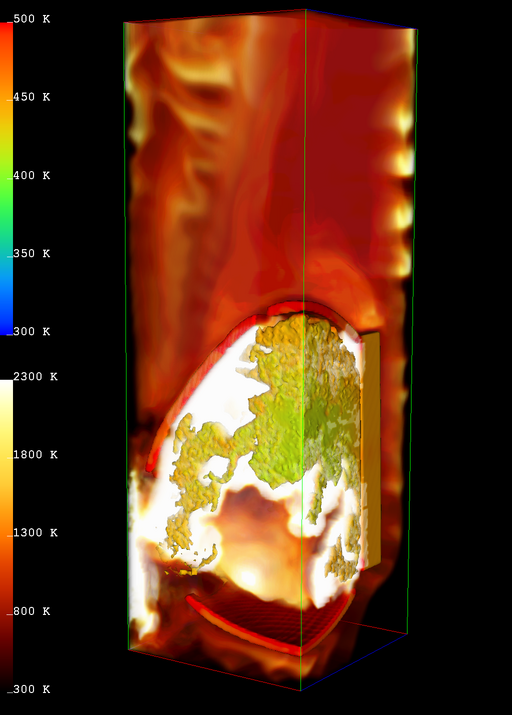
\includegraphics[scale=0.5]{fire-container-explosion-scirun.png}
  \caption{Target Simulation - Fire-Container-Explosion.}
  \label{Fig:fire-container-explosion}
\end{wrapfigure}
%\end{figure}


Complex simulations such as this require both immense computational
power and complex software. Typical simulations include solvers for
structural mechanics, fluids, chemical reactions, and material
models. All of these aspects must be integrated in an efficient manner
to achieve the scalability required to perform these simulations. The
heart of Uintah is a sophisticated computational framework that can
integrate multiple simulation components, analyze the dependencies and
communication patterns between them, and efficiently execute the
resulting multi-physics simulation.  Uintah also provides mechanisms
for automating load-balancing, checkpoint/restart, and parallel
I/O. The Uintah core was designed to be general, and is appropriate
for use in a wide range of PDE algorithms based on structured
(adaptive) grids and particle-in-cell algorithms.


\section{Uintah Software}

The Uintah Computational Framework (also referred to as Uintah or the UCF)
consists of a set of software components and libraries that facilitate
the solution of Partial Differential Equations (PDEs) on Structured
AMR (SAMR) grids using up to hundreds to thousands of processors.

One of the challenges in designing a parallel, component-based and
multi-physics application is determining how to efficiently decompose
the problem domain. Components, by definition, make local
decisions. Yet parallel efficiency is only obtained through a globally
optimal domain decomposition and scheduling of computational
tasks. Typical techniques include allocating disjoint sets of
processing resources to each component, or defining a single domain
decomposition that is a compromise between the ideal load balance of
multiple components. However, neither of these techniques will achieve
maximum efficiency for complex multi-physics problems.

Uintah uses a non-traditional approach to achieving parallelism by
employing an abstract task graph representation to describe
computation and communication. The task graph is an explicit
representation of the computation and communication that occur in the
coarse of a single iteration of the simulation (typically a timestep
or nonlinear solver iteration). Uintah components delegate decisions
about parallelism to a scheduler component by using variable
dependencies to describe communication patterns and characterizing
computational workloads to facilitate a global resource
optimization. The task graph representation has a number of
advantages, including efficient fine-grained coupling of multi-physics
components, flexible load balancing mechanisms and a separation of
application concerns from parallelism concerns. However, it creates a
challenge for scalability which we overcome by creating an implicit
definition of this graph and representing it in a distributed fashion.

%\begin{figure}
%  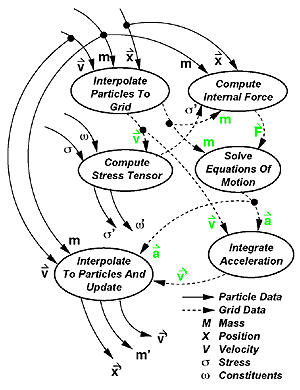
\includegraphics[scale=1]{Taskgraph-diagram.png}
%  \caption{Example Task Graph}
%  \label{fig:TaskGraph}
%\end{figure}

The primary advantage of a component-based approach is that it
facilitates the separate development of simulation algorithms, models,
and infrastructure. Components of the simulation can evolve
independently. The component-based architecture allows pieces of the
system to be implemented in a rudimentary form at first and then
evolve as the technologies mature. Most importantly, Uintah allows the
aspects of parallelism (schedulers, load-balancers, parallel
input/output, and so forth) to evolve independently of the simulation
components. Furthermore, components enable replacement of computation
pieces without complex decision logic in the code itself.

Please see the Developers Guide
(\url{http://www.uintah.utah.edu/trac/chrome/site/UintahAPI.pdf}) for more
information about the internal architecture of Uintah.

\subsection{Software Ports}

Uintah has been ported and runs well on a number of operating
systems.  These include Linux, Mac OSX, Windows, AIX, and HPuX. Simulating
small problems is perfectly feasible on 2-4 processor desktops, while
larger problems will need 100s to 1000s of processors on large
computer clusters. 

\subsection{Uintah Software History}

The UCF was orginally build upon the SCIRun Problem Solving
Environment.  SCIRun provided a core set of software building blocks,
as well as a powerful visualization package.  While Uintah continues
to use the SCIRun core libraries, Uintah's use of the SCIRun PSE has
been retired in favor of using the VisIt visualization package from
LLNL.


\section{Computational Framework} \label{Sec:UCF}

%__________________________________
\subsection{Time related variables}
\begin{Verbatim}[fontsize=\footnotesize]
   <Time>
       <maxTime>            1.0        </maxTime>
       <initTime>           0.0         </initTime>
       <delt_min>           0.0         </delt_min>
       <delt_max>           1.0         </delt_max>
       <delt_init>          1.0e-9      </delt_init>
       <max_delt_increase>  2.0        </max_delt_increase>
       <timestep_multiplier>1.0         </timestep_multiplier>
       <max_Timestep>       100        </max_Timestep>
   </Time>
\end{Verbatim}
%
%__________________________________
\subsection{Data Archiver}
- variable labels\\
- checkpointing \\
- different options for specifying the output frequency\\
%
%__________________________________
\subsection{Geometry objects}
- different objects available and how to specify them\\
- what is res \\
- operators, union, difference\\
%
%__________________________________
\subsection{Grid specification}
Explain how a grid is specified and what these tags mean

\begin{Verbatim}[fontsize=\footnotesize]
       <Level>
           <Box label="1">
              <lower>        [0,0,0]          </lower>
              <upper>        [5,5,5]          </upper>
              <extraCells>   [1,1,1]          </extraCells>
              <patches>      [1,1,1]          </patches>
           </Box>
           <spacing>         [0.5,0.5,0.5]    </spacing>
       </Level>
 \end{Verbatim}
%
%__________________________________
\subsection{Adapative Mesh Refinement}
- need to discuss the input options for the different regridders.
- How is a cell flagged as needing to be refined
%
%__________________________________
\subsection{load Balancer}
- to be filled in

%______________________________________________________________________
%   Notes to authors
% Please disable your editor's auto newline wrapping feature.  
% Please format \itemize sections 
%______________________________________________________________________



\chapter{Uda Management } \label{Chapter:UDA}
Uintah offers a number of tools for managing Uintah Data Archives (``UDAs''). These tools are especially useful for large simulations with large output.  These tools are used for quickly moving data, reducing the size and number of variables within your UDA and combining multiple UDAs. 

\iffalse
%______________________________________________________________________
\section{ReduceUda}
The typical mode of operation with production runs is to save all the variables you think you'll ever want to analyze, run the series of simulations, look at the data and then sit on the udas until you're forced to move them or delete them.  To help manage the size of the udas there's a new component(reduce\_uda) that allows users to prune out variables from an existing udas.   This component takes your existing uda,reads the input.xml file, and outputs the modified set of variables to a new uda, leaving the original uda untouched.
Below are instructions:
\begin{enumerate}
\item In the input.xml file set the simulation component type to ``reduce\_uda'', 

$<$SimulationComponent type=``reduce\_uda''/$>$
\item To avoid confusion with the original directory  change the uda name
   $<$filebase$>$UDA-diet.uda$<$/filebase$>$

\item Modify the DataArchiver section to restrict the data that will be saved.  Below are the available options:
   \begin{itemize}
     \item Resave the variables as floats using $<$outputDoubleAsFloat/$>$
     \item Remove variables from an uda by commenting them out
     \item For each variable limit the materials that are saved by using the 
    
     ``material=X'' option in the save label spec.
     \item For each variable limit the levels that it is saved on by using ``levels=X'' option in the save labels spec.
  \end{itemize}
For example to convert all of the doubles variables to floats and limit the variable vel\_CC to be
saved for material 1 make the following changes:

$<$outputDoubleAsFloat/$>$

$<$save label=``vel\_CC'' material=``1''/$>$


\item run the following command.

    mpirun -np X sus -reduce\_uda $<$name of uda directory$>$
    
    This will produce a new uda directory with the pruned variables. All time steps and checkpoints will be copied along with the index.xml, input file, input.xml and .dat files.

\end{enumerate}

When using this tool please be aware of the following:
\begin{itemize}
   \item If you're using this on a machine with a reduced set of system calls (tukey) configure with
          (- -with-boost)  This will enable the boost copy functions.
    \item Reduce\_uda will not work on ALCF machines (expect tukey)
    \item You must manually copy all On-the-Fly files/directories from the original uda
to the new uda, reduce\_uda ignores them.
    \item The $<$outputInterval$>$, $<$outputTimestepInterval$>$ tags are ignored and every
      timestep in the original uda is processed.  If you want to prune timesteps
      you must manually delete timesteps directories and modify the index.xml file.
    \item Use a different uda name for the modifed uda to prevent confusion with the original uda.
    \item In the timestep.xml files the following non-essential entries will be changed:
    
           numProcs:      Number of procs used during the reduceUda run.
           
           oldDelt:       Difference in timesteps, i.e., time(TS) - time (TS-1), in physical time.
           
           proc:          The processor to patch assignment.
    \item The number of files inside of a timestep directory will now equal the number of processors used to reduce the uda.
        You should use the same number of processors to reduce the uda as you will use to visualize it.
         For large runs this should speed up data transfers and post processing utilities.

    \item Checkpoint directories are copied with system calls from the original -$>$ modified uda.
      Only 1 processor is used during the copy so this will be slow for large checkpoints directories.
      Consider moving this manually.
    \item ALWAYS, ALWAYS, ALWAYS verify that the new (modified) uda is consistent
      with your specfications before deleting the original uda.
 \end{itemize}
\fi
%______________________________________________________________________
\section{pscp2}
pscp2 is a tool to quickly transfer data in parallel between two machines. In order for this to work there must be an password-less connection between the two machines. pscp2 is located in /src/scripts/udaTransferScripts/
\\
The usage is 
\begin{Verbatim}[fontsize=\footnotesize]
 ./pscp2 <# processors> 
         <transfer entire uda (y/n)> 
         <remove remote directory (y/n)> 
         < name of local directory> 
         <login@remote machine>:<remote path>
\end{Verbatim}

The following example shows the usage of pscp2 for transferring 1.uda.000 from the local machine to the home directory on ember using 8 processors. It will remove any files in the home directory on ember with the same title of 1.uda.000 but the original copy on the local machine will not be removed.

\begin{Verbatim}
 ./pscp2 8 y n 1.uda.000 username@ember.chpc.utah.edu:/home/
\end{Verbatim}

%______________________________________________________________________
\section{Make Master Uda}
makeMasterUda\_index.csh is a script used to combine multiple udas. This is useful when a simulation must be restarted multiple times and post processing is required. Instead of having to do post processing on each individual uda, makeMasterUda\_index.csh will combine all of the udas to allow for continuous analysis of the simulation start to finish.  The script is located at: src/scripts/makeMasterUda\_index.csh and it depends on the helper script: src/scripts/makeCombinedIndex.sh. The original udas must not be moved or the  masterUda will not find the udas. No changes will be made to the original udas.
\\
The usage is 
\begin{enumerate}
\item mkdir $<$masterUda$>$ This is where all of the udas will be linked together
\item cd $<$masterUda$>$
\item makeMasterUda\_index.csh ../uda.000 ../uda.001 ../uda.00N
\end{enumerate}

%______________________________________________________________________
\section{pTarUda}
pTarUda is a tool used to create/extract compressed tar files of each timestep in a UDA, including the checkpoints directory. pTarUda was designed to run in parallel and works well on udas with a large number of files and/or uncompressed data.  What it will buy you is faster moves, copies and transfers since the OS doesn't have to process as many files.  For uncompressed UDAs you may see up to a 30\% reduction in size. The original timestep directories are not deleted unless the -deleteOrgTimesteps option is used. This tool is found in /src/scripts/udaTransferScripts.
\\
Usage:
\begin{Verbatim}[fontsize=\footnotesize]
pTarUda -<create/extract> -uda <UDA directory name>

  Options:
  -np <int>:                 Number of processors. Default is 10                           
  -allTimesteps <y/n>:       Operate on all directories in uda? Default is yes.            
                             If "n" then a vi window will open allowing you                
                             to edit a list of timesteps to archive/extract.               
  -deleteOrgTimesteps        Delete original timestep directories after they have          
                             been tarred/untarred.                                         
  -continueTarring:          Continue tarring/untarring if previous attempts failed        
  -help:                     Display options summary                                       
\end{Verbatim}
\normalsize




\chapter{Arches}

\section{Introduction}
%
The ARCHES component was initially designed for predicting the heat-flux from large buoyant pool fires with potential hazard hazards immersed in or near a pool fire of transportation fuel.  Since then, this component has been extended to solve many industrially relevant problems such as industrial flares, oxy-coal combustion processes, and fuel gasification.  

The ARCHES component solves the conservative, finite volume, compressible, low-mach formulation of the Navier-Stokes equation with a pressure projection that includes the effect of variable density, reaction, and heat transfer modes in the gas phase including radiation.  Given the wide range of length and time scales that are present in many combustion problems of interest, ARCHES utilizes models for bridging the molecular (micro) scales to the full, large (macro) scales.  This bridging occurs through the use of subgrid and resolved scale mixing, reaction, and turbulence models. For example, momentum turbulence closure is accomplished by using various large eddy simulation (LES) type closure models. Fast chemistry scales are modeled by preprocessing the full chemical mechanism, modeled in various idealized configurations (e.g., equilibrium or flamelets), then tracking a set of reduced parameters on the LES mesh that map the full thermochemical state-space.  In general, the chemistry is tabulated and stored in a reaction table.  Subgrid turbulence species mixing processes and included by using presumed PDF methods and using models for certain moments of the distribution (e.g., scalar variance and mixture fraction).  The turbulence-species subgrid interaction model description are termed mixing models.  The chemistry and mixing models are usually completely preprocessed together into one tabular format to give a mixing table.  

Note that the sister component, MPMARCHES, couples an MPM description of a solid object to include stationary solids with and without conjugate heat transfer. While run as a separate component, MPMARCHES is simply a wrapped version of ARCHES to include the MPM interface.  

The following gives a brief introduction to a few of the key concepts of the Arches formulation of the transport equations and physical models as well as the CFD algorithm.  Following this explanation, an overview of the ARCHES input parameters are given.  

\section{Governing Equations}
%
The essential governing equations for the Arches component, written
in finite volume form, include the mass balance, momentum balance,
mixture fraction balance, and energy balance equations. Using a bold-face
symbol to represent a vector quantity, the equations are: 
\begin{enumerate}
\item The mass balance, \begin{equation}
\int_{V}\frac{\partial\rho}{\partial t}dV+\oint_{S}\rho\mathbf{u}\cdot d\mathbf{S}=0\;,\label{eqn:mass_balance}\end{equation}
 where $\rho$ is density and $\mathbf{u}$ is the velocity vector. 
\item The momentum balance, \begin{equation}
\int_{V}\frac{\partial\rho\mathbf{u}}{\partial t}dV+\oint_{S}\rho\mathbf{uu}\cdot d\mathbf{S}=\oint_{S}\tau\cdot d\mathbf{S}-\int_{V}\nabla pdV+\int_{V}\rho\mathbf{g}dV\;,\label{eqn:mom_balance}\end{equation}
 where $\tau$ is the deviatoric stress tensor defined as $\tau_{ij}=2\mu S_{ij}-\frac{2}{3}\mu\frac{\partial u_{k}}{\partial x_{k}}\delta_{ij}$,
the second isotropic term in $\tau_{ij}$ is absorbed into the pressure
projection for the current low-Mach scheme, and $S_{ij}=\frac{1}{2}\left(\frac{\partial u_{i}}{\partial x_{j}}+\frac{\partial u_{j}}{\partial x_{i}}\right)$.
Also in Equation \ref{eqn:mom_balance}, $\mathbf{g}$ is the gravitational
body force and $p$ is pressure. 
\item The mixture fraction balance, \begin{equation}
\int_{V}\frac{\partial\rho f}{\partial t}dV+\oint_{S}\rho\mathbf{u}f\cdot d\mathbf{S}=\oint_{S}D\nabla f\cdot d\mathbf{S}\;,\label{eqn:species_balance}\end{equation}
 where $f$ is the mixture fraction and a Fick's law form of the diffusion
term assuming equal diffusivities results in a single diffusion coefficient,
$D$. 
\item The thermal energy balance, \begin{equation}
\int_{V}\frac{\partial\rho h}{\partial t}dV+\oint_{S}\rho\mathbf{u}h\cdot d\mathbf{S}=\oint_{S}k\nabla h\cdot d\mathbf{S}-\oint_{S}q\cdot d\mathbf{S}\;,\label{eqn:heat_balance}\end{equation}
 where $h$ is the sum of the chemical plus sensible enthalpy, $q$
is the radiative flux, a Fourier's law form of the conduction term
is used with a diffusion coefficient, $k$, and the pressure term
is neglected. 
\end{enumerate}
These equations are solved in an LES context, meaning filters are
applied to the equations. Here, we use Favre filtering, defined as
\[
\overline{\phi}=\frac{\overline{\rho\phi}}{\overline{\rho}},\]
 to isolate the density in the filtered equations. The filtering operations
result in the classic turbulence closure problem and thus models are
required. 

Consider a control volume, $V$, with surface area $S$.  Because the equations will be  solved on a computational grid, one can safely assume that the the control volume has $N$ faces, where unique faces are identified with their index, $k$.  The discussion is further simplified by only considering cubic volumes with length $h$.  
Given the cubic control volume, a surface-filtered field for a variable $\phi$ is defined as $\overline{\phi}^{(j)}(\mathbf{x})$, where the variable is filtered on a plane in the $x_j$ orthogonal direction.  Then, for any surface, $k$, the field is sampled at the face centered location.  For example, if $j=1$, the surface-filtered quantity is
%
\begin{equation}
\overline{\phi}^{2d, (1)}(\mathbf x) = \frac{1}{h^2} \int_{x_2 - h/2}^{x_2 + h/2}  \int_{x_3 - h/2}^{x_3 + h/2} \phi(\mathbf x') dx_2' dx_3' \; .
\end{equation} 
%
The volume average follows as
%
\begin{equation}
\overline{\phi}^{3d} (\mathbf x) = \frac{1}{h^3} \int_{x_1 - h/2}^{x_1 + h/2} \int_{x_2 - h/2}^{x_2 + h/2}  \int_{x_3 - h/2}^{x_3 + h/2} \phi(\mathbf x') dx_1' dx_2' dx_3' \; .
\end{equation}
%
The bars over the variable, $\phi$, are labeled with `2d' and `3d' superscripts to distinguish between the two filters.  Pope \cite{Pope179} identifies the proceeding definitions as using the ``anisotropic box" filter kernel where the resultant variables are simply averages over the intervals $x_j - \frac{1}{2}h < x_j' < x_j + \frac{1}{2}h$. 

For convenience in isolating density in the filtered equations, a Favre-filtered quantity is defined for an arbitrary variable, $\varphi$, as 
%
\begin{equation}\label{eqn:favre_surf}
\widetilde{\varphi}^{2d} \equiv \frac{\overline{\rho \varphi}^{2d}}{\overline{\rho}^{2d}} \; ,
\end{equation}
%
and
%
\begin{equation}\label{eqn:favre_vol}
\widetilde{\varphi}^{3d} \equiv \frac{\overline{\rho \varphi}^{3d}}{\overline{\rho}^{3d}} \;.
\end{equation}
%
Because the 2d and 3d filters are explicitly defined, this convention is slightly different than what is normally observed in the literature.  Most literature, however, derives the filtered equations from the finite difference equations rather than the finite volume equations.  Thus, using $\overline{\rho}^{2d}$ and $\overline{\rho}^{3d}$ in Equations \ref{eqn:favre_surf} and \ref{eqn:favre_vol} to stress surface and volume filtered densities are appropriate for the present discussion.

The previous definitions are applied to the integral forms of the governing equations to obtain the Favre-filtered LES equations.  Nevertheless, there are terms in the Favre-filtered equations that cannot be solved.  These include the surface filtered convection of momentum, $\widetilde{u_i u}^{2d}_j$, the surface filtered convection of mixture fraction, $\widetilde{u_j f}^{2d}$, and the surface filtered convection of enthalpy, $\widetilde{u_j h}^{2d}$.  

For the filtered velocity product, $\overline{\rho}^{2d} \; \widetilde{ u_i u}^{2d}_j$, a subgrid stress tensor is defined as, 
%
\begin{equation}\label{eqn:tau_sgs}
\tau^{sgs}_{ij} = \widetilde{u_i u}^{2d}_j - \widetilde{u}^{2d}_i \widetilde{u}^{2d}_j \; .
\end{equation}
%
Similarly, subgrid diffusion terms are defined for mixture fraction and enthalpy, 
%
\begin{eqnarray}
\mathcal{J}^{f}  = \widetilde{u_j f}^{2d} - \widetilde{u}^{2d}_j \widetilde{f}^{2d} \;, \\
\mathcal{J}^{h} = \widetilde{u_j h}^{2d} - \widetilde{u}^{2d}_j \widetilde{h}^{2d} \; .\\
\end{eqnarray}

Using these definitions, the final form of the Favre-filtered equations is
%
\begin{enumerate}
\item The filtered mass balance, 
%
\begin{equation}\label{eqn:filtered_mass_balance}
\frac{d}{d t} \left(\widetilde{\rho}^{3d} \right)   + \frac{S_k}{V} n_{kj} \left( \overline{\rho}^{2d} \; \widetilde{u}^{2d}_j \right) = 0 \; .
\end{equation}
%
\item The filtered momentum balance, 
%
\begin{equation}\label{eqn:filtered_mom_balance}
\frac{d}{d t} \left( \overline{\rho}^{3d} \; \widetilde{u}^{3d}_i \right) = \frac{S_{k}}{V} n_{kj}\left( -\overline{\rho}^{2d} \; \widetilde{u}^{2d}_i\widetilde{u}^{2d}_j + \overline{\tau}^{2d}_{ij} + \tau^{sgs}_{ij} - \overline{p}^{2d} \delta_{ij} \right) + \overline{\rho}^{3d} \; g_i  \; .
\end{equation}
%
\item The filtered mixture fraction balance,
%
\begin{equation}\label{eqn:filtered_mixfrac_balance}
\frac{d}{d t} \left( \overline{\rho}^{3d} \; \widetilde{f}^{3d} \right) = \frac{S_k}{V} n_{kj} \left( -\overline{\rho}^{2d} \; \widetilde{u}^{2d}_j \widetilde{f}^{2d} + D \nabla \overline{f}^{2d} + \mathcal{J}^{f} \right) \; .
\end{equation}
%
%
\item The filtered thermal energy balance, 
%
\begin{equation}\label{eqn:filtered_heat_balance}
\frac{d}{d t} \left( \overline{\rho}^{3d} \; \widetilde{h}^{3d} \right) = \frac{S_{k}}{V} n_{kj} \left( -\overline{\rho}^{2d} \; \widetilde{u_j}^{2d}\widetilde{h}^{2d} + k \nabla \overline{h}^{2d}  - \overline{q}^{2d}  + \mathcal{J}^h \right) \; .
\end{equation}
%
\end{enumerate}
The subgrid momentum stress, $\tau_{ij}^{sgs}$, the subgrid mixture fraction dissipation, $\mathcal{J}^{f}$, and the subgrid heat dissipation, $\mathcal{J}^{h}$, contain the unresolved or subgrid action of the turbulence on the transported quantities.  Since these terms arise from definitions, models are introduced to include the subgrid effects that they represent.  These models are discussed next.

\subsection{Subgrid Turbulence Models}
%
The construction of both $\mathcal{J}^f$ and $\mathcal{J}^{h}$ is relatively straight forward. Invoking an ``eddy-viscosity" modeling concept, the subgrid transport due to turbulent advection is treated as an enhanced diffusion term for the unclosed terms listed above.   That is, the subgrid mixture fraction dissipation and subgrid enthalpy dissipation are respectively written as, 
%
\begin{equation}
\mathcal{J}^{f} = D_{t} \frac{\partial \overline{f}^{2d}}{\partial x_j} \; , 
\end{equation}
%
and 
%
\begin{equation}
\mathcal{J}^{h} = k_{t} \frac{\partial \overline{h}^{2d}}{\partial x_j} \; .
\end{equation}
%
To model $D_{t}$ and $k_{t}$, constant turbulent Schmidt ($Sc_t$),
%
\begin{equation}\label{eqn:subgrid_mixfrac}
Sc_{t} = \frac{1}{\rho} \frac{\mu_t}{D_t} \; ,
\end{equation}
%
and Prandlt ($Pr_t$), 
%
\begin{equation}\label{eqn:subgrid_enthalpy}
Pr_{t} = \frac{1}{\rho} \frac{\mu_t}{k_t} \; ,
\end{equation}
%
numbers are assumed with where $\mu_t$ is a turbulent viscosity.  Following Pitsch and Steiner \cite{pitsch2000}, the values of the turbulent Schmidt and Prandlt number are taken as $Sc_t = Pr_t = 0.4$, which is consistent with a unity Lewis number assumption.  

For the subgrid scale stress tensor, $\tau^{sgs}_{ij}$, two common LES turbulence closure models are the constant coefficient Smagorinsky model \cite{Smagorinsky178} and the dynamic coefficient Smagorinsky model \cite{Moin158}.  As with the scalar subgrid modeling terms, the eddy viscosity model is again invoked for $\tau^{sgs}_{ij}$.  Defining the deviatoric subgrid stress tensor as, 
%
\begin{equation}
\tau^{d, sgs}_{ij} = \tau^{sgs}_{ij} - \frac{1}{3}\tau^{sgs}_{kk} \delta_{ij}, 
\end{equation}
%
the subgrid stress is taken as,
%
\begin{equation}
\tau_{ij}^{d, sgs} \approx -2 \nu_t \overline{S}_{ij} = -2 (C_s \Delta)^2 |\overline{S}|\overline{S}_{ij} \; , 
\end{equation}
%
where $\Delta$ is the filter width, $\nu_t$ is the eddy viscosity and $|\overline{S}| \equiv (2\overline{S}_{ij}\overline{S}_{ij})^{1/2}$.  For the Smagorinsky model,  $C_s \approx 2$  depending on the filter type, numerical method, and flow configuration \cite{Pope179}.  

For the dynamic Smagorinsky model, $C_s$ is computed by taking a least squares approach to determining the length scale \cite{Lilly180},
%
\begin{equation} \label{eqn:cs_eqn}
(C_s \Delta)^2 = \frac{ \left< \mathcal{L}_{ij} M_{ij} \right>}{ \left< M_{ij}M_{ij} \right> } \; ,
\end{equation}
%
where
%
%
\begin{equation}
\mathcal{L}_{ij} = 2( C_s \Delta)^2 \widehat{ |\overline{S} | \overline{S} }_{ij} - 
   2( C_s \widehat{\Delta})^2 \widehat{ |\overline{S}} | \widehat{\overline{S}}_{ij} \; ,
\end{equation}
%   
and
\begin{equation}
M_{ij} \equiv 2 \left( \widehat{ | \overline{S} | \overline{S} }_{ij} - \alpha^2 |\widehat{\overline{S}}|\widehat{\overline{S}}_{ij} \right) \; .
\end{equation} 
%
The hat defines an explicit test filter and the angled brackets in Equation \ref{eqn:cs_eqn} conceptually represent an averaging over a homogeneous region of space that, experience has shown, is necessary for stability.  Experience has also shown that averaging over the test filter width is adequate and the filter width ratio, $\alpha = \widehat{\Delta}/\Delta$, is usually taken to be 2.

\subsection{Subgrid Momentum Dissipation}
%%
Addressing the momentum closure involves finding a suitable model for the subgrid scale stress tensor, $\tau^{sgs}_{ij}$.  Two common LES turbulence closure models are examined: the constant coefficient Smagorinsky model and the dynamic coefficient Smagorinsky model.  
%%
In LES modeling, field variables are decomposed into a spatially filtered field and a residual component, $u = \overline{u} + u'$.  This decomposition is known as a Leonard decomposition.  While seemingly similar to a Reynolds decomposition used in Reynolds Averaged Navier-Stokes (RANS) models, the Leonard decomposition has the property that the filtered residual component is generally not equal to zero, $\overline{u'} \neq 0$.  As a result, the subgrid stress term contains several terms, 
%%%
\begin{eqnarray}
\tau_{ij}^{sgs} = \overline{ \left(\overline{u}_i + u_i' \right) \left(\overline{u}_i + u_i' \right)} - \overline{u}_i \overline{u}_j \; , \; \; \; \; \; \; \; \; \; \; \; \; \; \;  \; \; \nonumber \\
= \underbrace{\overline{\overline{u}_i \overline{u}_j} - \overline{u}_i \overline{u}_j}_{L_{ij}}  + 
   \underbrace{\overline{\overline{u}_i {u}_j'} + \overline{{u}_i' \overline{u}_j}}_{C_{ij}} + 
   \underbrace{ \overline{u_i' + u_j'} }_{R_{ij}} \; , 
\end{eqnarray}
%
referred to as the Leonard stress, the cross stresses, and the Reynolds stress respectively.  

It is useful to consider the physical interpretation of the various components of the stress. The Leonard term is responsible for filtering and projecting the nonlinear interactions of the resolved components back to the finite LES space.  This is a correction to the resolved advective term in accordance with the stated explicit filter used to derive the LES equations. It does not account for aliasing errors. The first cross term represents advection of the resolved field by turbulent fluctuations. The second cross term represents the advection of subgrid scales by the resolved field. The Reynolds stress is familiar from RANS and represents the advection of subgrid scales by turbulent fluctuations. 

As with the scalar subgrid modeling terms, the eddy viscosity model is again invoked for $\tau^{sgs}_{ij}$.  The most common eddy viscosity model in LES is the Smagorinsky model \cite{Smagorinsky178}.  Defining the deviatoric subgrid stress tensor as, 
%%
\begin{equation}
\tau^{d, sgs}_{ij} = \tau^{sgs}_{ij} - \frac{1}{3}\tau^{sgs}_{kk} \delta_{ij}, 
\end{equation}
%%
the subgrid stress is approximated by,
%%
\begin{equation}
\tau_{ij}^{d, sgs} \approx -2 \nu_t \overline{S}_{ij} = -2 (C_s \Delta)^2 |\overline{S}|\overline{S}_{ij} \; , 
\end{equation}
%%
where, $\Delta$ is the filter width, $\nu_t$ is the eddy viscosity, $|\overline{S}| \equiv (2\overline{S}_{ij}\overline{S}_{ij})^{1/2}$, and typically $C_s \approx 2$  depending on the filter type, numerical method, and flow configuration \cite{Pope179}. This model is basically identical to Prandtl's mixing length model with $l = C_s \Delta$.

The dynamic procedure \cite{Germano74, Moin158} eliminates the need to specify the model constant, $C_s$, a priori, with the basic assumption that the constant is the same for two different filter scales. The smaller scale is historically referred to as the ``grid scale" (though the filter width need not equal the grid spacing, $\Delta \geq h$)), and the larger scale is referred to as the ``test scale".  Implicit in this assumption is the requirement that both scales lie within the inertial subrange. 

Defining the deviatoric residual stress tensor as, 
\begin{equation}
T_{ij}^d = T_{ij} - \frac{1}{3} T_{kk}\delta_{ij} \;,
\end{equation}
the residual stress at the test scale is given by,
%%
\begin{equation}\label{eqn:res_stress}
T_{ij}^{d} \equiv \overline{\widehat {u_i u_j}} - \overline{\widehat{u}}_i \overline{\widehat{u}}_j \approx -2(C_s \widehat{\Delta})^2 |\widehat{\overline{S}}| \widehat{\overline{S}}_{ij} \; .
\end{equation}
%%
where $\widehat{\Delta}$ is the test filter width and the hat defines an explicit test filter. By test filtering Equation \ref{eqn:tau_sgs} and combining this with \ref{eqn:res_stress}, one can construct the Leonard term, $\mathcal{L}_{ij}$. This is also known as the ``Germano identity",
%%
\begin{equation}
\mathcal{L}_{ij} = T_{ij} - \widehat{ \tau^{sgs}}_{ij} =  \overline{\widehat {u_i u_j}} - \overline{\widehat{u}}_i \overline{\widehat{u}}_j \; .
\end{equation}
%%
Notice that the Leonard term is directly computable from resolved LES quantities. By restating the Smagorinsky model in terms of the Germano identity, one ends up with an over-determined system of equations for the unknown, $C_s$,
%%
\begin{equation}
\mathcal{L}_{ij} = 2( C_s \Delta)^2 \widehat{ |\overline{S} | \overline{S} }_{ij} - 
   2( C_s \widehat{\Delta})^2 \widehat{ |\overline{S}} | \widehat{\overline{S}}_{ij} \; .
\end{equation}
%%   
Although we have pulled $C_s$ out of the test filtering operation of the subgrid stress, this approximation yields acceptable results. In practice, one takes a least squares approach to determining the length scale \cite{Lilly180},
%%
\begin{equation} \label{eqn:cs_eqn}
(C_s \Delta)^2 = \frac{ \left< \mathcal{L}_{ij} M_{ij} \right>}{ \left< M_{ij}M_{ij} \right> } \; ,
\end{equation}
%%
where
%%
\begin{equation}
M_{ij} \equiv 2 \left( \widehat{ | \overline{S} | \overline{S} }_{ij} - \alpha^2 |\widehat{\overline{S}}|\widehat{\overline{S}}_{ij} \right) \; .
\end{equation} 
%%
The only model parameter, then, is the filter width ratio, $\alpha = \widehat{\Delta}/\Delta$, usually taken to be 2.

The angled brackets in Equation \ref{eqn:cs_eqn} conceptually represent averaging over a homogeneous region of space which, experience has shown, is necessary for stability. We have found that averaging over the test filter width is adequate.
%%
With these implementation practices, the dynamic model is generally robust. The implementation can be made more efficient by computing the constant roughly every 10 time steps (based on the advective CFL), and only for the first Runge-Kutta step.

\subsection{LES Algorithm}\label{Sec:LES_Algorithm}
%
The set of filtered equations (Equations \ref{eqn:filtered_mass_balance}-\ref{eqn:filtered_heat_balance}) are discretized in space and time and solved on a staggered, finite volume mesh.  The staggering scheme consists of four offset grids. One grid stores the scalar quantities and the remaining three grids store each component of the velocity vector. The velocity components are situated so that the center of their control volume is located on the face centers of the scalar grid in their respective direction.  Figure \ref{fig:staggered_grid} shows an example of a two-dimensional grid and the staggering arrangement.
%
%% Staggered Grid
\begin{figure}
 \begin{center}
    \scalebox{.85}{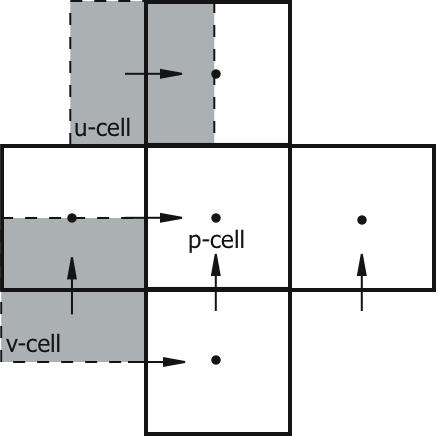
\includegraphics{staggered_grid.png}}
   \caption{Staggered grid arrangement in two dimensions with u and v velocity cell centers located on the face centers of the scalar cells.}\label{fig:staggered_grid}
   \end{center}
\end{figure}
%

The staggering arrangement is advantageous for computing low-Mach LES reacting flows.  First, since a pressure projection algorithm is used, the velocities are exactly projected without interpolation error because the location of the pressure gradient coincides directly with the location of the velocity storage location. Second, Morinishi et al. \cite{morinishi98} showed that kinetic energy is exactly conserved when using a central differencing scheme on the convection and diffusion terms without a subgrid model and in combination with a staggered grid.  Having a spatial scheme that conserves kinetic energy is advantageous because it limits artificial dissipation that arises from the differencing scheme.  These conservation properties make the staggered grid a prime choice for LES reacting flow simulation.

For the spatial discretization of the LES scalar equations, flux limiting and upwind schemes for the convection operator are used.  These schemes are advantageous for ensuring that scalar values remain bounded.  For the momentum equation, a central differencing scheme for the convection operator is used.  All diffusion terms are computed with a second order approximation of the gradient.  

When computing the 2d surface filtered field on the faces of the control volume, one is forced to use an interpolation from the 3d volume filtered field.  This approximation is tolerated because computing the 2d surface field is simply not possible with the given grid scheme. % This is a good example of how LES modeling issues and discrete numerics issue intertwine in applied LES modeling.     

%Jennifer edited
An explicit time stepping scheme is chosen.  A general, multistep explicit update for a variable, $\phi$, may be written as, 
%
%===== Explicit Update =====
\begin{eqnarray}\label{eqn:forward_euler}
\phi^0 = \phi^n \; , \nonumber \\
  \phi^{(i)} = V \sum_{k=0}^{m-1}
\left( \alpha_{i,k}  \phi^{(k)} +
\Delta t \beta_{i,k} L( \phi^{(k)}) \right) \; , \; \; \; \; i = 1, ..., m \\
\phi^{(m)} = \phi^{n+1} \; , \nonumber
\end{eqnarray}
%
where $n$ is the time level, $m$ is the substep between $n$ and $n+1$, $\alpha$ and $\beta$ are integration coefficients, and $L$ is a linearization operator on the the convective flux and source terms.
%
Letting $m=1$ and $\alpha = \beta = 1$ the forward-Euler time
integration scheme is determined,
%%
%%===== Forward Euler =====
\begin{equation}\label{eqn:forward_euler}
\left(  \phi \right)^{n+1} = \left(
\phi \right)^{n} + \Delta t (L( \phi)^n) \; .
\end{equation}
%%
A higher order, multistep method is derived by letting $m > 1$ and
choosing appropriate constants for $\alpha$ and $\beta$. For this
study, two step and three step, strong stability preserving (SSP)
coefficients were chosen from Gottlieb et al.
\cite{Gottlieb75}.

Using the coefficients given by Gottlieb et al., the SSP-RK 2 stepping scheme is
%%
%%===== second order time stepping =====
\begin{eqnarray}\label{eqn:rk_second_order}
( \phi)^{(1)} = ( \phi)^{n} + \Delta
t (L(\phi)^n) \\ \nonumber
( \phi)^{n+1} = \frac{1}{2}(
\phi)^{n} + \frac{1}{2}( \phi)^{1} +
\frac{1}{2}\Delta t (L( \phi)^{(1)}) \;.
\end{eqnarray}
%%
SSP-RK 3 time stepping scheme is,
%%
%%===== third order time stepping =====
\begin{eqnarray}\label{eqn:rk_second_order}
(\phi)^{(1)} = (\phi)^{n} + \Delta t (L(\phi)^n) \\ \nonumber
(\phi)^{(2)} = \frac{3}{4}(\phi)^{n} + \frac{1}{4}( \phi)^{(1)} +
\frac{1}{4}\Delta t (L( \phi)^{(1)}) \\ \nonumber ( \phi)^{(n+1)} =
\frac{1}{3}(\phi)^{n} + \frac{2}{3}(
\phi)^{(2)} + \frac{1}{4}\Delta t (L(
\phi)^{(2)}) \; .
\end{eqnarray}
%%

The time step is limited by
%
\begin{equation}
\Delta t \leq c \Delta t_{F.E.}
\end{equation}
%
where $\Delta t_{F.E.}$ is the forward-Euler time step limited by
the Courant-Friedrichs-Levy condition and $c$ is a constant less
than or equal to one.  

A higher order, multistep method is derived by letting $m > 1$ and choosing appropriate constants for $\alpha$ and $\beta$. For this study, two step and three step, strong stability preserving (SSP) coefficients were chosen from Gottlieb et al. \cite{Gottlieb75}.  The coefficients for SSP-RK 2 and SSP-RK 3 are optimal in the sense that the scheme is stable when $c=1$ if the forward-Euler time step is stable for hyperbolic problems.  In practice, for the Navier-Stokes equations, the value of $c$ is taken less than one.

Choosing an explicit time stepping scheme, rather than an implict one, creates a challenge for solving the set of equations.  The density at the $n+1$ timestep, which is required to determine the cardinal variables,  requires an estimation.  Taking the estimated density for  $\overline{\rho}^{n+1}$ to be $\overline{\rho}^*$, the estimation can be as simple as $\overline{\rho}^* = \overline{\rho}^n$.  Note that the 2d and 3d filter distinction is dropped for the remainder of this discussion for the sake of simplicity.  A slightly more complicated procedure involves a forward-Euler step of the continuity equation to obtain $\overline{\rho}^*$.  This is written as,  
%
\begin{equation}\label{eqn:rho_update}
\overline{\rho}^{ *} = \overline{\rho}^{ n} - \Delta t \frac{S_k}{V} n_{kj} \left(  \overline{\rho} \widetilde{u_j} \right) \; .
\end{equation}
%

% FIXME: section reference is broken
Ideally, one would like to know $\overline{\rho}^{n+1}$ rather than an estimate.  While more details will be discussed in Section \ref{sec:combust_react_models}, one recognizes that $\rho$ is a function of the same variables that are being updated in time, namely, the mixture fraction, $f$, and enthalpy, $h$.  This quandary is a result of the explicit time stepping method will not be resolved for variable density flows without using a fully implicit method.  Explicit methods, however, do have advantages, especially for large scale parallel computations.  Specifically, explicit methods are easier to load balance because the amount of work required for each processor is readily determined a priori, which makes for an efficient parallel computation.  Explicit methods are also easier to code into a computer and to debug.  For these reasons, the current algorithm discussion is limited to explicit methods only. 

The explicit algorithm for solving the set of filtered equations is shown in Algorithm \ref{alg:LES_algorithm}.  
%
%\begin{lstlisting}[float, caption = Explicit LES algorithm, label=alg:LES_algorithm]
%for t:=t_{min} to t_{max} do 
%fill in later..
%for $RK_{step}$:=1 to $N$
%end;
%end; 
%\end{lstlisting}
%
\begin{algorithm}[t]
\caption{Explicit LES algorithm.}\label{alg:LES_algorithm}
%
\begin{algorithmic}[] %add [1] for #'s
\FOR{$t = t_{min}...t_{max}$}
\FOR{$RK_{step} = 1$...$N$} 
\STATE 	Solve for scalars products $(\overline{\rho} \widetilde{f})^{n+1}$ and $(\overline{\rho} \widetilde{h})^{n+1}$.
\STATE	Estimate $\overline{\rho}^* = \overline{\rho}^{n+1}$ from Equation \ref{eqn:rho_update}
\IF{$\overline{\rho}^* < \overline{\rho}_{min}$ or $ \overline{\rho}^* > \overline{\rho}_{max}$}
\STATE $\overline{\rho}^* = \overline{\rho}^{n}$
\ENDIF
\STATE Compute $\widetilde{f}^{n+1} = (\overline{\rho}\widetilde{f})^{n+1}/{\overline{\rho}^*}$ and $\widetilde{h}^{n+1} = (\overline{\rho}\widetilde{h})^{n+1}/{\overline{\rho}^*}$ 
\STATE Compute $\overline{\rho}^{n+1} = f(\widetilde{f}^{n+1}, \widetilde{h}^{n+1})$
\STATE Compute $\widetilde{\mathbf{u}}^*$, the unprojected velocities
\STATE Perform RK averaging if needed
\STATE Compute correct pressure from pressure poisson equation
\STATE Project velocities with correct pressure to get $\widetilde{\mathbf{u}}^{n+1}$ 
\ENDFOR
\ENDFOR
\end{algorithmic}
\end{algorithm}


\subsection{Direct Quadrature Method of Moments}\label{sec:DQMOM}

The direct quadrature method of moments (DQMOM) is a recently-developed moment method for tracking distributions.  It has been applied to distributions of evaporating droplets, soot particle distributions, fluidized beds, and subgrid chemistry PDFs. The method is similar to the quadrature method of moments (QMOM), in that it uses quadrature to provide closure for the moment transport equation; however, it differs in that the moment transport equations are not actually solved, unlike the quadrature method of moments (QMOM). Rather, the DQMOM tracks the quadrature weights and weighted abscissas representing the NDF directly, rather than using the product-difference algorithm to transform between a set of moments and quadrature weights and abscissas that would best represent that distribution.

The basic outline of the method, given below, defines and covers these fundamental steps and concepts:
\begin{enumerate}
\item Number Density Function (NDF)
\item Moments
\item Moment Methods for NDF Transport
\item Quadrature
\item Direct Quadrature Method of Moments
\end{enumerate}

The number density function is the starting point, as it is the function of interest that is being tracked.  Moments are defined, and moment methods are explained and applied to the NDF transport equation to yield the moment transport equation.  Furthermore, quadrature is defined and applied to approximate the moments, which leads to a quadrature-approximated moment transport equation.  This equation leads to the fundamental equations governing DQMOM.

\subsubsection{Number Density Function}\label{subsubsec:NDF}
Using the direct quadrature method of moments (DQMOM) in Arches, the dispersed phase is represented as a number density function (NDF), which is tracked in a stationary Eulerian reference frame. 
The NDF is denoted as $f$ and represents the number of particles at a particular point in space and time.  
Using DQMOM, this NDF is parameterized on several different variables - independent variables for the particles. 
These are called ``internal coordinates,'' and are denoted by $\boldsymbol{\xi}$ (where boldface denotes a vector quantity). 
In this case the NDF is written as $f\left(\boldsymbol{\xi};\boldsymbol{x},t\right)$.

The starting point for the DQMOM equations is the NDF transport equation; this is derived in several places and will not be derived here. The NDF transport equation is:
\begin{eqnarray}\label{eq:NDF transport equation}
  \dfrac{\partial f \left( \boldsymbol{\xi}; \boldsymbol{x},t \right)}{\partial t}  % accumulation term
  + \dfrac{\partial}{\partial x_{i}} \left( \left< u_{i} \vert \boldsymbol{\xi}; \boldsymbol{x}, t \right> f \left( \boldsymbol{\xi}; \boldsymbol{x},t \right) \right) & & \nonumber \\ % spatial convection term
  + \dfrac{\partial}{\partial \xi_{j}} \left( \left< G_{j} \vert \boldsymbol{\xi};\boldsymbol{x}, t \right> f \left( \boldsymbol{\xi}; \boldsymbol{x},t \right) \right)   % phase-space convection term
  & = & h \left( \boldsymbol{\xi}; \boldsymbol{x},t \right),
\end{eqnarray}

\noindent where $G_{j}$ is the velocity of the NDF in phase-space (that is, internal coordinate-space), and is defined by:
\begin{equation}
G_{j} = \dfrac{ d \xi_{j} }{d t}
\end{equation}

\noindent (note this is analogous to spatial velocity $v$, defined by:
\begin{equation}
v_{i} = \dfrac{ d x_{i} }{d t},
\end{equation}

\noindent and that $G_{j}$ takes the same form as Lagrangian particle models); also, $h$ is a birth and death term representing the appearance or disappearance of particles within the domain.  Note also that the velocities $v_i$ and $G_j$ are conditioned on the value of the internal coordinates, as well as on space and time. This implies that the spatial and phase-space velocities are full distributions in $\left( \boldsymbol{\xi}, \boldsymbol{x} \right)$ space, just as the NDF is.

The number of internal coordinates is denoted by $N_{\xi}$. If $N_{\xi} = 1$, the NDF is called ``univariate''; if $N_{\xi} > 1$, then the NDF is called ``multivariate''.



\subsubsection{Moments}\label{subsubsec:moments}
Using DQMOM, the particles are represented as an Eulerian distribution - that is, the particles are not treated in an individual sense, but in a statistical sense. In order to represent the NDF in the framework of a scalar CFD code, the NDF must be represented using a set of scalars that can be transported. One such set of scalars, the moments of the NDF, provide useful statistical information about the distribution. Additionally, a distribution can be approximately reconstructed from its moments. The first moment of the distribution represents the mean value; the second, the variance of the distribution; and so on. An arbitrary number of moments can be defined. For a univariate NDF, the $k^{th}$ moment of the NDF is defined as:
\begin{equation}\label{eq:univariate moment definition}
m_{k} = \dfrac{ \displaystyle{ \int_{-\infty}^{+\infty}{\xi^k f \left( \xi ; \boldsymbol{x},t \right) d\xi } } }{ \displaystyle{ \int_{-\infty}^{+\infty}{ f \left( \xi ; \boldsymbol{x},t \right) d\xi } } }
\end{equation}

Alternatively, if the NDF is a function of several internal coordinates, the $\boldsymbol{k}^{th}$ moment is defined as:
\begin{eqnarray}\label{eq:multivariate moment definition}
m_{\boldsymbol{k}} & = & \dfrac{ \displaystyle{ \dotsintop_{\infty}^{+\infty}{ \xi_{1}^{k_1} \dots \xi_{N_{\xi}}^{k_{N_{\xi}}}   f \left( \xi_1, \dots, \xi_{N_{\xi}} \right)   d\xi_1 \dots d\xi_{N_{\xi}} } }}
{  \displaystyle{ \dotsintop_{\infty}^{+\infty}{ f \left( \xi_1, \dots, \xi_{N_{\xi}} \right)   d\xi_1 \dots d\xi_{N_{\xi}} } } }
%m_{\boldsymbol{k}}  & = & \dfrac{ \displaystyle{ \dotsintop_{-\infty}^{+\infty} \xi_{1}^{k_1} \dots \xi_{N_{\xi}}^{k_{N_{\xi}}}   f \left( \xi_1, \dots \xi_{N_{\xi}} \right)   d\xi_1 \dots d\xi_{N_\xi} }{ \displaystyle{ } }
%				& = & 
\\
m_{\boldsymbol{k}} & = & \dfrac{{\displaystyle \dotsintop_{-\infty}^{+\infty}}\left[
\left({\displaystyle \prod_{m=1}^{N_{\xi}}}\xi_{m}^{k_{m}}\right)
\, f(\boldsymbol{\xi};\boldsymbol{x},t)\, d\boldsymbol{\xi}\right]}{{\displaystyle \dotsintop_{-\infty}^{+\infty}}\, f(\boldsymbol{\xi};\boldsymbol{x},t)\, d\boldsymbol{\xi}}
\end{eqnarray}

\noindent where $\boldsymbol{k} = \left[ k_1, k_2, \dots k_{N_{\xi}} \right] $ is the multivariate moment index.



\subsubsection{Moment Methods for NDF Transport}\label{subsubsec:momentmethods}

The method of moments is a method of tracking the NDF of a system of particles. Because the NDF is a full, continuous distribution, it is difficult to track without assuming a functional form for it. Rather than assume a functional form, the moments of the NDF, which are simply scalars, are tracked instead. This method requires tracking various scalars, which is computationally feasible in a scalar framework and which greatly simplifies the process of tracking the NDF. However, the approach has a closure problem that prevents it from being used in practice for any but the most simple systems.

The transport equation for each moment must be written in terms of higher order moments, and the transport equations for these higher order moments must be written in terms of successively higher order moments, etc. Simplifications (models) must be used to express higher order moments only in terms of lower order moments being tracked as a part of the method of moments. Once this is accomplished, the set of moment transport equations becomes a closed set of equations.



\subsubsection{Quadrature}\label{subsubsec:quadrature}

Quadrature approximates the integral of an unknown function with tabulated known values as a summation of a set of $N$ weighted abscissas. It determines a polynomial of degree $2N-1$ whose zeros are the $N$ weighted abscissas, and approximates the unknown function using this polynomial [Press 1992]. There are several common quadrature formulations, including the midpoint rule (the unknown function is assumed to be a constant, or zero-order polynomial), the trapezoid rule (the unknown function is assumed to be a straight line, or �rst-order polynomial), and Simpson�s rule (the unknown function is assumed to be a second-order polynomial). Note that while the unknown function does not have to be a polynomial, the quadrature approximation becomes much better if it is (and exact if the unknown function is a polynomial of degree $2N-1$ or less). The general $N$-point quadrature formula can be written as:

\begin{equation}\label{eq:quadrature-definition}
\int_{a}^{b}w(r)g(r)\, dx\approx{\displaystyle \sum_{\alpha=1}^{N}w_{\alpha}g(r_{\alpha})}
\end{equation}

\noindent where $g(r)$ is an arbitrary function of the variable $r$. As $N$ increases, the quadrature approximation usually becomes more accurate. This equation can also be extended to a multivariate function $g(\mathbf{r)}$, an arbitrary function of the $D$-element vector $\mathbf{r}=\left[r_{1},r_{2},\dots,r_{D}\right]$ to yield:

\begin{equation}\label{eq:multivariate-quadrature-definition}
{\displaystyle \int_{a}^{b}w(\mathbf{r})g(\mathbf{r)}d\mathbf{r}}
\end{equation}

The weights are common to all internal coordinates $\mathbf{r}$ because the weight function $w(\mathbf{r})$ is binned into $N$ discrete weights, and this weight function is common to all internal coordinates.



\subsubsection{Quadrature-Approximated Moment Transport Equation}\label{subsubsec:quadapproximated}

When the quadrature approximation is applied to a multivariate NDF (where the NDF is the weight function), it yields:

\begin{eqnarray}\label{eq:quadrature-approximated-ndf}
f(\boldsymbol{\xi};\mathbf{x},t) 
& \approx & {\displaystyle \sum_{\alpha=1}^{N}\left(w_{\alpha}(\boldsymbol{x},t){\displaystyle \,\boldsymbol{\delta}\left(\boldsymbol{\xi}-\left\langle \boldsymbol{\xi}(\boldsymbol{x},t)\right\rangle _{\alpha}\right)}\right)} \nonumber \\
& \approx & {\displaystyle \sum_{\alpha=1}^{N}\left(w_{\alpha}(\boldsymbol{x},t){\displaystyle \prod_{j=1}^{N_{\xi}}\delta\left(\xi_{j}-\left\langle \xi_{j}(\boldsymbol{x},t)\right\rangle _{\alpha}\right)}\right)}
\end{eqnarray}

\noindent which makes the integral of the NDF:

\begin{eqnarray}\label{eq:quadrature-approximated-ndf-integral}
{\displaystyle \int_{-\infty}^{+\infty}}\boldsymbol{\xi}^{\boldsymbol{k}}f\, d\boldsymbol{\xi}
&\approx&{\displaystyle \sum_{\alpha=1}^{N}\left\{ w_{\alpha}\left(\prod_{j=1}^{N_{\xi}}\langle\xi_{j}\rangle_{\alpha}^{k_{j}}\right)\right\} }
\end{eqnarray}

This quadrature-approximated NDF can then be substituted into the moment definition to get a quadrature-approximated moment,

\begin{equation}\label{eq:quadrature-approximated-moment}
m_{\boldsymbol{k}}\approx\sum_{\alpha=1}^{N}\left\{ p_{\alpha}\left(\prod_{j=1}^{N_{\xi}}\langle\xi_{j}\rangle_{\alpha}^{k_{j}}\right)\right\} 
\end{equation}

\noindent where $p_{\alpha}$ is the probability of environment $\alpha$ (defined as $w_{\alpha} / \sum_{i=1}^{N} w_{i} $), $\boldsymbol{k}$ is the multivariate moment index vector, and $k_{j}$ is the $j^{th}$ element of vector $\boldsymbol{k}$ (with a total of $N_{\xi}$ values).

Starting with the NDF transport equation, the moment transform can be taken, yielding the moment transport equation. Next, the quadrature approximation can be plugged in, which yields the quadrature-approximated moment transport equation.  After some algebraic manipulation, this yields:

\begin{multline}\label{eq:quadrature-approximated-moment-xport-eqn}
{\displaystyle {\displaystyle \sum_{\alpha=1}^{N}\left[
{\displaystyle \prod_{j=1}^{N_{\xi}}}\delta\left(\xi_{j}-\left\langle \xi_{j}\right\rangle _{\alpha}\right)
+\sum_{m=1}^{N}\dfrac{\partial}{\partial\langle\xi_{m}\rangle_{\alpha}}\left(\prod_{j=1}^{N_{\xi}}
\delta\left(\xi_{j}-\left\langle \xi_{j}\right\rangle _{\alpha}\right)
\right)\langle\xi_{m}\rangle_{\alpha}\right]}a_{\alpha}} \\
-\sum_{\alpha=1}^{N}\sum_{n=1}^{N}\left[\dfrac{\partial}{\partial\langle\xi_{n}\rangle_{\alpha}}\left(\prod_{j=1}^{N_{\xi}}
\delta\left(\xi_{j}-\left\langle \xi_{j}\right\rangle _{\alpha}\right)
\right)\right]b_{n\alpha}= \\
{\displaystyle \sum_{\alpha=1}^{N}\sum_{m=1}^{N_{\xi}}\sum_{n=1}^{N_{\xi}}}\left[\dfrac{\partial^{2}}{\partial\langle\xi_{m}\rangle_{\alpha}\partial\langle\xi_{n}\rangle_{\alpha}}\left({\displaystyle \prod_{j=1}^{N_{\xi}}
\delta\left(\xi_{j}-\left\langle \xi_{j}\right\rangle _{\alpha}\right)
}\right)\right]C_{mn\alpha} \\
+S_{\xi}+D_{\xi}+h,
\end{multline}

\noindent where $a_{\alpha}$ and $b_{n,\alpha}$, defined as:

\begin{eqnarray}\label{eq:a-b-transport-eqns}
\dfrac{\partial}{\partial t}\left( w_{\alpha} \right)
+\dfrac{\partial}{\partial x_{i}}\left( \langle u_{i}\rangle_{\alpha}w_{\alpha} \right)
-\dfrac{\partial}{\partial x_{i}} \left( D_{x,\alpha} \dfrac{\partial}{\partial x_{i}} \left( w_{\alpha} \right) \right)
&=&a_{\alpha} \\
\dfrac{\partial}{\partial t}\left( \varsigma_{n\alpha} \right)
+\dfrac{\partial}{\partial x_{i}}\left( \langle u_{i}\rangle_{\alpha}\varsigma_{n\alpha} \right) 
-\dfrac{\partial}{\partial x_{i}}\left( D_{x,\alpha} \dfrac{\partial}{\partial x_{i}} \left( \varsigma_{n,\alpha} \right) \right) 
&=&b_{n\alpha}, \\
&&\nonumber \\ 
\text{for }j=1\dots N_{\xi} & & \nonumber
\end{eqnarray}

\noindent are the transport equations implemented to track the evolution of the NDF.  The source terms $a_{\alpha}$ and $b_{n,\alpha}$ come from the solution to the linear system

\begin{equation}\label{eq:Ax=B}
\mathbf{Ax} = \mathbf{B}.
\end{equation}

\subsubsection{Summary}\label{subsubsec:summary}
In summary, the DQMOM solution procedure requires solving several transport equations, given by \ref{eq:a-b-transport-eqns}. These transport equations describe the changes in the quadrature weights and weighted abscissas used to approximate the NDF.  The source terms for these transport equations, $a_{\alpha}$ and $b_{n,\alpha}$, come from the solution to a linear system, $\mathbf{Ax}=\mathbf{B}$, in which the vector $\mathbf{x}$ contains the source terms.  This linear system comes from the quadrature-approximated moment trasport equation, equation \ref{eq:quadrature-approximated-moment-xport-eqn}, of which there are $\left(N_{\xi} + 1\right)N$.  It is because this set of equations is linear in the unknowns $a_{\alpha}$ and $b_{n,\alpha}$ that it can be re-cast in the form of a linear system.

% ==========================================================
% =============== Uintah Specifications =========================
% ==========================================================
\section{Uintah Specification}
%
\subsection{Basic Inputs}
%
Choosing the ARCHES component is done through the simulation controller using the {\it SimulationComponent} tag.  In this case (similar to the other Uintah components) the Arches component is specified as
%
\begin{Verbatim}[fontsize=\footnotesize]
<SimulationComponent type="arches" />
\end{Verbatim}
%
as a child of the \verb=<Uintah_Specification>= section.  

Most other Arches specifications are located in the {\it CFD$\rightarrow$ARCHES} section of the input file.  Unless otherwise specified, the system of units for all Arches input parameters are SGI. 

 \subsection{Time Integrator}
 % 
 \subsubsection{Explicit Time Integrator}
 Arches is commonly run in a fully explicit time-stepping mode.  That is, the update in time for any variable $\phi$ is expressed as
 %
 \begin{equation}
 \phi^{t+\Delta t} = \frac{1}{\rho^*}\left( (\rho\phi)^t +  \Delta tRHS^t) \right) \;,
 \end{equation}
 %
where  $RHS$ represents all forcing terms in the transport equation for $\phi$ at time level $t$.  For the purposes of this discussion, we have dealt with the implicit nature of the density term by simply assuming we have a density approximation, called $\rho^*$, that suits the current update (for details of the $\rho$ issue, see Section  \ref{Sec:LES_Algorithm}).  

The explicit time integrator is activated (as a child node of \verb=<CFD>=$\rightarrow$\verb=<ARCHES>=) by simply inserting the $<$ExplicitIntegrator$>$ node.  Within this node,  the other solvers for the various transport equations will be defined along with a few parameters.  The general structure will look something like this:
%
\begin{Verbatim}[fontsize=\footnotesize]
<ExplicitSolver>
	   <!--Solver Options-->
	   <option-1/>
	   <option-2/>
	   ....
	   <!--Transport Equations-->
	<MomentumSolver>
	...
	</MomentumSolver>
	
	<PressureSolver>
	...
	</PressureSolver>
	
	<MixtureFractionSolver>
	...
	</MixtureFractionSolver>
	
	<EnthalpySolver>
	...
	</EnthalpySolver>
</ExplicitSolver>
\end{Verbatim}  
%
The options for each transport equation will be described in Section \ref{Sec:Eqns_options}. 

Options for the $<$ExplicitSolver$>$ section include:
\begin{enumerate}
%
\item {\bf Initial time step}: $<$initial\_dt$>$ \\
{\bf Input type}: {\it Required, double} \\
{\bf Default}: {\it NA } \\ 
{\bf Description}: The explicit solver can be stepped forward in time by using a fixed time step or letting the code estimate a time step via a CFL condition (see Section \ref{Sec:LES_Algorithm}).  In either case, an initial time step must be specified. 
%
\item {\bf Variable time step}: $<$variable\_dt$>$ \\
{\bf Input type}: {\it Required, boolean} \\
{\bf Default}: {\it NA } \\ 
{\bf Description}: One may either step at a fixed time step with $\Delta t$ equal to the {\it intial\_dt} tag or let the code guess a stable time step according to a CFL condition. It is recommended that one sets the {\it variable\_dt} to {\it true}  as it helps maintain stability during the time integration.
%
\item {\bf Time integration order}: $<$timeIntegratorType$>$ \\
 {\bf Input type}: {\it Required, string} \\
 {\bf Default}: {\it FE}  \\  
 {\bf Description}: Current options include one of the following: \\ 
 \begin{itemize}
  \item FE, 1st order Forward-Euler 
  \item RK2SSP, Second Order, Strong-Stability Preserving Runge-Kutta 
  \item RK3SSP, Third Order, Strong-Stability Preserving Runge-Kutta 
 \end{itemize}
 See Section \ref{Sec:LES_Algorithm} for full details.
 % 
\item {\bf Stability option for the density guess}: $<$restartOnNegativeDensityGuess$>$ \\
 {\bf Input type}: {\it Optional, boolean} \\
 {\bf Default}: {\it false} \\
 {\bf Description}: This parameter restarts a time step, regardless of the time integrator order, if the predicted density guess (see Section \ref{Sec:LES_Algorithm}) from the continuity equation is  negative and therefore unphysical.  If this option is true, the time step is reduced by half and the time step is restarted with the new, smaller time step.  The process with repeat until a) the density guess is physical or b) the code goes unstable.  Instability usually will occur in the implicit pressure projection.  If b) occurs, it is advised to set this option to {\it false}.  By default this option is {\it false} and is not required.  Note that in cases where this parameter is {\it false} and a negative density guess occurs, the density from the previous time step is used.   
 %
\item {\bf  Message control on density guess}: $<$NoisyDensityGuess$>$ \\
{\bf Input type}: {\it Optional, boolean} \\
{\bf Default}: {\it true} \\
{\bf Description }: The negative density guess warning prints for every cell with a negative density guess.  One may want to suppress the warning and can do so with this option.  When used, a warning is printed for every patch rather than every cell.  
\item {\bf Turbulence model calculation frequency}: $<$turbModelCalcFreq$>$ \\
{\bf Input type}: {\it Optional, integer} \\
{\bf Default}: {\it 1} \\ 
{\bf Description}: This parameter allows one to control the frequency of the execution of the turbulence model.  One may want to decrease the frequency for efficiency reasons.  
\item {\bf Turbulence model calculation frequency on time integrator sub-steps}: \newline $<$turbModelCalcForAllRKSteps$>$ \\
{\bf Input type}: {\it Optional, boolean} \\
{\bf Default}: {\it true } \\ 
{\bf Description}: If {\it false}, the turbulence closure will only be computed for the first time sub-step and then applied for all subsequent time sub-steps.  By default, this parameter is {\it true}.  
\item {\bf Additional time step constraint}: $<$scalarUnderflowCheck$>$ \\
{\bf Input type}: {\it Optional, boolean} \\
{\bf Default}: {\it false}   \\ 
{\bf Description}: Guaranteeing stability for a problem with large length and time scales is difficult.  As previously mentioned, a guess at a stable time step is made using a CFL condition.  The scalar underflow check option uses additional information about the local flow information to compute an additional time step guess.  The minimum of this estimation and the CFL condition is used to step the equations forward in time.  Here, a time step is computed from the inverse of the continuity equation by considering outward mass fluxes only.  In other words, given the local velocity state, there is a limit to the amount of mass that can leave any given cell.  This limit is computed from
\[
\frac{\partial \rho}{\partial t} = -\nabla \cdot (\rho U)|_{+}
\]
when only outward facing fluxes are considered (as indicated by the $|_+$ symbol).  Thus one can rearrange this equation to give an estimate for $\Delta t$ as, 
\[ 
\Delta t \approx \partial t =  \frac{\partial \rho}{  \nabla \cdot (\rho U)|_{+}}
\] 
This option is often helpful in helping with stability if your simulation is experiencing underflow ($<1.0$) or overflow ($>1.0$) errors from the mixture fraction scalar.  
%
\item {\bf Extra pressure projection option}: $<$extraProjection$>$ \\
{\bf Input type}: {\it Optional, boolean} \\
{\bf Default}: {\it false}   \\ 
{\bf Description}: This option performs a second pressure solve and projection step.  In general, this option is not needed. By default the value is {\it false}.   
 \end{enumerate}

\subsubsection{Implicit Time Integrator}
%
Currently the implicit time integrator is not supported. 

\subsection{Transport Equation Options}\label{Sec:Eqns_options}
In the current configuration of Arches, transport equations are activated by specifying the option for each equation in a equation-specific node under the {\it ExplicitSolver} node.  Currently, all equation nodes are required except for the enthalpy solver node.  

\subsubsection{Momentum Solver}
The moment solver refers to solution of $\rho \mathbf{U}$, where $\mathbf{U}$ is the vector quantity of velocity.  As mentioned above, the components are solved in a staggered, finite volume configuration. By default, the required $<$MomentumSolver$>$ node must be present in the $<$ExplicitSolver$>$ node.   

The options for the moment solver include:
\begin{enumerate}
%
\item {\bf The order of the convection scheme}: $<$convection\_scheme$>$ \\
{\bf Input type}: {\it Required, string} \\
{\bf Default}: {\it NA } \\ 
{\bf Description}: The two options that currently are implemented for the convection term in the moment equation are first-order upwind (set as {\it upwind}) and second-order central difference (set as {\it central}).  Both types of discretization can be found in any common CFD text.  It is recommended that one use the {\it central} option as it has desirable energy conservation properties (see Moronishi [add reference] ).  
%
\item {\bf Filter the divergence of $\rho \mathbf{U}$}: $<$filter\_divergence\_constraint$>$ \\
{\bf Input type}: {\it Optional, boolean} \\
{\bf Default}: {\it false } \\ 
{\bf Description}: This options turns on the filtering of the divergence constraint used in the pressure solver. When false, the divergence is unfiltered.  
%
\end{enumerate}

\subsubsection{Pressure Solver}
Arches is solved in an incompressible manner, in the sense that there is a degree of pressure-velocity decoupling which is resolved through an implicit pressure projection.  This results in the classic Poisson equation for pressure than requires solution.  By default, the required $<$PressureSolver$>$ node must be present in the $<$ExplicitSolver$>$ node.

The options for the pressure solver include:
%
\begin{enumerate}
%
\item {\bf Perform only the last projection}: $<$do\_only\_last\_projection$>$ \\
{\bf Input type}: {\it Optional, boolean} \\
{\bf Default}: {\it false } \\ 
{\bf Description}: For multi-step time schemes, only perform the projection on the last time sub-step. The result is that intermediate time steps do not conserve mass. 
%
\item {\bf Normalize the pressure with the reference pressure}: $<$normalize\_pressure$>$ \\
{\bf Input type}: {\it Optional, boolean} \\
{\bf Default}: {\it false } \\ 
{\bf Description}: When true, this option subtracts the reference pressure, set in $<$PhysicalProperties$>$, from the current value of pressure for each time step.  
%
\item {\bf Solver choice for the pressure Poisson equation}: $<$linear\_solver$>$ \\
{\bf Input type}: {\it Required, string} \\
{\bf Default}: {\it NA } \\ 
{\bf Description}: Arches uses external linear solver packages to solve the pressure Poisson equation.  Currently, there are two solver that have an interface to the pressure equation; {\it hypre} or {\it petsc}.  A solver must be specified and specifics of the solver follow in the $<$parameter$>$ section (detailed next).     
%
\item {\bf Solver parameters for the pressure Poisson equation}: $<$parameters$>$ \\
{\bf Input type}: {\it Required, NA} \\
{\bf Default}: {\it NA } \\ 
{\bf Description}: The solver parameters, as children of the {\it parameters} node, include the following:
 \begin{itemize}
 \item $<$solver$>$, Required solver parameter.  Options include: {\it cg}.  
 \item $<$max\_iter$>$, Required maximum iterations for the solver.
 \item $<$preconditioner$>$, Required preconditioner.  Options include: {\it jacobi}, {\it pfmg}. 
 \item $<$res\_tol$>$, Required tolerance of the residual ($res = b-Ax$).
\end{itemize}  
%
\end{enumerate}   
%

\subsubsection{Mixture Fraction Solver}
In Arches current configuration, specific scalar variables that require specification.  The mixture fraction equation is one equation that requires definition in order to run any simulation.  This is true independent of the relation of the local density with the mixture fraction value.  

In general, the mixture fraction equation is a conserved scalar equation that is used as a parameter to map the thermo-chemical state of the gas.   In its most simple form, the mixture fraction and density are related by a linear relationship (such as mixing of two non-reacting gasses with different densities).  More complicated state-space relationships are also available, which include subgrid reaction and turbulence mixing.   

By default, the required $<$MixtureFractionSolver$>$ node must be present in the $<$ExplicitSolver$>$ node.  Parameters within the mixture fraction node include; 

\begin{enumerate}
%
\item {\bf Initial value of of the mixture fraction in the domian}: $<$initial\_value$>$ \\
{\bf Input type}: {\it Optional, double} \\
{\bf Default}: {\it 0.0 } \\ 
{\bf Description}: One may set the mixture fraction everywhere inside the domain to a constant value.  Boundary condition values are set elsewhere. 
%
\item {\bf Convection scheme}: $<$convection\_scheme$>$ \\
{\bf Input type}: {\it Required, string} \\
{\bf Default}: {\it central-upwind, flux-limited } \\ 
{\bf Description}: The choice of the convection scheme can affect the stability of the algorithm.  The {\it central-upwind} option is the second upwind differencing scheme defined by Roache (ADD REFERENCE).  The {\it central-upwind} option is kept separate from the {\it flux\_limiter} option for historical reasons.  One may choose the type of limter for the {\it flux\_limited} specification by setting the  $<$limeter\_type$>$ option.  The currently available limiters include: 
\begin{itemize}
\item {\it superbee}
\item {\it vanLeer}
\item {\it upwind} - This option is the standard upwind scheme and is very stable, yet of low-order.
\item {\it none} - This option uses central differencing and will add noise, and possibly cause instabilities, if used. 
\end{itemize}
The super-bee scheme is used if the limiter type is not specified.  

One may also control the limiter type near boundary conditions by setting the $<$boundary\_limiter\_type$>$.  Options include:
\begin{itemize}
\item {\it central-upwind} The second upwind differencing scheme of Roache
\item {\it upwind} First order upwind scheme
\end{itemize}
These options are necessary due to the wide stencil of some limiter types. 
%
\end{enumerate}

\subsubsection{Enthalpy Solver}
Arches solves a filtered enthalpy transport equation for tracking energy in the system.  Modes of heat transfer include convection, diffusion and radiative heat transfer.  The energy equation is activated by specifying the $<$EnthalpySolver$>$ section within the $<$ExplicitSolver$>$ node.  Note that by neglecting this node, isothermal flow is assumed.  

Current options for the enthalpy solver include:
\begin{enumerate}
%
\item {\bf Convection scheme}: $<$convection\_scheme$>$ \\
{\bf Input type}: {\it Required, string} \\
{\bf Default}: {\it central-upwind, flux-limited } \\ 
{\bf Description}: The choice of the convection scheme can affect the stability of the algorithm.  The {\it central-upwind} option is the second upwind differencing scheme defined by Roache (ADD REFERENCE).  The {\it central-upwind} option is kept separate from the {\it flux\_limiter} option for historical reasons.  One may choose the type of limter for the {\it flux\_limited} specification by setting the  $<$limeter\_type$>$ option.  The currently available limiters include: 
\begin{itemize}
\item {\it superbee}
\item {\it vanLeer}
\item {\it upwind} - This option is the standard upwind scheme and is very stable, yet of low-order.
\item {\it none} - This option uses central differencing and will add noise, and possibly cause instabilities, if used. 
\end{itemize}
The super-bee scheme is used if the limiter type is not specified.  

One may also control the limiter type near boundary conditions by setting the $<$boundary\_limiter\_type$>$.  Options include:
\begin{itemize}
\item {\it central-upwind} The second upwind differencing scheme of Roache
\item {\it upwind} First order upwind scheme
\end{itemize}
These options are necessary due to the wide stencil of some limiter types. 
%
\item Discrete Ordinates Radiation Model: $<$DORadiationModel$>$ \\
{\bf Input type}: {\it NA} \\
{\bf Default}: {\it NA } \\ 
{\bf Description}: The discrete ordinates method is based on the numerical solution of the radiation transport equation (RTE) along specified directions. The total solid angle about a location is divided into a number of ordinate directions, each assumed to have uniform intensity. Each transport equation that is solved corresponds to an ordinate direction selected from an angular quadrature set that discretizes the unit sphere and describes the variation of directional intensity throughout the domain.

If the $<$DORadiationModel$>$ section is found, the model is activated and the radiative source is automatically added to the transport equation.  If the section is absent, the calculation is assumed to have no radiative energy transport.  Options for the discrete radiation model include
\begin{itemize}
\item Optical path length: $<$opl$>$ \\
{\bf Input type}: {\it Required, double} \\
{\bf Default}: {\it NA } \\ 
{\bf Description}: The optical path length for the radiation model. 
\item Number of ordinate directions: $<$ordinates$>$ \\
{\bf Input type}: {\it Optional, integer} \\
{\bf Default}: {\it 2 } \\ 
{\bf Description}: The discrete ordinates method uses quadrature methods to represent the divergence of the radiative heat flux.  The quadrature order is defined by the number of ordinate directions, $n$.  The number of equations to be solved depends directly on $n$.  The DO scheme is often referred to as an $Sn$ scheme where $n$ is the number of ordinate directions.
%
\item Property Model: $<$property\_model$>$ \\
{\bf Input type}: {\it Optional, double} \\
{\bf Default}: {\it radcoef } \\ 
{\bf Description}:  This option defines the model for computing the radiation properties.  Options include:
\begin{itemize}
\item {\it radcoef} %need descriptions of these options
\item {\it patchmean}
\item {\it wsggm}
\end{itemize}
%
\item Linear Solver: $<$linear\_solver$>$ \\
{\bf Input type}: {\it Required, string} \\
{\bf Default}: {\it NA } \\
{\bf Description}: This options sets the linear solver for the radiation calculation.

\end{itemize}  

\end{enumerate}

\subsection{Initial and Boundary Conditions} 
% 
\subsubsection{Solid Intrusions (MPMArches only)}
One may specify solid intrusions that intersect the physical domain.  Intrusions will be treated with a stationary wall boundary condition.  

The options for the \verb=<Arches>=$\rightarrow$\verb=<BoundaryConditions>=$\rightarrow$\verb=<intrusions>= section are as follows:
%
\begin{enumerate}
\item Geometry object: \verb=<geom_object>= \\
{\bf Input Type}: {\it XML node} \\
{\bf Default}: NA \\
{\bf Description}: All geometry objects are specified within this single \verb=<geom_object>= tag.  
\end{enumerate}
 
%
\subsubsection{Species Efficiency Calculations}
%
The scalar efficiency calculator computes an overall balance on an atomic or molecular species.  The output is a data file placed within the UDA with the prescribed label.  The format of the data file consists of a column of time values and a column of efficiency values.  To save the output to the UDA, one must specify the
\begin{Verbatim}
<save label="user_defined_efficiency"/> 
\end{Verbatim}
in the data archiver section of the input file.  Note that the user\_defined\_efficiency name is the unique name given to the scalar efficiency (see below). 

The total scalar species is computed as
%
\begin{equation}
\eta_{eff} = \frac{\dot{m}_{out}-\dot{m}_{in}}{\dot{m}_{in}^*}
\end{equation}    
%
where the superscript $*$ in the denominator signifies that the inflow is only summed over inlet boundary conditions.  The value of $\dot{m}_{in}$ in the numerator is summed over all boundary condition types.  The outflow, $\dot{m}_{out}$ is only summed over pressure and outlet type boundary conditions.

The generic setup of the \verb=<ScalarEfficiency>= node should appear as
\begin{Verbatim}[fontsize=\footnotesize]
<ScalarEfficiency>
  <scalar label="my_carbon_efficiency" fuel_ratio="0.78" air_ratio="0.0">
    <species label="CO2" mol_ratio="0.27272727"/>
    <inlet>fuel_inlet</inlet>
  </scalar>
</ScalarEfficiency>
\end{Verbatim}

The \verb=<ScalarEfficiency>= node is a child of the \verb=<BoundaryCondition>= node. Parameters within this node include;
%
\begin{enumerate}
\item Scalar: \verb=<scalar>= \\
{\bf Input Type}: {\it XML node} \\
{\bf Default}: NA \\
{\bf Description}: All information about a single atomic or molecular efficiency is encapsulated within this node. The following attributes of \verb=<scalar>= are required
\begin{itemize}
\item {\it label}: The user-given name of this species balance.  The efficiency output data file will assume this name.  
\item {\it fuel\_ratio}: The mass ratio of species to total species mass in the fuel inlet (kg species/total fuel kg)
\item {\it ox\_ratio}: The mass ratio of species to total species mass in the air (oxidizer) inlet (kg species/total oxidizer hg)
\end{itemize}
%
\item Species:  \verb=<scalar>=$\rightarrow$\verb=<species>= \\
{\bf Input Type}: {\it XML node} \\
{\bf Default}: NA \\
{\bf Description}: This node specifies the specific species that will be used to compute the balance.  Note that multiple \verb=<species>= may be specified in this section if needed. The following attributes are required for this node: 
\begin{itemize}
\item {\it label}: The label of the species. 
\item {\it mol\_ratio}: The molecular weight ratio of the species to the molecule.  For example, in the case where we are computing a balance on the carbon atom and the output species is $CO_2$, we would enter $0.2727$ because ratio $= 12.0/44.0$.  
\end{itemize} 
\item Inlet: \verb=<scalar>=$\rightarrow$\verb=<inlet>= \\
{\bf Input Type}: {\it string} \\
{\bf Default}: {\it none} \\
{\bf Description}: This identifies which geometric objects of which inlets (ie, the label attribute of the geometry object) are associated with this scalar balance.  One may have multiple \verb=<inlet>='s specified.  
\end{enumerate}
  

%\subsection{Turbulence Models}

\subsection{Properties, Reaction and Sub-Grid Mixing}
% 
Typically, subgrid mixing and reaction processes of the gas phase are described using pre-computed and tabulated mixing and reaction chemistry tables.  These tables consists of the thermo-chemical state-space (density, temperature, species) as a function of a few independent parameters (e.g., mixture fraction, heat loss, scalar variance).  In the \verb=<Properties>= child of the \verb=<ARCHES>= node, the inputs for the mixing and reaction models are specified, including additional information affecting various gas property models (e.g., empirical soot model).  

To use tabulated chemistry, one must specify
\begin{enumerate}
\item Transport equations for any independent mixture fraction or other grid resolved species equation that parameterizes the table
\item Boundary conditions for every independent variable, including heat loss, scalar variance, and mixture fraction/species equations
\item A table specific node in the \verb=<Properties>= section of the input file defining which table mechanism is being used 
\end{enumerate}
Information on specifying transport equations and boundary conditions is found in Section (ADD SECTION).    

ARCHES currently has three tabulated property formats that can be interpreted: 
\begin{enumerate} 
\item Classic Mixing Table 
\item New Static Mixing Table 
\item TabProps
\end{enumerate} 
One way conversion from New Static Mixing Table to Classic Mixing Table to TabProps format is possible.  To convert from a New Static Mixing Table to a Classic Table, use the \verb=newstatic_to_classic.m= matlab script found in the \verb=matlab= directory of the ARCHES input directory.  Classic formatted tables can be pre-processed by the standalone TabProps library to produce a format readable by TabProps during runtime.   Information on TabProps is found at \\
\verb=https://software.crsim.utah.edu/trac/wiki/TabProps=.

Tables formatted in the Classic form are activated by using the following 
%
\begin{Verbatim}[fontsize=\footnotesize]
<ClassicTable>
  <inputfile>REQUIRED STRING<inputfile/> 
  <cold_flow>OPTIONAL BOOLEAN</cold_flow> 
  <noisy_hl_warning>OPTIONAL BOOLEAN</noisy_hl_warning>  
  <hl_scalar_init>OPTIONAL DOUBLE</hl_scalar_init> 
  <coal  fp_label="REQUIRED STRING" eta_label="REQUIRED STRING"/> 
</ClassicTable>
\end{Verbatim} 
%
The \verb=<cold_flow>= tag is used when the table does not involve a typical combustion process, as in mixing of two non-reacting streams or acid-base chemistry.  The \verb=<noisy_hl_warning>= option provides verbose output during runtime if computed heat losses are exceeding the table bounds.  The \verb=<hl_scalar_init>= option initializes the domain at the first time step with the specified value for heat loss.  

If one is using a coal table which requires a transformation of mixture fractions, the \verb=<coal>= tag with its attributes defines how the third mixture fraction is computed from the following relationship, 
\begin{equation}
f = \frac{ f_p }{(1 - \eta_c) }.
\end{equation}   
This identifies the mapping for the transformation of the transported $f_p$ (primary mixture fraction) and  $eta_c$ (coal gas mixture fraction) equations that must be defined in the \verb=<TransportEqn>= section of the input file.  

Tables formatted in the TabProps form are activated by using the following
%
\begin{Verbatim}[fontsize=\footnotesize]
<TabProps>
  <inputfile>REQUIRED STRING</inputfile> 
  <cold_flow>OPTIONAL BOOLEAN</cold_flow>
  <hl_scalar_init>OPTIONAL DOUBLE</hl_scalar_init> 
  <noisy_hl_warning>OPTIONAL NO_DATA<noisy_hl_warning> 
  <lower_hl_bound>OPTIONAL DOUBLE</lower_hl_bound>
  <upper_hl_bound>OPTIONAL DOUBLE</lower_hl_bound>
  <coal  fp_label="REQUIRED STRING" eta_label="REQUIRED STRING"/> 
</TabProps>
\end{Verbatim}
%
where the same description of the tags for the Classic Tables applies to the TabProps tables.  Note that the TabProps tables do not automatically determine the bounds for the heat loss grid, thus one must explicitly set the lower and upper bounds for heat loss if they differ from $(-1, +1)$ for strict error checking.  

For both the Classic and TabProps tables, any dependent variable in the table is saved by specifying the following in the \verb=<DataArchiver>= section of the input file: 
%
\begin{Verbatim}[fontsize=\footnotesize]
<DataArchiver>
    <save name=STRING table_lookup="true"> 
</DataArchiver>
\end{Verbatim} 
%
where the additional \verb=table_lookup= attribute is specified to signify to ARCHES that the variable is found in the table.  Note that the string name must match exactly the name in table.  

In addition to the pre-tabulated chemistry, cold-flow mixing is available for simple two-stream mixing.  The cold two-stream mixing is activated by
%
\begin{Verbatim}[fontsize=\footnotesize]
<ColdFlow>
  <mixture_fraction_label>REQUIRED STRING</mixture_fraction_label>
  <Stream_1>
    <density>REQUIRED DOUBLE POSITIVE</density>
    <temperature>REQUIRED DOUBLE POSITIVE</temperature>
  </Stream_1>
  <Stream_2>
    <density>REQUIRED DOUBLE POSITIVE</density>
    <temperature>REQUIRED DOUBLE POSITIVE</temperature>
  </Stream_2>
</ColdFlow>
\end{Verbatim}
% 
where \verb=<mixture_fraction_label>= is the name given to the mixture fraction equation defined in the \verb=<TransportEqns>= section.  A mixture fraction of, $f=1$ represents a mixture of pure Stream 1 and conversely a mixture fraction of, $f=0$, is pure Stream 2.  

%\subsection{Extra Scalar Solvers}
%This section and all options will soon be replaced with Section \ref{Sec:AddTransEqn}. 

%\subsection{Additional Transport Equations}\label{Sec:AddTransEqn}


%\subsubsection{Turbulence}


%\subsubsection{Properties}


%\subsubsection{BoundaryConditions}


%\subsubsection{Physical Constants}


%\subsubsection{Solvers}


\subsection{Direct Quadrature Method of Moments}

The direct quadrature method of moments (DQMOM) is implemented in Arches, and various parameters, optional and required, are set in the input file. DQMOM involves transporting several transport equations, namely transport equations for the weights $w_{\alpha}$ and abscissas $ \left< \xi_{j} \right>_{\alpha}$, or, alternatively, the weights $w_{\alpha}$ and weighted abscissas $\varsigma_{j,\alpha}$.  Information about these transport equations must be specified in the DQMOM tags.

Three other things need to be specified, namely: a set of moments with which to generate a set of quadrature-approximated moment transport equations, which make up the linear system $\mathbf{Ax}=\mathbf{B}$; parameters related to the solver for the linear system $\mathbf{Ax} = \mathbf{B}$; and finally, physical models implemented to describe the evolution of the NDF in state-space. The input file has a DQMOM section denoted by the tag \verb=<DQMOM>=.

The basic structure is as follows:

% Add below, once completed:
%	<coalParticleCalculation>
%		...
%	</coalParticleCalculation>
\begin{Verbatim}[fontsize=\footnotesize]
<DQMOM>
	<LinearSolver>
		<!-- Linear solver options -->
		...
	</LinearSolver>
	
	<Models>
		<!-- the coal models used in DQMOM are specified here -->
		...
	</Models>
	
	<VelModel>
		<!-- information about the particle velocity model 
			is specified here -->
		...
	</VelModel>
	
	<Weights>
		<!-- weight transport equation information set here -->
		...
	</Weights>
	
	<Ic label="...">
		<!-- weighted abscissa (for each internal coordinate)
			transport equation information set here -->
		...
	</Ic>
	
	<Moment><m>[...]</m></Moment>
	...
	<Moment><m>[...]</m></Moment>
</DQMOM>
\end{Verbatim}

Three additional tags go between the \verb=<DQMOM>= tags.  These are:

\begin{enumerate}
%
\item {\bf Number of quadrature nodes}: \verb=<number_quad_nodes>= \\
{\bf Input type}: {\it Required, positive integer} \\
%{\bf Default}: {\it NA} \\
{\bf Description}: Denotes the number of quadrature nodes (also called environments) with which to represent the NDF. The NDF is represented by a set of delta function, and each quadrature node represents an additional delta function.
%
\item {\bf Adiabatic Gas, Non-Adiabatic Particles}: \verb=<adiabGas_nonadiabPart>= \\
{\bf Input type}: {\it Optional, boolean} \\
{\bf Default}: {\it false} \\
{\bf Description}: This parameter is used to indicate that the gas is adiabatic (in which case, it is {\it true}) and therefore heat loss should not be looked up from the table.  The default is to assume {\it false}, so that the heat loss will be used as a variable if it is so determined by the remainder of the input file.
% FIXME: This description needs some improvement
%
\item {\bf Save moments}: \verb=<save_moments>= \\
{\bf Input type}: {\it Optional, boolean} \\
{\bf Default}: {\it false} \\
{\bf Description}: This boolean determines whether or not the moments specified in the \verb=<Moments>= tags (see below) should be calculated in order to be saved out as variables.  If true, all moments specified in the \verb=<Moments>= tags will be calculated.  In order to actually save them, however, they must also be added to the \verb=<save>= labels.
%
\end{enumerate}



\subsubsection{Linear Solver, $<$LinearSolver$>$}
\begin{enumerate}
%
\item {\bf Tolerance}: \verb=<tolerance>= \\
{\bf Input type}: {\it Optional, positive double} \\
{\bf Default}: {\it } 1.0e-5 \\
{\bf Description}: Sets the linear solver tolerance for DQMOM.  For the linear system
%
\begin{equation}
\mathbf{Ax}=\mathbf{B},
\end{equation}
%
the residual vector $\mathbf{R}$ is defined as 
%
\begin{equation}
\mathbf{R} = \mathbf{Ax} - \mathbf{B}
\end{equation}
%
and the normalized residual vector $\mathbf{R^{\star}}$ is defined as 
%
\begin{equation}
\mathbf{R^{\star}} = \frac{ \mathbf{Ax} - \mathbf{B} }{ \mathbf{x} }.
\end{equation}
%
The tolerance set by this tag will enforce the following condition
%
\begin{equation}
\begin{cases}
\text{if} \Vert \mathbf{R^{\star}} \Vert \leq \text{tol} & \text{Use solution obtained from } \mathbf{x} = \mathbf{A^{-1}B} \\
\text{if} \Vert \mathbf{R^{\star}} \Vert > \text{tol} & \text{Throw out solution from } \mathbf{x} = \mathbf{A^{-1}B} \text{ and use } \mathbf{x = 0} \\
\end{cases}
\end{equation}
%
\item {\bf Type}: \verb=<type>= \\
{\bf Input type}: {\it Required, string} \\
{\bf Default}: {\it ``LU''} \\
{\bf Description}: The linear solver type; options are:
\begin{itemize}
\item ``Lapack-invert'' - uses a Lapack routine to invert $\mathbf{A}$, which is then multiplied by $\mathbf{B}$
\item ``Lapack-svd'' - uses a Lapack routine to calculate the singular value decomposition (SVD) of $\mathbf{A}$
\item ``LU'' - LU decomposition solver using the Crout's Method algorithm
\item ``Optimize'' - uses sets of optimal moments and optimal abscissas to get a well conditioned matrix
\end{itemize}
%
\item {\bf  Maximum allowable condition number for $\mathbf{A}$}: \verb=<maxConditionNumber>= \\
{\bf Input type}: {\it Optional, positive double} \\
{\bf Default}: {\it 1.0e+16} \\
{\bf Description }: If the condition number of $\mathbf{A}$ is greater than the maximum allowable condition number, the resulting solution vector is discarded and $\mathbf{x = 0}$ is used; this prevents large numerical errors from contaminating the solution.
%
\item {\bf Calculate condition number? (boolean)}: \verb=<calcConditionNumber>= \\
{\bf Input type}: {\it Optional, boolean} \\
{\bf Default}: {\it false} \\
{\bf Description }: If {\it true}, the condition number is calculated using singular value decomposition.  Note, this calculation is very expensive and should probably only be done when the ``Lapack-svd'' solver option is being used.  An error is thrown if this is true and the ``LU'' (Crout's Method) solver option is chosen.
%
\item {\bf Using the "Optimize" solver}: \verb=<Optimization>= \\
{\bf Description }: This section must be specified to use the "Optimize" solver. The section must contain specification of the optimal abscissas: \\
\verb=<Optimal_abscissas>= \\
{\bf Input type}: {\it Required, Vector} \\
{\bf Default}: {\it none} \\
{\bf Description }: The optimal abscissas should be specified as a vector (within brackets) and separated by comas. The set of moments chosen by the user should be consistent with the set of otpimal absissas. The number of optimal abscissas to specify is Nic*Nqn.  The user can use the matlab script located in $/src/StandAlone/inputs/ARCHES/matlab/find_optmoments.m$ to determine a set of optimal moments and absissas given a number of internal coordinates and quadrature nodes. After running the script, the set of optimal abscissas is stored in Xgood and the corresponding set of optimal moments is stored in Momentsgood. Note, the order of the abscissas and the moments matters and should not be changed. Also, the following options are irrelevent for the "Optimize" solver: tolerance, maxConditionNumber, calcConditionNumber. \\
%
\end{enumerate}



\subsubsection{Coal Models for DQMOM, $<$Models$>$}
See the \ref{subsec:models} section below for details about the \verb=<Models>= tag.



%\subsubsection{Iterative Coal Particle Calculation}



\subsubsection{Velocity Model}
%
This section sets parameters for the Balachandar velocity model.
%
\begin{enumerate}
%
\item {\bf Velocity model}: \verb=<VelModel>= \\
{\bf Attributes}: label, type \\
{\bf Description}: Attributes determine the label the velocity model is given, and the type of velocity model being used.  The label is an arbitrary string.  The type takes on these values:
\begin{itemize}
\item \verb=Balachandar= - Use the Balachandar particle velocity model
\item \verb=Dragforce= - Use a drag force law, and track particle velocity as an internal coordinate
\end{itemize}
%
\item {\bf Viscosity}: \verb=<kinematic_viscosity>= \\
{\bf Input type}: {\it Required, positive double} \\
{\bf Default}: {\it 1.0e-5} \\
{\bf Description}: The kinematic viscosity.
%
\item {\bf Length scale}: \verb=<L>= \\
{\bf Input type}: {\it Required, positive double} \\
{\bf Default}: {\it 1.0} \\
{\bf Description}: The integral scale of the simulation.
%
\item {\bf Density ratio}: \verb=<rho_ratio>= \\
{\bf Input type}: {\it Required, positive double} \\
{\bf Default}: {\it 1000} \\
{\bf Description}: The ratio of particle density to fluid density, $\dfrac{ \rho_{\text{particle}} }{ \rho_{\text{fluid}} }$.
%
\item {\bf Regime}: \verb=<regime>= \\
{\bf Input type}: {\it Required, integer (1 or 3)} \\
{\bf Default}: {\it 1} \\
{\bf Description}: The flow regime for the Balachandar particle velocity model.
%
\item {\bf Eta}: \verb=<eta>= \\
{\bf Input type}: {\it Required, positive double} \\
{\bf Default}: {\it 1.0e-5} \\
{\bf Description}: The Kolmogorov scale.
%
{\color[gray]{0.5}
\item {\bf High clip value (via upper limit multiplier)}: \verb=<upper_limit_multiplier>= \\
{\bf Input type}: {\it Optional, double} \\
{\bf Default}: {\it 2.0} \\
{\bf Description}: This factor is not actually used.  It is used to set a high clip value.  The way it stands in the code, this is, for some reason, multiplying the upper limit multiplier and the high clip value for the particle length - which doesn't make sense.
}
%
\item {\bf Low clip value}: \verb=<clip_low>= \\
{\bf Input type}: {\it Optional, double} \\
{\bf Default}: {\it 0.0} \\
{\bf Description}: Sets the low clip value for the particle velocity.
%
{\color[gray]{0.5}
\item {\bf Particle velocity boundary conditions}: \verb=<partvelBC_eq_gasvelBC>= \\
{\bf Input type}: {\it Optional, double} \\
{\bf Default}: {\it false} \\
{\bf Description}: If this value is true, the particle velocity boundary conditions are the same as the gas velocity boundary conditions.  \\
WARNING: This should NOT be turned on!  It will cause problems!
}
%
\item {\bf Minimum velocity ratio}: \verb=<min_vel_ratio>= \\
{\bf Input type}: {\it Optional, positive double} \\
{\bf Default}: {\it 0.1} \\
{\bf Description}: This keeps the particle velocity from becoming too different from the gas velocity.
%
\item {\bf Number of iterations}: \verb=<iter>= \\
{\bf Input type}: {\it Optional, positive integer} \\
{\bf Default}: {\it 15} \\
{\bf Description}: An iterative procedure is required to determine the particle velocity, since it appears in the Balachandar particle velocity model implicitly. This tag controls the maximum iterations that may be run.
%
\item {\bf Tolerance}: \verb=<tol>= \\
{\bf Input type}: {\it Optional, positive double} \\
{\bf Default}: {\it 1e-15} \\
{\bf Description}: This defines a maximum residual for the expression for the particle velocity appearing in the Balachandar particle velocity model; i.e., if $\left[ (LHS - RHS) \leq \text{tol} \right]$ then the iterative procedure finishes.
%
\end{enumerate}



\subsubsection{Weight Transport Equation Options, $<$Weights$>$}
%
\begin{enumerate}
%
\item {\bf Do Diffusion?}: \verb=<doDiff>= \\
{\bf Input type}: {\it Optional, boolean} \\
{\bf Default}: {\it false} \\
{\bf Description}: Boolean to determine whether transport equation's RHS will include a diffusion term. If true, it uses a turbulent Prandtl number to determine the diffusivity.  The turbulent Prandtl number can be set, but is 0.4 by default.  See \verb=<turbulentPrandtlNumber>= tag below.
%
\item {\bf Do Convection?}: \verb=<doConv>= \\
{\bf Input type}: {\it Optional, boolean} \\
{\bf Default}: {\it false} \\
{\bf Description}: Boolean to determine whether transport equation's RHS will include a convection term. Because the weights are DQMOM scalars, and the weight transport equations (originally) come from the NDF transport equation, the velocity used for the convection term is the particle velocity, conditioned on particle size.  This velocity comes from the DQMOM particle velocity model (see the \verb=<VelModel>= tag above).
%
\item {\bf Convection scheme}: \verb=<conv_scheme>= \\
{\bf Input type}: {\it Optional, string} \\
{\bf Default}: {\it upwind} \\
{\bf Description}: Tag to determine the convection scheme used. Valid options are:
\begin{itemize}
\item \verb=upwind= - use the upwind convection scheme
\item \verb=super_bee= - use the super-bee convection scheme
\end{itemize}
%
\item {\bf Turbulent Prandtl Number}: \verb=<turbulentPrandtlNumber>= \\
{\bf Input type}: {\it Optional, double} \\
{\bf Default}: {\it 0.4} \\
{\bf Description}: If diffusion is turned on, a turbulent Prandtl number is required to determine the diffusion coefficient.  The Prandtl number is defined as:
\begin{equation}
Pr = \dfrac{\nu}{D}
\end{equation}
where $\nu$ is the fluid viscosity, and $D$ is the scalar diffusivity.  This is equivalent to the turbulent Schmidt number.
%
\item {\bf Initialization function}: \verb=<initialization>= \\
{\bf Attributes}: type \\
{\bf Default}: none \\
{\bf Description}: There are several options for initialization functions. These are as follows:
%%
\begin{itemize}
\item {\it Constant value initialization}, \verb=constant= - Initializes the weights to be a constant throughout the domain; the constant value is the same for all weights of all environments. The block looks like:
\begin{Verbatim}
<initialization type="constant">
	<constant>...</constant>
</initialization>
\end{Verbatim}
where the \verb=<constant>= tags encapsulate a double.
%%
\item {\it Environment-specific constants}, \verb=env_constant= - Initializes the weights to be a constant throughout the domain; the constant value is different for the weights of each environment. The block looks like:
\begin{Verbatim}
<initialization type="env_constant" qn="..." value="...">
\end{Verbatim}
where ``qn'' is an integer specifying an environment (or quadrature node), and ``value'' is a double, and is the value to which the weight of that environment will be initialized.
%%
\item {\it Step-function initialization}, \verb=step= - Initializes the weights to be a step function. Several attributes of the step function must be specified; these include:
	\begin{itemize}
	\item \verb=<step_direction>= - Direction in which the step occurrs (x, y, z) (Required, no default)
	\item \verb=<step_value>= - The step goes from 0 to \verb=<step_value>= (double) (Required, no default)
	\item \verb=<step_start>= - Physical location at which step begins (double) (No default)
	\item \verb=<step_end>= - Physical location at which step ends (double) (No default)
	\item \verb=<step_cellstart>= - Cell location at which step begins (integer) (No default)
	\item \verb=<step_cellend>= - Cell location at which step ends (integer) (No default)
	\end{itemize}
The step function initialization block looks like:
\begin{Verbatim}
<initialization type="step">
	<step_direction> ... </step_direction>
	<step_value> ... </step_value>
	<step_start> ... </step_start>
	<step_end> ... </step_end>
</initialization>
\end{Verbatim}
or, alternatively, the start and end of the step could be specified using the cell locations, which would look like:
\begin{Verbatim}
<initialization type="step">
	<step_direction> ... </step_direction>
	<step_value> ... </step_value>
	<step_cellstart> ... </step_cellstart>
	<step_cellend> ... </step_cellend>
</initialization>
\end{Verbatim}
%%
\item {\it Environmental step-function initialization}, \verb=env_step= - Initializes the weights to step functions, with the value of the step function different for each environment. The attributes are the same as for the step-function initialization, except that the \verb=<step_value>= tag becomes a set of \verb=<env_step_value>= tags. These tags have the following attributes:
	\begin{itemize}
	\item \verb=qn= - the environment (or quadrature node) to which the \verb=<env_step_value>= tag applies
	\item \verb=value= - the value to which this environment's step function should be initialized
	\end{itemize}
so that the tags would look like:
\begin{Verbatim}
<initialization type="env_step">
	<step_direction> ... </step_direction>
	<step_start> ... </step_start>
	<step_end> ... </step_end>
	<env_step qn=" ... " value = " ... " >
	...
	<env_step qn=" ... "  value=" ... " >
</initialization>
\end{Verbatim}
%%
\end{itemize}
%
\item {\bf Scaling constant}: \verb=<scaling_const>= \\
{\bf Input type}: {\it Required, double} \\
{\bf Default}: {\it 1.0} \\
{\bf Description}: Value by which to scale the weights. The actual values of the weights are very high, as the weights represent numbers of particles (typically greater than 1e6). Because the values of the weights are going into the $\mathbf{A}$ matrix, large weight values can cause $\mathbf{A}$ to become very ill-conditioned. Scaling the values of the weights can help control condition numbers for $\mathbf{A}$.
%
\item {\bf Clipping}: \verb=<Clipping>= \\
{\bf Description}: Values of weights can attain non-physical values (e.g. negative numbers of particles, large and physically unrealistic numbers of particels, etc.). Clipping is implemented to prevent non-physical values.  The weights have three types of clipping:
	\begin{itemize}
	\item \verb=<low>= - Low clipping represents the lowest value the weights can attain (in most cases, 0)
	\item \verb=<small>= - As a result of the weight/weighted abscissa formulation of DQMOM, the abscissa values are not calculated by themselves; they are bound to the weights. Many models thus require dividing the weighted abscissas by the weights. When the weights become very small, this leads to physically unrealistic abscissa values. The small clipping sets a minimum value at which weights can divide weighted abscissas; when the weights are lower than this small clipping, the abscissas are set to 0.
	\item \verb=<high>= - High clipping represents an upper limit on values of weights.
	\end{itemize}
%
\end{enumerate}



\subsubsection{Weighted Abscissa Transport Equation Options, $<$Ic$>$}
%
Many of the options for the weighted abscissa transport equation options are the same as the weight transport equations. Only the differences are highlighted in this section.
%
\begin{enumerate}
%
\item {\bf Initialization}:
{\bf Description}: The initialization function options are more limited for weighted abscissas than for weights. If abscissas coincide, this creates singularities in $\mathbf{A}$. Thus, the constant and step function initialization functions must be environment-specific
%
\item {\bf Scaling constant}:
{\bf Description}: The scaling constant is for the abscissa, and not for the weighted abscissa. Because the weight is scaled, there are {\it two} scaling constants for each weighted abscissa: one scaling constant for the weights, the other for the abscissa.
%
\item {\bf Clipping}:
{\bf Description}: The clipping values are set for the abscissas, and not the weighted abscissas.  Additionally, there is no ``small'' clipping value, as there is no dividing by the abscissas.
%
\item {\bf Models}: \verb=<model>=
{\bf Attributes}: label \\
{\bf Description}: Attribute determines which model (identified by the label) should be associated with this internal coordinate. The label is an arbitrary string that must match a label for a model.
%
\end{enumerate}



\subsubsection{Moments, $<$Moment$>$}
%
An important part of DQMOM is selecting a set of moments that will be used to provide closure for the NDF. These moments are then used to construct the quadrature-approximated moment transport equations, which are written in the linear form $\mathbf{Ax} = \mathbf{B}$. The moments selected have a strong influence on the behavior of the matrix $\mathbf{A}$.
%
\begin{enumerate}
%
\item {\bf Moment}: \verb=<Moment>= \\
{\bf Input type}: {\it Required, multiple integers} \\
{\bf Default}: N/A \\
{\bf Description}: The moments are specified as sets of integer vectors. The \verb=<Moment>= block looks like:
\begin{Verbatim}
<Moment><m>[ ... , ... , ... ]</m></Moment>
...
<Moment><m>[ ... , ... , ... ]</m></Moment>
\end{Verbatim}
Note that the moment index vectors must be of size $N_{\xi}$, where $N_{\xi}$ is the number of internal coordinates, and there must be $\left( N_{\xi} + 1 \right) N$ total moments, where $N$ is the number of environments (or quadrature nodes).
%
\end{enumerate}



\subsubsection{Verification, $<$Verify\_Linear\_Solver$>$, $<$Verify\_AB\_Construction$>$}
%
Of major importance is the verification procedure for DQMOM. There are two important processes in the DQMOM code that must be verified: the construction of $\mathbf{Ax}=\mathbf{B}$, and the linear solver's solution to $\mathbf{Ax}={B}$. Both have verification mechanisms built in.
%
Verification is not something that can be ``turned on'' in the input file - it must be turned on using compiler directives.  The file Directives.h in the Arches component directory contains several directives related to verification, two of which are \verb=VERIFY_LINEAR_SOLVER= and \verb=VERIFY_AB_CONSTRUCTION=.
%
For verification, some additional information must be put into the input file. This information is specified for each verification procedure. Most of these tags point to files containing information which is used to construct $\mathbf{Ax}=\mathbf{B}$. These files are available in the Arches \verb=inputs/= directory.
%
\begin{enumerate}
%
\item {\bf Verification of Linear Solver}: \verb=<Verify_Linear_Solver>= \\
	\begin{itemize}
	\item \verb=<A>= - File containing A matrix
	\item \verb=<X>= - File containing X vector (verification solution)
	\item \verb=<B>= - File containing B vector
	\item \verb=<normR>= - File containing norm of the residual vector
	\item \verb=<norms>= - File containing several norms of vectors
	\item \verb=<dimension>= - The dimension of the linear system being solved
	\item \verb=<tolerance>= - Error tolerance
	\end{itemize}
%
\item {\bf Verification of A, B construction process}: \verb=<Verify_AB_Construction>= \\
	\begin{itemize}
	\item \verb=<A>= - File containing A matrix
	\item \verb=<B>= - File containing B vector
	\item \verb=<input>= - File containing various inputs (e.g. model terms)
	\item \verb=<moments>= - File containing moments
	\item \verb=<number_environments>= - Number of environments used to represent the NDF
	\item \verb=<number_internal_coordinates>= - Number of internal coordinates parameterizing the NDF
	\item \verb=<tolerance>= - Error tolerance
	\end{itemize}
%
\end{enumerate}



\subsection{Models}\label{subsec:models}
The $<$Models$>$ tags contain several tags that are not specific to models.  The outline of a typical $<$Models$>$ section looks like:

\begin{Verbatim}[fontsize=\footnotesize]
<Models>
	<model
	label = " ... "
	type  = " ... "   >

		<ICVars>

			<variable	
			label = " ... "
			role = " ... "  >

		</ICVars>

		<scalarVars>
		
			<variable	
			label = " ... "
			role   = " ... " >

		</scalarVars>

		<low_clip>  ... </low_clip>
		<high_clip> ... </high_clip>

	</model>
	
	...
	
</Models>
\end{Verbatim}

The sections have the following significance:

\begin{itemize}
\item \verb=<model>= - there is a \verb=<model>= tag block for each coal model
\item \verb=<ICVars>= - this tag block contains all of the internal coordinate variables that the model depends on (for example, if a kinetic model depends on temperature, and temperature is being tracked as an internal coordinate variable, the temperature would be included in this \verb=<ICVars>= block)
\item \verb=<scalarVars>= - this tag block contains all of the scalar variables that the model depends on
\item \verb=<low_clip>= - When values of the model are lower than \verb=<low_clip>=, the value is clipped to \verb=<low_clip>=
\item \verb=<high_clip>= - When values of the model are higher than \verb=<high_clip>=, the value is clipped to \verb=<high_clip>=
\end{itemize}

\begin{enumerate}

\item {\bf Model}: \verb=<model>= \\
{\bf Attributes}: label, type \\
{\bf Description}: Attributes determine the label the velocity model is given, and the type of velocity model being used.  The label is an arbitrary string.  The type takes on these values:
\begin{itemize}
\item \verb=KobayashiSarofimDevol= - Use the Kobayashi-Sarofim coal devolatilization model
\item \verb=ConstantModel= - Use a constant model
\item \verb=SimpleHeatTransfer= - Use a simple particle heat transfer model
\item \verb=XDrag, YDrag, ZDrag= - Use a standard drag model for the x-, y-, and z-velocity of the particle
\end{itemize}

\item {\bf Internal Coordinate Variable}: \verb=<ICVars> <variable> </ICVars>= \\
{\bf Attributes}: label, role \\
{\bf Description}: Attributes set the label of the internal coordinate variable, and the role that the internal coordinate variable plays in the model.  The label must match a label for one of the internal coordinate variables (see the ``label'' attribute of the \verb=<Ic>= tag, above).  The role must match one of the role names specified by the model, in the model code.  These include:
\begin{itemize}

\item KobayashiSarofimDevol
	\begin{itemize}
	\item \verb=raw_coal_mass=
	\item \verb=particle_temperature=
	\end{itemize}

\item SimpleHeatTransfer
	\begin{itemize}
	\item \verb=particle_length=
	\item \verb=raw_coal_mass=
	\item \verb=particle_temperature=
	\end{itemize}

\item XDrag / YDrag / ZDrag
	\begin{itemize}
	\item \verb=particle_length=
	\item \verb=particle_xvel / particle_yvel / particle_zvel=
	\end{itemize}

\end{itemize}

\item {\bf Scalar Variable}: \verb=<scalarVars> <variable> </scalarVars>= \\
{\bf Attributes}: label, role \\
{\bf Description}: As with the above \verb=<variable>= tag, this tag specifies information about scalar variables a model may depend on. The label attribute indicates the label of the scalar variable, and the role specifies the role that scalar variable will play in the model. The label attribute must match a label for one of the scalar variables. The role must match one of the role names specified by the model, in the model code.  Currently, scalar variables do not play a role in any models currently implemented.

\end{enumerate}



% ====================================================
% ===================== Examples ======================
% ====================================================



\newpage
\section{Examples}

The following ARCHES examples illustrate the diverse set of problems that can be solved using the ARCHES component of Uintah code.  The first two examples exemplify techniques used to verify various ARCHES algorithms that were implemented in the code.  The following three [or more] examples illustrate the kinds of problems that ARCHES can solve.  The input files used here can be used as templates to build similar input files for similar problems. 
Due to the complexity of ARCHES simulations, exact solutions (with the exception of MMS) do not exist.  Hence the emphasis on model validation, or the comparison of simulation with experimental results.  Model validation provides a framework that allows the simulation scientist to be confident in his or her results in the absence of analytical solutions.  All modeling should be accompanied by some form of validation analysis.


\subsection*{\center Almgren MMS}
\addcontentsline{toc}{subsection}{Almgren MMS}
\subsubsection*{\underline{Problem Description}}

Methods of Manufactured Solutions (MMS) are verification tools that are used with computer codes such as ARCHES that seek to solve the Navier-Stokes Equations.  They are extremely useful for finding programming errors and ensuring expected behavior of the computer code.   The Almgren MMS is especially easy to implement because of the absence of source terms that must be added to the transport equations.
ARCHES uses a second-order spatial discretization scheme and a first-order scheme in the temporal direction.  Therefore, if the Almgren MMS problem is run in Arches at different mesh resolutions and the normalized error plotted on a semilog plot, the slope of the line should be 2.  To facilitate this exercise, a shell script has been written to perform this analysis \bf{[not done yet....]}  test %COMPLETE ME

\subsubsection*{\underline{Simulation Specifics}}
\begin{description} 
\footnotesize
\item [Component used:] \hfill ARCHES
\item [Input file name:] \hfill \TT{almgrenMMS.ups}\\
\item [Command used to run input file:]\hfill \\

% Write .sh script to run almgrenMMS.ups 4 times at different resolutions [32,32,8], [24,24,8]. [12,12,8], and [8,8,8] and then extract L2norms to a .dat file that can easily be plotted in Excel or Matlab.
\TT{./runAlmgren.sh }

If you examine the shell script you will see the following line of code:
\TT{mpirun -np 1 sus  inputs/UintahRelease/ARCHES/almgrenMMS.ups}
This is call to run the ARCHES via sus.

\item [Simulation Domain:]\hfill    1.0 x 1.0 x 3.0 m
\item [Cell Spacing:]\hfill \\ 
0.3125 x 0.3125 x 0.275 m

\item [Example Runtimes:] \hfill \\
113.2 seconds (1 processor, 2.4 GHz Intel Core 2)

\item [Physical time simulated:] \hfill 1.0 sec.
\end{description}

%%%%%%%%%%%%%%%%%%%%%%%%%%%%%%%%%%%%
% Figure showing plot of error as a function of spatial discretization
 %%%%%%%%%%%%%%%%%%%%%%%%%%%%%%%%%%%%
 
 %--------------------------------------------------------------
 \newpage
\subsection*{\center Periodic Box Problem}
\addcontentsline{toc}{subsection}{Periodic Box Problem}
\subsubsection*{\underline{Problem Description}}

The Periodic Box Problem indicates how well ARCHES is modeling the kinetic energy contained in the turbulence modeled on the grid and at a sub-grid level.  The LES algorithm transfers kinetic energy from cell to cell in the ARCHES structured grid. Turbulence models such as "compdynamicprocedure," "dynamicprocedure," and "smagorinsky" are used to model kinetic energy at the sub-grid level.  Ideally, there would be a seamless transition between the resolved turbulence and sub-grid models at the Nyquist limit.  \bf{SHOW SAMPLE PLOT}  Experience has shown that this is not normally the case.   By plotting the kinetic energy as a function of the wave number, it is possible to determine how well the kinetic energy dissipation is being modeled by the code.  The Periodic Box problem is initialized with a kinetic energy (turbulence) profile from Direct Numerical Simulation (DNS).  As the simulation proceeds that energy is dissipated.  
 % COMPLETE ME

\subsubsection*{\underline{Simulation Specifics}}
\begin{description} 
\footnotesize
\item [Component used:] \hfill ARCHES
\item [Input file name:] \hfill \TT{periodic.ups}\\
 
\item [Command used to run input file:]\hfill \\
This simulation, like many ARCHES simulations, requires another file, in addition to the input file called by sus.  That file is the initial condition called upon in periodic.ups by %<set\_initial\_condition inputfile\="iso\_ini\_32.dat"/>

\TT{mpirun -np 1 sus  inputs/UintahRelease/ARCHES/periodic.ups  }  % I am using the periodic.ups file found in the tree

\item [Simulation Domain:]\hfill    0.565 x 0.565 x 0.565 m
\item [Cell Spacing:]\hfill \\ 
0.0177 x 0.0177 x 0.0177 m  %[32]^3

\item [Example Runtimes:] \hfill \\
2 minutes   (1 processor, 2.4 GHz Intel Core 2 )

\item [Physical time simulated:] \hfill 0.1 sec.  % Is this time long enough???
\end{description}

%%%%%%%%%%%%%%%%%%%%%%%%%%%%%%%%%%%%
% Figure showing plot of kinetic energy as a function of the wave number
%
% +  Discussion
%
 %%%%%%%%%%%%%%%%%%%%%%%%%%%%%%%%%%%%

 %--------------------------------------------------------------
\newpage
\subsection*{\center Helium Plume}
\addcontentsline{toc}{subsection}{Helium Plume}
\subsubsection*{\underline{Problem Description}}
Helium plumes are classical experiments that allow for the easy capture of turbulent mixing data that can be used to validate the turbulent mixing models used in LES algorithms such as Arches.  The non-reacting nature of the plume makes it easy to capture experimental data without damaging expensive equipment.  Reacting flows require special mixing tables that contain temperature, pressure and composition as a function of the transported scalars in Arches.  The coldFlowMixingModel is used to determine the mixing of \bf{isothermal?} streams.  After the mixing model is specific in the .ups file, the temperature and densities of the two mixing streams are specified.

\subsubsection*{\underline{Simulation Specifics}}
\begin{description} 
\footnotesize
\item [Component used:] \hfill ARCHES
\item [Input file name:] \hfill \TT{helium\_1m.ups}\\
 
\item [Command used to run input file:]\hfill \\
\TT{mpirun -np 8 sus  inputs/UintahRelease/ARCHES/helium\_1m.ups  }

\item [Simulation Domain:]\hfill    3.0 x 3.0 x 3.0 m
\item [Cell Spacing:]\hfill \\ 
0.06 x 0.06 x 0.0.6 m

\item [Example Runtimes:] \hfill \\
 54 minutes   (8 processors, 2.8 GHz Xeon)

\item [Physical time simulated:] \hfill 5.0 sec.
\end{description}

\subsubsection*{\underline{Results}}

%%%%%%%%%%%%%%%%%%%%%%%%%%%%%%%%%%%%
% Image from [300]^3 simulation
%
% Plot from Diem's work with the Sandia Helium Plume dataset
%%%%%%%%%%%%%%%%%%%%%%%%%%%%%%%%%%%%

 %--------------------------------------------------------------
\newpage
\subsection*{\center Methane Plume}
\addcontentsline{toc}{subsection}{Methane Plume}
\subsubsection*{\underline{Problem Description}}
This methane plume is geometrically identical to the Helium Plume problem.  The difference is the addition of chemistry.  Instead of unreacting, isothermal fluids mixing, a fuel is reacting to combustion products inside of the computational domain.  This chemistry is captured via a mixing table.  The input file is pointed to the mixing table which contains state variables and species mass fractions as a function of mixture fraction, heat loss, and mixture fraction variance.   

\subsubsection*{\underline{Simulation Specifics}}
\begin{description} 
\footnotesize
\item [Component used:] \hfill ARCHES
\item [Input file name:] \hfill \TT{helium\_1m.ups}\\
Note that the input file is pointed to the mixing table (inputs/UintahRelease/ARCHES/CH4\_equil\_clipped.mxn.gz)
 
\item [Command used to run input file:]\hfill \\
\TT{mpirun -np 8 sus  inputs/UintahRelease/ARCHES/helium\_1m.ups  }

\item [Simulation Domain:]\hfill    3.0 x 3.0 x 3.0 m
\item [Cell Spacing:]\hfill \\ 
0.06 x 0.06 x 0.0.6 m

\item [Example Runtimes:] \hfill \\
 2 hours 10 minutes   (8 processors, 2.8 GHz Xeon)

\item [Physical time simulated:] \hfill 5.0 sec.
\end{description}

\subsubsection*{\underline{Results}}
% Discussion of ...?

%%%%%%%%%%%%%%%%%%%%%%%%%%%%%%%%%%%%%
% Nifty manta image with realistic looking flame
% Specify characteristics of simulation
%%%%%%%%%%%%%%%%%%%%%%%%%%%%%%%%%%%%%

 %--------------------------------------------------------------
\newpage
\subsection*{\center Fast Cookoff}
\addcontentsline{toc}{subsection}{Fast Cookoff}
\subsubsection*{\underline{Problem Description}}
The Fast Cookoff test is a procedure used for hazard classification of energetic materials.  The object is immersed over a jet fuel pool fire and the reaction, if any, is observed.  Current protocol requires that the full size article must be subjected to this test, making such procedures prohibitively expensive and unfeasible for articles such as solid rocket motors.  An alternative procedure has been proposed, combining sub-scale experiments with computer simulation.  Through validation and uncertainty quantification procedures, the computer simulation tool (ARCHES) can be used as a surrogate for full-scale experimental testing.  This Fast Cookoff problem includes a reacting flow as well as an MPMARCHES object.  After performing the simulation, the incident heat flux to the cylinder can be extracted.  

\subsubsection*{\underline{Simulation Specifics}}
\begin{description} 
\footnotesize
\item [Component used:] \hfill MPMARCHES

\item [Input file name:] \hfill \TT{fastcookoff.ups}\\

\item [Command used to run input file:]\hfill \\
Note that the input file is pointed to the mixing table (inputs/UintahRelease/ARCHES/sandia\_jp8\_flmlt\_cg.mxn)

\TT{mpirun -np 64 sus  inputs/UintahRelease/ARCHES/fastcookoff.ups  }
To extract the incident heat flux to the cylinder, use the faceextract and timeextract utilities.  <How to do this>

\item [Simulation Domain:]\hfill    24.0 x 24.0 x 24.0 m
\item [Cell Spacing:]\hfill \\ 
0.24 x 0.24 x 0.24 m

\item [Example Runtimes:] \hfill \\
7 hours 27 minutes   (64 processors, 2.8 GHz Xeon)  % UDA at /scratch/uintah/hinckley/ARCHES_examples

\item [Physical time simulated:] \hfill 10.0 sec.
\end{description}

\subsubsection*{\underline{Results}}


\section{References}
\bibliographystyle{plain}
\bibliography{arches}


\section{ICE} \label{Sec:ICE}


\subsection{Introduction}
\red{
finite volume
first order tempral discretizatioon
all speed
with the option of explicit or semi-implicit }

\subsection{Theory - Algorithm Description}

\subsection{Uintah Specification}
%______________________________________________________________________
\subsubsection{Basic Inputs}

\begin{Verbatim}[fontsize=\footnotesize]
 <SimulationComponent type="ice" />
\end{Verbatim}

%______________________________________________________________________
\subsubsection{Physical Constants}

\begin{Verbatim}[fontsize=\footnotesize]
<PhysicalConstants>
   <gravity>            [0,0,0]   </gravity>
   <reference_pressure> 101325.0  </reference_pressure>
</PhysicalConstants>
\end{Verbatim}

%______________________________________________________________________
\subsubsection{Material Properties}
For each ICE material the thermodynamic and transport properties must be
specified, in addition to the initial conditions of the fluid inside of
each geom\_object.  Below is the an example of how to specify an invisid
ideal gas over square region with dimensions $6m X 6m X 6m$.  The initial
conditions of the gas in that region are $T=300, \rho=1.179, v_x=1,v_y=2,
v_z=3$ \big{(}Note, the pressure XML tag is not used as an initial condition
and is simply there to make the user aware of what the pressure would be at
that thermodynamic state.\big{)}
%
\begin{Verbatim}[fontsize=\footnotesize]
<MaterialProperties>
   <ICE>
     <material>
       <EOS type = "ideal_gas">                     </EOS>
       <dynamic_viscosity>   0.0                    </dynamic_viscosity>
       <thermal_conductivity>0.0                    </thermal_conductivity>
       <specific_heat>      716.0                   </specific_heat>
       <gamma>              1.4                     </gamma>
       <geom_object>
           <box label="wholeDomain">
               <min>       [ 0.0, 0.0, 0.0 ]       </min>
               <max>       [ 6.0, 6.0, 6.0 ]       </max>
           </box>
           <res>                 [2,2,2]            </res>
           <velocity>      [1.,2.,3.]               </velocity>
           <density>       1.1792946927374306000e+00</density>
           <pressure>      101325.0                 </pressure>     
           <temperature>   300.0                    </temperature>
       </geom_object>
     </material>
  </ICE>       
</MaterialProperties>
\end{Verbatim}
%______________________________________________________________________
\subsubsection{Equation of State}
Below is a list of the various equations of state, along with the user defined
constants, that are available.  The reader should consult the literature for
the theoretical development and applicability of the equations of state to
the problem being solved.
%
%
The most commonly used EOS is the ideal gas law
\begin{equation}
  p = (\gamma -1) c_v \rho T
\end{equation}
%
and is specified in the input file with:
%
\begin{Verbatim}[fontsize=\footnotesize]
<EOS type="ideal_gas"/>
\end{Verbatim}
%
The Thomsen Hartka EOS for cold liquid water (1-100 atm pressure range)
is specified with \cite{ref:Thomsen,ref:bejan}
%
\begin{Verbatim}[fontsize=\footnotesize]
<EOS type="Thomsen_Hartka_water">
  <a>  2.0e-7     </a>    <!-- (K/Pa)     -->    
  <b>  2.6        </b>    <!-- (J/kg K^2) -->
  <co> 4205.7     </co>   <!-- (J/Kg K)   -->
  <ko> 5.0e-10    </ko>   <!-- (1/Pa)     -->
  <To> 277.0      </To>   <!-- (K)        -->
  <L>  8.0e-6     </L>    <!-- (1/K^2)    -->
  <vo> 1.00008e-3 </vo>   <!-- (m^3/kg)   -->
</EOS>
\end{Verbatim}
% 
%
The input specification for the ``JWLC'', ``JWL++'' and ``Murnahan'' equations of state from \cite{ref:JWL} are: 
\begin{Verbatim}[fontsize=\footnotesize]
<EOS type = "JWLC">
  <A>   2.9867e11   </A>
  <B>   4.11706e9   </B>
  <C>   7.206147e8  </C>
  <R1>    4.95      </R1>
  <R2>    1.15      </R2>
  <om>    0.35      </om>
  <rho0>  1160.0    </rho0>
</EOS>
\end{Verbatim}
%
\begin{Verbatim}[fontsize=\footnotesize]
<EOS type = "JWL">
  <A>     1.6689e12 </A>
  <B>     5.969e10  </B>
  <R1>      5.9     </R1>
  <R2>      2.1     </R2>
  <om>      0.45    </om>
  <rho0>  1835.0    </rho0>
</EOS>
\end{Verbatim}
%
\begin{Verbatim}[fontsize=\footnotesize]
<EOS type = "Murnahan">
  <n>     7.4       </n>
  <K>     39.0e-11  </K>
  <rho0>  1160.0    </rho0>
  <P0>    101325.0  </P0>
</EOS>
\end{Verbatim}
%
The ``hard sphere'' or ``Abel'' equation of state for dense gases is
%
\begin{equation}
  p(v - b) = RT
\end{equation}
%
where b corresponds to the volume occupied by the molecules themselves \cite{ref:thompson}.
Input parameters are specified using:
%
\begin{Verbatim}[fontsize=\footnotesize]
<EOS type="hard_sphere_gas">
   <b> 1.4e-3 </b>
</EOS>
\end{Verbatim}
%
%
Non-idea gas equation of state used in HMX combustion simulations the Twu-Sim-Tassone(TST) EOS
is
\begin{equation}
  p = \frac{ (\gamma -1)c_v T }{ v - b} - \frac{ a }{(v+3.0b)(v-0.5b)}
\end{equation}
%
Input parameters are specified using:
%
\begin{Verbatim}[fontsize=\footnotesize]
<EOS type="TST">
  <a>       -260.1385968     </a>
  <b>       7.955153678e-4   </b>
  <u>       -0.5             </u>
  <w>       3.0              </w>
  <Gamma>   1.63             </Gamma>
</EOS>
\end{Verbatim}
%
%
The input parameters for the Tillotson equation of state \cite{ref:gathers} for soils :
%
\begin{Verbatim}[fontsize=\footnotesize]
<EOS type = "Tillotson">
  <a>       .5      </a>
  <b>       1.3     </b>
  <A>       4.5e9   </A>
  <B>       3.0e9   </B>
  <E0>      6.e6    </E0>
  <Es>      3.2e6   </Es>
  <Esp>     18.0e6  </Esp>
  <alpha>   5.0     </alpha>
  <beta>    5.0     </beta>
  <rho0>    1700.0  </rho0>
</EOS>
\end{Verbatim}
%
%______________________________________________________________________
\subsubsection{Exchange Properties}
The heat and momentum exchange coefficients $K_{rs}$ and $H_{rs}$, which determine the rate at which momentum and heat are transferred between materials, are specified in the following format.
%
\begin{Verbatim}[fontsize=\footnotesize]
0->1,   0->2,  0->3
        1->2,  1->3
               2->3
\end{Verbatim}
%
For a two material problem the coefficients would be:
%
\begin{Verbatim}[fontsize=\footnotesize]
<exchange_properties> 
   <exchange_coefficients>
      <momentum>  [0, 1e15, 1e15 ]     </momentum>
      <heat>      [0, 1e10, 1e10 ]     </heat>  
   </exchange_coefficients>
</exchange_properties>
\end{Verbatim}
%
%
%______________________________________________________________________
\subsubsection{BoundaryConditions}
Boundary conditions must be specified on each face of the computational
domain $(x^-, x^+, y^-, y^+)$ for the variables $P, \bf{u}, T, \rho, v$ for
each material.  The two main types of numerical boundary condition that can
be applied are ``Neumann'' and ``Dirichlet''.  A Neumann boundary condition
is used to set the gradient or $\frac{\partial{q}}{\partial{n}}|_{surface} =
value$ at the boundary.   The value of the primative variable in the boundary
cell is given by,
%
\begin{equation}
    q[\text{boundary cell}] = q[\text{interior cell}] - value * dn;
\end{equation}
%
if we use a first order upwind discretization of the gradient.  Dirichlet boundary conditions set the value of primative variable in the boundary cell using
%
\begin{equation}
    q[\text{boundary cell}] =  value;
\end{equation}
%
\begin{Verbatim}[fontsize=\footnotesize]
<Grid>
  <BoundaryConditions>
    <Face side = "x-">
      <BCType id = "0"   label = "Pressure"     var = "Neumann">
                            <value> 0. </value>
      </BCType>
      <BCType id = "all" label = "Velocity"     var = "Neumann">
                            <value> [0.,0.,0.] </value>
      </BCType>
      <BCType id = "all" label = "Temperature"  var = "Neumann">
                            <value> 0.0 </value>
      </BCType>
      <BCType id = "all" label = "Density"      var = "Neumann">
                            <value> 0.0 </value>
      </BCType>
      <BCType id = "all" label = "SpecificVol"  var = "computeFromDensity">
                            <value> 0.0  </value>
      </BCType>
    </Face>
      .
      [other faces]
      .
  </BoundaryConditions>
</Grid>
\end{Verbatim}
Note that pressure field id is always 0. 
%
%
Symmetric boundary conditions are set using:
\begin{Verbatim}[fontsize=\footnotesize]
<Face side = "y-">
    <BCType id = "all" label = "Symmetric" var = "symmetry"> </BCType>
</Face>
\end{Verbatim}
%
\begin{center}
Boundary Condition Variables
\begin{tabular}{l p{7cm} p{7cm}}
\footnotesize{XML tag} & \footnotesize{Options}& \footnotesize{Description}\\
\hline
\hline
id          &  [0,1,2...all]                                   &   material index.\\
label       & [Temperature, Pressure, Density, SpecificVol]    &   primative variable name\\
var         & [Neumann, Dirichlet, symmetry]                   &   type of boundary condition to apply \\
value       & [ double or vector]                              &   "value" to be used when applying a BC\\
\hline
\end{tabular}
\end{center}
\normalsize
%______________________________________________________________________
\subsubsection{Semi-Implicit Pressure Solve}
The equation for the change in the pressure field $\Delta{P}$ during a given
timestep is given by
%
\begin{equation}
    \label{eq:delP}
     \frac{dP}{dt} = 
     \frac{\sum \limits_{{m}=1}^N  \frac{\dot{m}} {V \rho^{o}_m} 
        -  \sum \limits_{{m}=1}^N \nabla \cdot \widehat{\theta_m} \vec{U_m}^{*^{f}}}
          {\sum \limits_{{m}=1}^N \frac{\theta_m}{\rho^{o}_m c_m^2} }
\end{equation}
%
which can be written in matrix form $Ax = b$ and solved with a linear solver.  Details on the
notation, discretization of Eq. \ref{eq:delP} and the formation of $A$
and $b$ can be found in
%
\begin{Verbatim}[fontsize=\footnotesize]
 src/CCA/Components/ICE/Docs/implicitPressSolve.pdf
\end{Verbatim}
%
The linear system $Ax = b$ can be solved using the default Uintah:conjugate
gradient solver (CG) (slow) or using one of the many that are available
through the scalable linear solvers and preconditioner package hypre
\cite{ref:hypre}. Experience has shown that the most efficient hypre
preconditioner and solver are the pfmg and cg respectively.  Below are
typical values for both the Uintah:CG and hypre cg solver
%
\begin{Verbatim}[fontsize=\footnotesize]
<ImplicitSolver>
   <max_outer_iterations>         20    </max_outer_iterations>
   <outer_iteration_tolerance>    1e-8  </outer_iteration_tolerance>
   <iters_before_timestep_restart> 5    </iters_before_timestep_restart>
   <Parameters variable="implicitPressure">

    <tolerance>     1.e-10  </tolerance>
    
    <!-- CGSolver options -->
    <norm>     LInfinity  </norm>
    <criteria> Absolute   </criteria>

    <!-- Hypre options -->
    <solver>         cg      </solver>
    <preconditioner> pfmg    </preconditioner>
    <maxiterations>  7500    </maxiterations>
    <npre>           1       </npre>
    <npost>          1       </npost>
    <skip>           0       </skip>
    <jump>           0       </jump>
   </Parameters>
</ImplicitSolver>
\end{Verbatim}
%
If the user is interested in altering the tolerance to which the equations are solved they should look at
\begin{Verbatim}[fontsize=\footnotesize]
<tolerance> and <outer\_iteration\_tolerance>
\end{Verbatim} 
%
\noindent
\footnotesize
\begin{tabular}{l p{8cm}}
XML tag &  Description\\
\hline
\hline
max\_outer\_iterations           &  maximum number of iterations in the outer loop of the pressure solve.\\
outer\_iteration\_tolerance      &  tolerance XXXXDX\\
iters\_before\_timestep\_restart &  \footnotesize number of outer iterations before a timestep is restarted\\
tolerance                        &   XXXX\\
\hline
\end{tabular}
\normalsize\\
%
Table below shows some of the

\normalsize
%______________________________________________________________________
%  XML tags
\subsubsection{XML tag description}




%__________________________________
\begin {center}
\begin{tabular}{lllp{8cm}}
\\
\footnotesize{XML tag} & \footnotesize{Type} & \footnotesize{Dimensions} & \footnotesize{Description}\\
\hline
\hline
cfl                   & double &               &    Courant Number.\\
gravity               & Vector & $[L/t^2]$     &    gravitational acceleration, $\vec{g}$.\\
\\
\underline{\footnotesize{global material properties}} & & &\\
dynamic\_viscosity    & double & $[M/Lt]$      &    viscosity, $\mu$.\\
thermal\_conditucivity& double & $[ML/t^3T]$   &    thermal conductivity, $k$\\
specific\_heat        & double & $ [L^2/t^2 T]$ &   $c_p$\\
gamma                 & double &               &    ratio of specific heats, $\gamma$.\\
\\
\underline{\footnotesize{geometry object related}} & & &\\
res                   & vector &               &    resolution used for defining geometry objects.\\
velocity              & vector & $[L/t]$       &    initial velocity, $vec{u}$.\\
density               & double & $[M/L^3]$     &    initial density, $\rho$.\\
temperature           & double & $[T]$         &    initial temperature, $T$.\\
pressure              & double &               &    Not used. \\
\\
\underline{\footnotesize{AMR Parameters}} & & & \\
orderOfInterpolation  & integer &              &    Order of interpolation at the coarse/fine interfaces. \\
do\_Refluxing         & boolean &              &    on/off switch for correcting the flux of mass, momentum, and energy at the
                                                    course/fine interfaces.\\
\hline
\end{tabular}
\end{center}


%______________________________________________________________________
\newpage
\subsection{Examples}
\section*{\center Shock Tube}
\subsection*{\underline{Problem Description}}
The shock tube problem is a standard 1D compressible flow problem that
has been used by many as a validation test case \cite{ref:laney, ref:sod, ref:toro}.
At time $t=0$ the computational domain is divided into two separate regions of
space by a diaphram, with each region at a different density and pressure.
The separated regions are at rest with a uniform temperature $=300K$.
The initial pressure ratio is $\frac{P_R}{P_L}  = 10$ and density ratio
is $\frac{\rho_R}{\rho_L} = 0.1$  The diaphram is instantly removed and a
traveling shockwave, discontinutity and expansion fan form.  The expansion
fan moves towards the left while the shockwave and contact discontinutity
move to the right.  This problem tests the algorithm's ability to capture
steep gradients and solve Eulers equations.

 
\subsection*{\underline{Simulation Specifics}}
\begin{description} 
\footnotesize
\item [Component used:] \hfill ICE
\item [Input file name:] \hfill inputs/ICE/rieman\_sm.ups
\item [Command used to run input file:]\hfill sus inputs/UintahRelease/ICE/shockTube.ups
\item [Postprocessing command:]\hfill \\
inputs/UintahRelease/ICE/plot\_shockTube\_1L shockTube.uda y \\
This will generate a postscript file shockTube.ps

\item [Simulation Domain:]\hfill    1 x .001 x .001 m
\item [Cell Spacing:]\hfill \\ 
1 x 1 x 1 mm (Level 0)

\item [Example Runtimes:] \hfill \\
 1 minutes   (1 processor, 2.66 GHz Xeon)

\item [Physical time simulated:] \hfill 0.005 sec.

\end{description}

\section*{\underline{Results}}
Figure \ref{results.ST} shows a comparison of the exact versus simulated
results at time $t = 5msec$.

\begin{figure}
  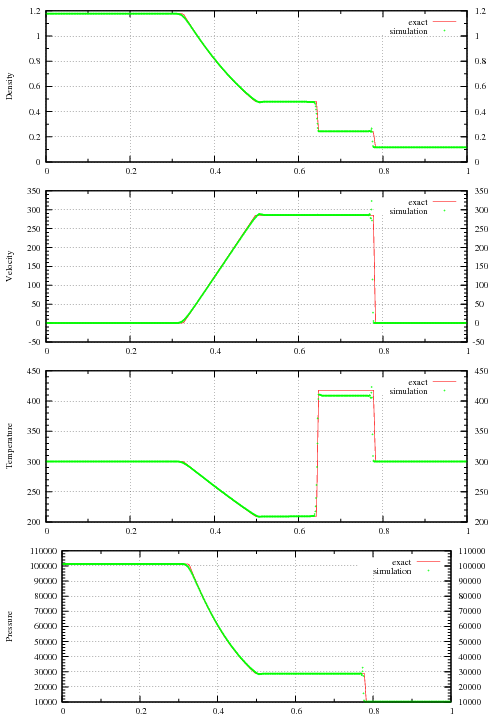
\includegraphics[scale=.85]{shockTube.png}
  \caption{Shock tube results at time $t = 5msec$}
  \label{results.ST}
  \end{figure}
\newpage

%__________________________________SHOCKTUBE AMR

\section*{\center Shock Tube with AMR}
 
\subsection*{\underline{Simulation Specifics}}
\begin{description} 
\footnotesize
\item [Component used:] \hfill ICE
\item [Input file name:] \hfill shocktube\_AMR.ups
\item [Command used to run input file:]\hfill sus inputs/UintahRelease/ICE/shocktube\_AMR.ups
\item [Postprocessing command:]\hfill \\
inputs/UintahRelease/ICE/plot\_shockTube\_AMR shockTube\_AMR.uda y
This will generate a postscript file shockTube\_AMR.ps

\item [Simulation Domain:]\hfill    1 x .001 x .001 m
\item [Cell Spacing:]\hfill 
10 x 1 x 1 mm (Level 0)\\
2.5 x 1 x1 mm (Level 1)\\
0.625 x1 x1 mm (Level 2)

\item [Example Runtimes:] \hfill \\
 2ish minutes   (1 processor, 2.66 GHz Xeon)

\item [Physical time simulated:] \hfill 0.005 sec.

\end{description}

\section*{\underline{Results}}
Figure \ref{results.ST.AMR} shows a comparison of the exact versus simulated results at time $t = 5msec$.
\begin{figure}
  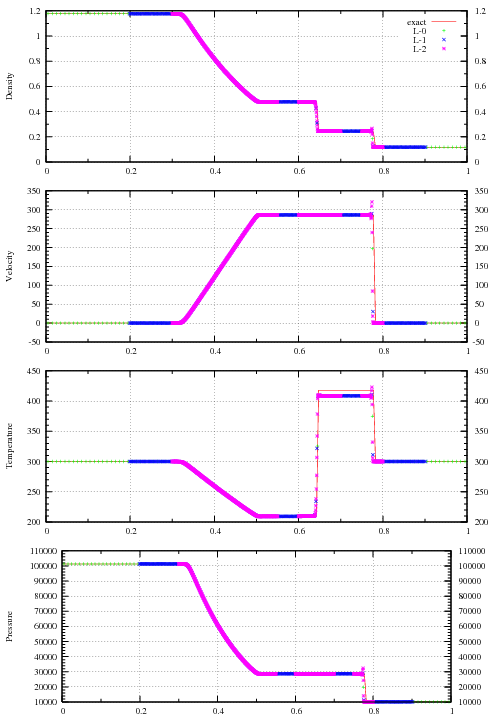
\includegraphics[scale=.85]{shockTube_AMR.png}
  \caption{Shock tube results at time $t = 5msec$}
  \label{results.ST.AMR}
  \end{figure}
\newpage

%__________________________________riemann2D

\section*{\center 2D Riemann Problem with AMR}
\subsection*{\underline{Problem Description}}
In two-dimensional Riemann problems there 15 different solutions that combine rarefaction waves, shock waves and a slip line or contact discontinuities \cite{ref:schulz_collins_glaz, ref:Liska_Wendroff}.  Here we simulate 4 slip lines that form a symmetrical single vortex turning counter clockwise. At time $t=0$ the computational domain is divided into four quadrants by the lines $x = 1/2, y=1/2$  The initial condition for $V=(p, \rho, u, v)$ in the four quadrants are $V_{ll}=(1, 1, -0.75, 0.5), V_{lr}=(1, 3, -0.75,-0.5), V_{ul}=(1,2,0.75,0.5), V_{ur}=(1,1,0.75,-0.5)$ where, $p$ is pressure, $\rho$ is the density of the polytropic gas, $u$ and $v$ are the $x$ and $y$ component of velocity.
\subsection*{\underline{Simulation Specifics}}
\begin{description} 
\footnotesize
\item [Component used:] \hfill ICE
\item [Input file name:] \hfill riemann2D\_AMR.ups
\item [Command used to run input file:]\hfill mpirun -np 5 sus inputs/UintahRelease/ICE/riemann2D\_AMR.ups
\item [VisIT session file:]\hfill inputs/UintahRelease/ICE/riemann2D.session
\item [Simulation Domain:]\hfill    0.96 x 0.96m x 0.1 m
\item [Cell Spacing:]\hfill \\ 
40  x 40  x 1 mm (Level 0)\\
10  x 10  x 1 mm (Level 1)\\
2.5 x 2.5 x 1 mm (Level 2)

\item [Example Runtimes:] \hfill \\
 5ish minutes   (5 processors, 2.66 GHz Xeon)
\item [Physical time simulated:] \hfill 0.3 sec.
\end{description}

\section*{\underline{Results}}
Figure \ref{fig:riemann2D} shows a flood and line contour plot(s) of the density of the gas at 0.03sec.
\begin{figure}
  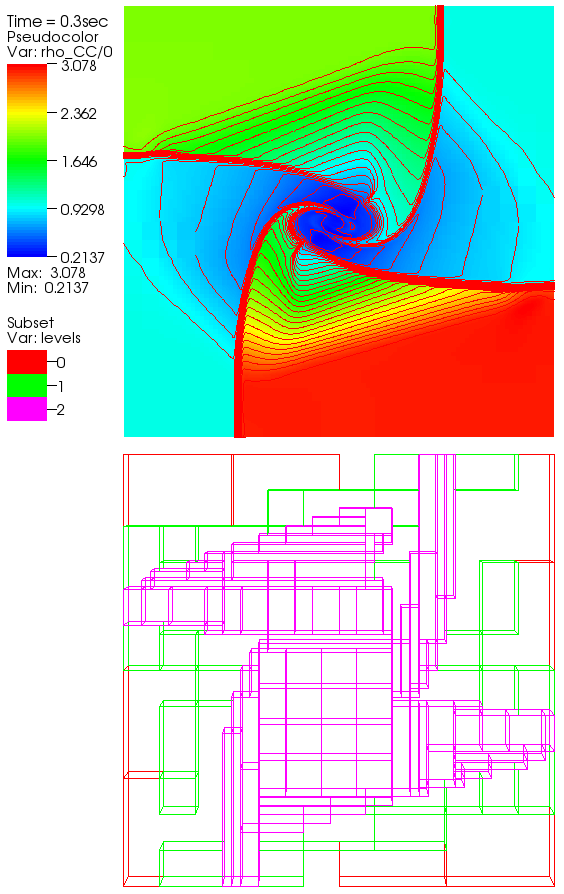
\includegraphics[scale=.6]{riemann2D.png}
  \caption{Contour plot of density for the 2D Riemann problem at time $t = 0.3sec$.  Bottom plot shows the outline of the patches on the 3 levels.}
  \label{fig:riemann2D}
  \end{figure}
\newpage

%__________________________________Single level blast wave

\section*{\center BlastWave 2D}
\subsection*{\underline{Problem Description}}
The Sedov-Taylor blastwave problem is a standard compressible flow problem
that has been used by many as a validation test case.  At time $t=0$ there
is a small region of gas at the center of the domain at a relatively high
temperature and pressure.  The expansion of high pressure gas forms a
spherical blast wave that expands into surrounding atmosphere.
\subsection*{\underline{Simulation Specifics}}
\begin{description} 
\item [Component used:] \hfill ICE
\item [Input file name:] \hfill blastWave.ups
\item [Command used to run input file:]\hfill sus blastWave.ups
\item [Visualization net file:]\hfill blastWave\_1L.srn\\


\item [Simulation Domain:]\hfill    1 x 1 x .05 m
\item [Cell Spacing:]\hfill \\ 
5 x 5 x 50 mm (Level 0)


\item [Example Runtimes:] \hfill \\
 9ish minutes   (1 processor, 2.66 GHz Xeon)

\item [Physical time simulated:] \hfill 0.9e-3sec.

\end{description}

\section*{\underline{Results}}
Figure \ref{results.BW} shows a comparison of the exact versus simulated
results at time $t = 5msec$.

\begin{figure}
  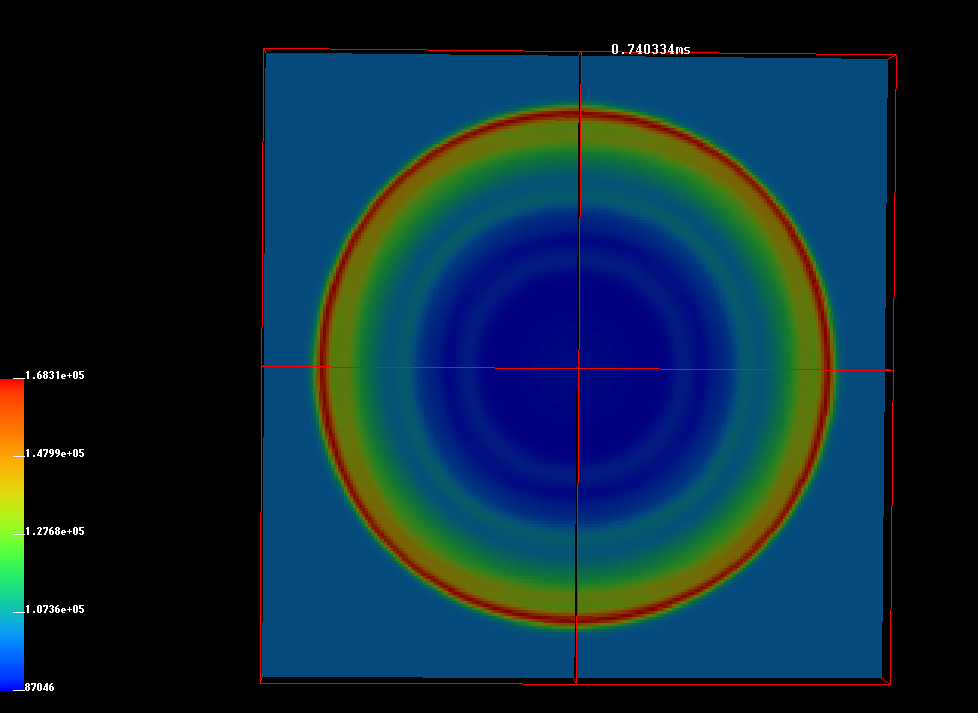
\includegraphics[scale=.5]{blastWave.png}
  \caption{Pressure field at time $t = 0.74msec$}
  \label{results.BW}
  \end{figure}
\newpage

%__________________________________AMR blast wave

\section*{\center BlastWave AMR}
\subsection*{\underline{Simulation Specifics}}
\begin{description} 
\item [Component used:] \hfill ICE
\item [Input file name:] \hfill blastWave.ups
\item [Command used to run input file:]\hfill sus blastWave\_AMR.ups
\item [Visualization net file:]\hfill blastWave\_1L.srn\\


\item [Simulation Domain:]\hfill    1 x 1 x .05 m
\item [Cell Spacing:]\hfill \\ 
20 x 20 x 50 mm (Level 0) 
5 x 5 x 50 mm (Level 1)


\item [Example Runtimes:] \hfill \\
 9ish minutes   (1 processor, 2.66 GHz Xeon)

\item [Physical time simulated:] \hfill 0.9e-3sec.

\end{description}

\section*{\underline{Results}}
Figure \ref{results.BW.AMR} shows the pressure field and an outline of the
individual patches on levels 0 \& 1.  This simulation shows the adaptive
mesh capabilities of ICE and the UCF.
\begin{figure}
  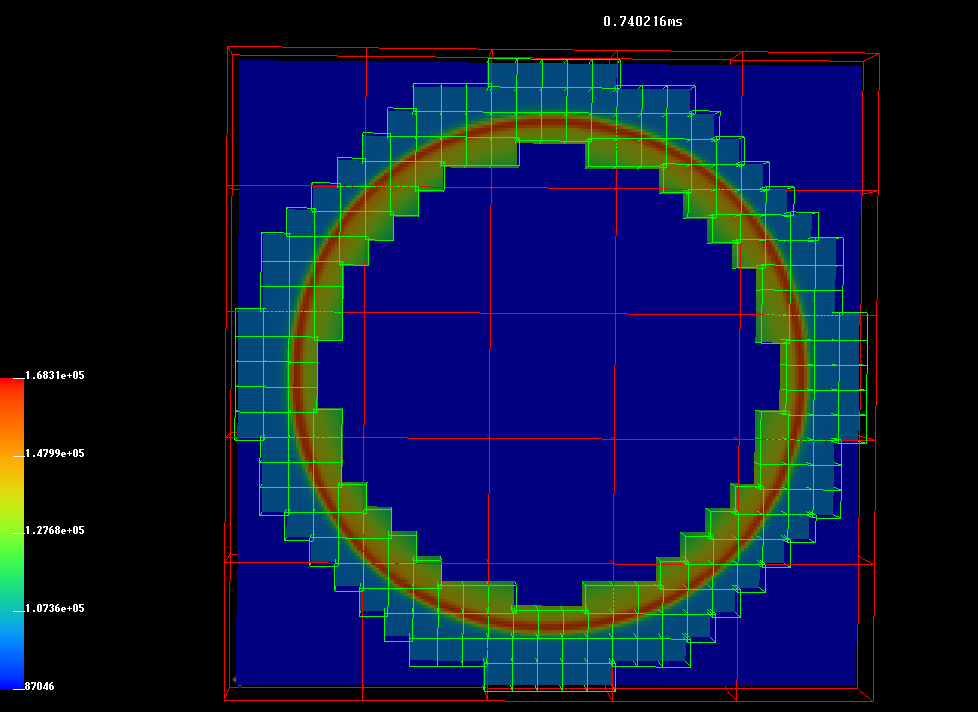
\includegraphics[scale=.5]{blastWave_AMR.png}
  \caption{Pressure field at time $t = 0.74msec$.  The individual patches on levels 0 \& 1 are shown.}
  \label{results.BW.AMR}
  \end{figure}
Good agreement between the single level results (Fig. \ref{results.BW}) and the AMR results (Fig.
\ref{results.BW.AMR}) is shown.
\newpage

%__________________________________CH4 fire

\section*{\center Methane Flame}
\subsection*{\underline{Problem Description}}
At $t=0$ Methane gas begin flowing from a $1m$ hole in the floor of the
computational domain at a velocity of $1m/s$.  The methane mixes with the
surrounding air, ignites and forms a puffing fire.  The main assumptions in
this simulation are a) that the chemical reactions are taking place infinitely
fast (equilibrium chemistry model) and b) that there is no radiative heat
loss from the product gases.
\subsection*{\underline{Simulation Specifics}}
\begin{description} 
\item [Component used:] \hfill ICE
\item [Input file name:] \hfill CH4\_fire.ups
\item [Command used to run input file:]\hfill sus CH4\_fire.ups \\
Note you must have a link to the {\tt inputs} directory in the save directory as sus.  A table needed
by the combustion model is inside the {\tt inputs} directory.
\item [SCIRun visualization net file:]\hfill 3DFire\_Vol.srn \\


\item [Simulation Domain:]\hfill    5 x 5 x 5 m
\item [Cell Spacing:]\hfill \\ 
3.3 x 3.3 x 3.3 cm (Level 0)


\item [Example Runtimes:] \hfill \\
 8 hours   (64 processor, 2.66 GHz Xeon)

\item [Physical time simulated:] \hfill 3.4sec.

\end{description}

\section*{\underline{Results}}
Figure \ref{results.CH4} shows a 3D view of the initial puff just before it leaves the computational
doman.  
\begin{figure}
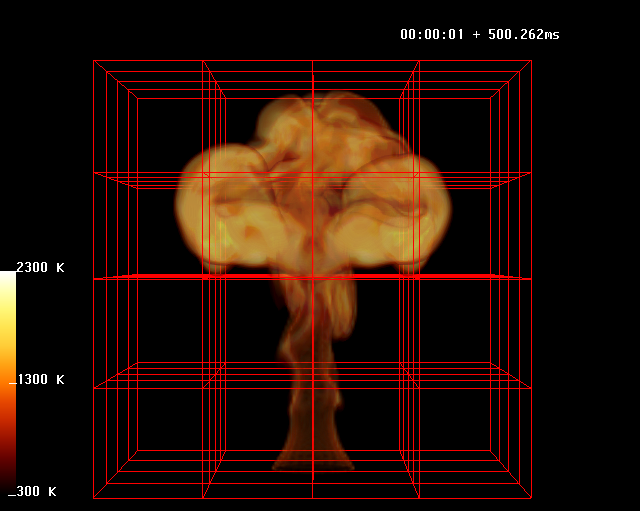
\includegraphics[scale=.66]{3DFire.png}
\caption{Temperature field at time $t = 1.5 sec$}
\label{results.CH4}
\end{figure}
\newpage


\subsection{References}
\bibliographystyle{plain}
\bibliography{ice}




\section{MPM}

\subsection{Introduction}

\subsection{Theory - Algorithm Description}

\subsection{Uintah Specification}

\subsubsection{Basic Inputs}
\subsubsection{Physical Constants}
\subsubsection{Material Properties}
\subsubsection{Constitutive Models}
\subsubsection{Contact}
\subsubsection{BoundaryConditions}
\subsubsection{Physical Boundary Conditions}

\subsection{Examples}

\subsection{References}

%
\section{MPMArches}

\subsection{Introduction}

\subsection{Theory - Algorithm Description}

\subsection{Uintah Specification}

\subsubsection{Arches}

\subsubsection{Basic Inputs}
\subsubsection{Turbulence}
\subsubsection{Properties}
\subsubsection{BoundaryConditions}
\subsubsection{Physical Constants}
\subsubsection{Solvers}


\subsubsection{MPM}

\subsubsection{Basic Inputs}
\subsubsection{Physical Constants}
\subsubsection{Material Properties}
\subsubsection{Constitutive Models}
\subsubsection{Contact}
\subsubsection{BoundaryConditions}
\subsubsection{Physical Boundary Conditions}

\subsection{Examples}

\subsection{References}


\chapter{MPMICE} \label{Sec:MPMICE}

\section{Introduction}

MPMICE is a marriage of the multi-material ICE method, described in
Section~\ref{Sec:ICE} and MPM, described in Section~\ref{Sec:MPM}.
The equations of motion solved for both fluid and solid are essentially
the same, although the physical behavior of these two states of matter
differ, largely due to their constitutive relationships.  MPM is used
to track the evolution of solid materials in a Lagrangian frame of
reference, while fluids are evolved in the Eulerian frame.

\section{Theory - Algorithm Description}

At this time, the reader is directed to the manuscript by Guilkey,
Harman and Banerjee~\cite{fourthmit} for the theoretical and algorithmic
description of the method.

%\subsection{Uintah Specification}

%\subsubsection{ICE}

%\subsubsection{Basic Inputs}
%\subsubsection{Physical Constants}
%\subsubsection{Material Properties}
%\subsubsection{Equation of State}
%\subsubsection{Exchange Properties}
%\subsubsection{BoundaryConditions}
%\subsubsection{Solvers}


%\subsection{MPM}

%\subsubsection{Basic Inputs}
%\subsubsection{Physical Constants}
%\subsubsection{Material Properties}
%\subsubsection{Constitutive Models}
%\subsubsection{Contact}
%\subsubsection{BoundaryConditions}
%\subsubsection{Physical Boundary Conditions}

\section{HE Combustion Models}

Three models exist for reaction of high explosive materials.  Each simulation using one of these models utilize MPMICE's material interactions as its foundation.  The components work by taking several material specific constants as well as a reactant and product material from the model input section of the .UPS file.  Following are brief descriptions of each model, as well as their input parameters.

\subsection{Simple Burn} \label{Sec:SimpleBurn}

Simple Burn, as the name implies, is a simple model of combustion of HMX based on the rate equation:

\begin{equation}
\dot{m}=A P^{0.778}
\label{simburneqn}
\end{equation}

Where $\dot{m}$ is the mass flux, $P$ is the pressure and $n$ is the pressure dependence coefficient.  The pressure coefficient in Equation (\ref{simburneqn}) is that of HMX.  The models input section for a Simple Burn simulation takes the form: 

\begin{verbatim}
<Models>
  <Model type="Simple_Burn">
    <fromMaterial> reactant      </fromMaterial>
    <toMaterial>   product       </toMaterial>
    <Active>       true          </Active>
    <ThresholdTemp>       450.0  </ThresholdTemp>
    <ThresholdPressure> 50000.0  </ThresholdPressure>
    <Enthalpy>        2000000.0  </Enthalpy>
    <BurnCoeff>            75.3  </BurnCoeff>
    <refPressure>      101325.0  </refPressure>
  </Model>
</Models>
\end{verbatim}

The first two tags take names of materials previously defined in the input file, defining both reactant and product used by the model.  See Section \ref{sec:ICEmat_props} and \ref{mat_props} for in depth description for defining materials.  $<$Active$>$ is a debugging parameter that takes a boolean value indicating whether the model is on (i.e. the actual computations take place during the timestep).  True is the value to set for $<$Active$>$ in most situations.  Each of the other parameters take double values.  Threshold temperature and pressure tags define two criteria the cell must have in order to be flagged burning.  The reference pressure is used to scale the cell centered pressure as well as make it an unitless value.  The burn coefficient corresponds to $A$ in the rate equation.  Enthalpy is simply the enthalpy value for conversion of reactant to product.
\newpage
\subsection{Steady Burn} \label{Sec:SteadyBurn}

Steady Burn is a more accurate model than Simple Burn.  It is based on WSB model of combustion developed by Ward, Son and Brewster in \cite{ref:wardsonbrewster}.  WSB is based on a simplified two-step chemical model with an initial zero-order, thermally activated ($E_c > 0$), mildly exothermic, solid-to-gas reaction, modeled as a thermal decomposition of the solid:

\begin{equation}
A(solid)\rightarrow B(gas)
\end{equation}

Intermediate $B$, in the presence of any gas phase collision partner $M$, reacts in a highly exothermic fashion producing a flame.  This step is modelled as a second-order, gas phase, free radical chain reaction based on the assumption that $E_g = 0$:

\begin{equation}
B(gas)+M(gas)\rightarrow C(gas)+M(gas)
\end{equation}

As such, this second equation represents the reaction in the gas phase that causes heat convection back to the surface that activate the first reaction.  In Steady Burn, a solution is found by iteratively solving two equations: one for mass burning rate $\dot{m}$ and one for surface temperature $T_s$.  Mass flux is initially solved with an assumed value $T_s$ (in the model set to $850.0 K$) using WSB:

\begin{equation}
\dot{m}\left(T_s\right)=\sqrt{\frac{\displaystyle \kappa_c \rho_c A_c R T_s^2 \exp\left({\frac{\displaystyle -E_c}{\displaystyle R T_s}}\right)}{\displaystyle C_p E_c \left(T_s - T_0 - \frac{Q_c}{2 C_p}\right)}}
\label{WSB1}
\end{equation}

The solution to this equation is used to refine the surface temperature and vice-versus until a self-consistent solution for surface temperature and mass flux has been found.  The surface temperature equation takes the form:

\begin{equation}
T_s(\dot{m},P)=T_0 + \frac{\displaystyle Q_c}{\displaystyle C_p} + \frac{Q_g}{Cp\left(1+\frac{\displaystyle x_g\left(\dot{m},P\right)}{\displaystyle x_{cd}(\dot{m})}\right)}
\label{WSB2}
\end{equation}

$x_g$ in the third term of Equation (\ref{WSB2}) is the flame standoff distance, computed from:

\begin{equation}
x_g\left(\dot{m},P\right)=\frac{2 x_{cd}\left(\dot{m}\right)}{\displaystyle \sqrt{1 + D_a\left(\dot{m},P\right)} - 1}
\label{WSB3}
\end{equation}

where $x_{cd}$ and $D_a$ are the convective-diffusive length and Damkohler number, respectively:

\begin{equation}
x_{cd} \left(\dot{m}\right)=\frac{\kappa_g}{\displaystyle \dot{m} C_p}
\label{WSB4}
\end{equation}
\begin{equation}
D_a\left(\dot{m},P\right) = \frac{4 B_g M C_p P^2}{\displaystyle R^2 \kappa_g} x_{cd}\left(\dot{m}\right)^2
\label{WSB5}
\end{equation}

WSB model is valid as a 1D model, but needs extension to work in a 3D multimaterial CFD environment.  As such, Steady Burn is WSB extended with logic for ignition of energetic materials and computation of surface area for burning cells.  Ignition of a cell is based on three criteria: 
\begin{itemize}
  \item The cell must contain one particle of energetic solid
  \item The cell is near a surface of an energetic solid (e.g. ratio of minimum node-centered mass to maximum node-centered mass is less than 0.7)
  \item One neighboring cell must have at most two particles of energetic material
\end{itemize}
If a cell is ignited, the model will be applied and mass will be transferred from reactant material to product material.  Total mass burned is computed using mass flux $\dot{m}$, $\Delta t$ of the timestep and the calculated surface area, found using:

\begin{equation}
A=\frac{\delta x \delta y \delta z}{\displaystyle \delta x |g_x| + \delta y |g_y| + \delta z |g_z|}
\label{WSB6}
\end{equation} where $\delta x$, $\delta y$, and $\delta z$ are the dimensions of the cell and components of $\overrightarrow{g}$ are the normalized density gradients of the particle mass in a cell.  A more thorough examination of Steady Burn can be read about in \cite{ref:wighteddings}.

The following table describes the input parameters for Steady Burn.  The final column of the table indicates parameters for combustion of HMX.  

\begin{center}
\begin{tabular}{| l | c | p{4cm} | l |}
\hline
  \multicolumn{4}{|c|}{\textbf{Steady Burn Input Parameters}} \\
\hline
\hline
  \textbf{Tag} & \textbf{Type} & \textbf{Description} & \textbf{HMX Value} \\
\hline
  $<$fromMaterial$>$ & String & 'Name' of reactant material (mass source) &  \\
\hline
  $<$toMaterial$>$ & String & 'Name' of product material (mass sink) & \\
\hline
  $<$IdealGasConst$>$ & double & Ideal gas constant ($R$) & $8.314 J/(K\times mol)$ \\
\hline
  $<$PreExpCondPh$>$ & double & Condensed phase pre-exponential coefficient ($A_c$) & $1.637\times10^{15} s^{-1}$ \\
\hline
  $<$ActEnergyCondPh$>$ & double & Condensed phase activation energy ($E_c$) & $1.76\times10^5 J/mol$ \\
\hline
  $<$PreExpGasPh$>$ & double & Gas phase frequency factor ($B_g$) & $1.6\times10^{-3} m^3/(kg\times s\times K)$ \\
\hline
  $<$CondPhaseHeat$>$ & double & Condensed phase heat release per unit mass ($Q_c$) & $4.0\times10^5 J/kg$ \\
\hline
  $<$GasPhaseHeat$>$ & double & Gas phase heat release per unit mass ($Q_g$) & $3.018\times10^6 J/kg$ \\
\hline
  $<$HeatConductGasPh$>$ & double & Thermal conductivity of gas ($\kappa_g$) & $0.07 W/(m\times K)$ \\
\hline
  $<$HeatConductCondPh$>$ & double & Thermal conductivity of condensed phase ($\kappa_c$) & $0.02 W/(m\times K)$ \\
\hline
  $<$SpecificHeatBoth$>$ & double & Specific heat at constant pressure ($c_p$) & $1.4\times10^3 J/(kg\times K)$ \\
\hline
  $<$MoleWeightGasPh$>$ & double & Molecular weight of gas ($W$) & $3.42\times10^{-2} kg/mol$ \\
\hline
  $<$BoundaryParticles$>$ & int & Max \# of particles a cell can have and be burning & Resolution dependent \\
\hline
  $<$ThresholdPressure$>$ & double & Threshold pressure cell must have $\ge$ to burn mass & $50000 Pa$ \\
\hline
  $<$IgnitionTemp$>$ & double & Temperature cell must have $\ge$ to be burning & $550 K$ \\
\hline
\end{tabular}
\end{center}

\newpage
\subsection{Unsteady Burn} \label {Sec:UnsteadyBurn}

Unsteady Burn is a model developed at the University of Utah as an extension of Steady Burn to better represent mass burning rates when pressure at the burning surface fluctuates. A pressure-coupled response is accounted for in the model such that, qualitatively a pressure increase causes gas phase reaction rates to increase as well as move the gas phase reactions closer to the burning surface.  Increase of near surface gas phase reactions increases the rate of thermally activated solid state reactions, ultimately causing a higher steady burn rate.  Unsteady Burn more accurately models the transition from low pressure to high pressure than Steady Burn by taking into account the initially overshot burn rate at the time when the pressure increases, and the relaxation period to steady burn rate.  Similarly, Unsteady Burn models undershot pressures during pressure drops.  

The model is an extension of Steady Burn by partial decoupling of the gas phase and solid state Equations (\ref{WSB1}) and (\ref{WSB2}).  An expression for the temperature gradient of the solid:

\begin{equation}
  \beta = \left(T_s - T_0\right) \frac{m c_p}{\displaystyle\kappa_c}
  \label{WSB7}
\end{equation}

is reaarranged for $(T_s-T_0)$ and substituted in Equation (\ref{WSB1}) leading to the quadradic equation:

\begin{equation}
\dot{m}^2 - \frac{2 \beta \kappa_c}{Q_c} \dot{m} + \frac{2 A_c R T_s^2 \kappa_c \rho_c }{E_c Q_C} \exp\left({\frac{-E_c}{R T_s}}\right)=0
\label{WSB8}
\end{equation}

which allows independent tracking of temperature gradient $\beta$ and surface temperature $T_s$.  The gas phase response is computed using a runnning average of $T_s$ as it approaches the steady burning value.  A solid state response is obtained by computing a running average of $\beta$ as it approaches the steady burning value.  A slow relaxation time for $\beta$ and a fast relaxation time for $T_s$ models the overshoot or undershoot in burn rate.  Burning criteria for a cell is the same as Steady Burn.  For more information on Unsteady Burn see \cite{ref:wighteddings}.

The following table describes the input parameters for Unsteady Burn.

\begin{center}
\begin{tabular}{| l | c | p{7cm} |}
\hline  
  \multicolumn{3}{|c|}{\textbf{Unsteady Burn Input Parameters}} \\
\hline
\hline
  \textbf{Tag} & \textbf{Type} & \textbf{Description}\\
\hline
  $<$fromMaterial$>$ & String & 'Name' of reactant material (mass source)\\
\hline
  $<$toMaterial$>$ & String & 'Name' of product material (mass sink)\\
\hline
  $<$IdealGasConst$>$ & double & Ideal gas constant ($R$)\\
\hline
  $<$PreExpCondPh$>$ & double & Condensed phase pre-exponential coefficient ($A_c$) \\
\hline
  $<$ActEnergyCondPh$>$ & double & Condensed phase activation energy ($E_c$)\\
\hline
  $<$PreExpGasPh$>$ & double & Gas phase frequency factor ($B_g$)\\
\hline
  $<$CondPhaseHeat$>$ & double & Condensed phase heat release per unit mass ($Q_c$)\\
\hline
  $<$GasPhaseHeat$>$ & double & Gas phase heat release per unit mass ($Q_g$)\\
\hline
  $<$HeatConductGasPh$>$ & double & Thermal conductivity of gas ($\kappa_g$)\\
\hline
  $<$HeatConductCondPh$>$ & double & Thermal conductivity of condensed phase ($\kappa_c$)\\
\hline
  $<$SpecificHeatBoth$>$ & double & Specific heat at constant pressure ($c_p$)\\
\hline
  $<$MoleWeightGasPh$>$ & double & Molecular weight of gas ($W$)\\
\hline
  $<$BoundaryParticles$>$ & int & Max \# of particles a cell can have and be burning\\
\hline
  $<$BurnrateModCoef$>$ & double & not sure... \\
\hline
  $<$CondUnsteadyCoef$>$ & double & not sure... \\
\hline
  $<$ThresholdPressure$>$ & double & Threshold pressure cell must be $\ge$ to burn mass\\
\hline
  $<$IgnitionTemp$>$ & double & Temperature cell must be at $\ge$ to be burning\\
\hline
\end{tabular}
\end{center}

\newpage

\section{Examples} \label {Sec:MPMICE_EXAMPLES}

\subsection*{\center Mach 2 Wedge}
\addcontentsline{toc}{subsection}{Mach 2 Wedge}
\subsubsection*{\underline{Problem Description}}
This is a simulation of a symmetric $20^o$ wedge traveling through initially
quiescent air at Mach 2.0.  A shock forms at the leading edge of the
wedge and an expansion fan over its top.  Consultation of oblique shock
tables, e.g.~\cite{ref:Saad} (pp.308-309) reveals that the angle of the leading
shock compares quite well with the expected value.  In addition, this
simulation demonstrates a few other useful features of the fluid-structure
interaction capability.  In this case, the structure is rigid, and as
such, essentially provides a boundary condition to the compressible flow
calculation.  Furthermore, the geometry of the wedge is described via a
triangulated surface, rather than the geometric primitives usually used.
This allows the user to study flow around arbitrarily complex objects,
without the difficulty of generating a body fitted mesh around that object.

\subsubsection*{\underline{Simulation Specifics}}
\begin{description}
\item [Component used:] \hfill rmpmice (Rigid MPM-ICE)
\item [Input file name:] \hfill Mach2Wedge.ups
\item [Command used to run input file:]\hfill sus Mach2Wedge.ups
(Note: The files wedge40.pts and wedge40.tri must also be copied to
the same directory as sus.)

\item [Simulation Domain:]\hfill    0.25 x 0.0375 x 0.001 m

\item [Cell Spacing:]\hfill \\
.0005 x .0005 x .001 m (Level 0)

\item [Example Runtimes:] \hfill \\
 20 minutes   (1 processor, 3.16 GHz Xeon)\\

\item [Physical time simulated:] \hfill 0.3 milliseconds

\item [Associated visit session:] \hfill M2wedge.session

\end{description}

\newpage

\subsubsection*{\underline{Results}}

Figure~\ref{figwedge} shows a snapshot of the simulation.  Contour
plot depicts pressure and reflects the presence of a leading shock
and an expansion fan.
\begin{figure}
  \center
  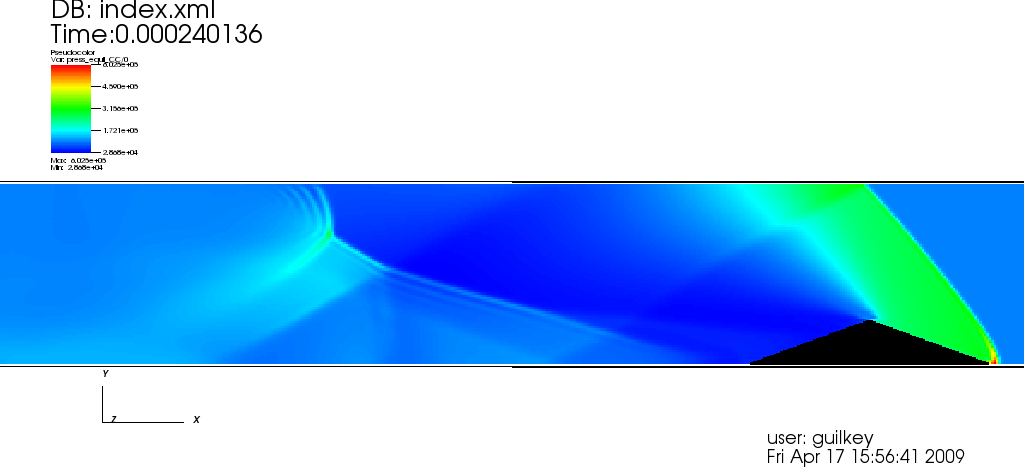
\includegraphics[scale=.4]{M2wedge.png}

  \caption{$20^o$ wedge moving at Mach 2.0 through initially stationary
air.  Contour plot depicts pressure.}
  \label{figwedge}
\end{figure}
\newpage
%
%__________________________________
\subsection*{\center Cylinder in a Crossflow}
\addcontentsline{toc}{subsection}{Cylinder in a Crossflow}
\subsubsection*{\underline{Problem Description}}
In this example the domain is initially filled with air moving at a uniform velocity of $0.03m/s$  A ridgid cylinder $O.D. = 0.02m$ is placed $0.1m$ from the inlet and a passive scalar is injected into the domain through a $0.002m$ hole on in the inlet boundary of the domain.  A velocity perturbation is placed upstream of the cylinder to produce an instablity that will help trigger the onset of the K\'arm\'an vortex street.
%
\subsection*{\underline{Simulation Specifics}}
\begin{description}
\item [Component used:] \hfill rmpmice (Rigid MPM-ICE)
\item [Input file name:] \hfill \TT{cylinderCrossFlow.ups}
\item [Command used to run input file:]\hfill \\
\TT{mpirun -np 6  sus inputs/UintahRelease/MPMICE/cylinderCrossFlow.ups}

\item [Simulation Domain:]\hfill    0.3 x 0.15 x 0.001 m

\item [Cell Spacing:]\hfill \\
.00015 x .001 x .001 m (Level 0)

\item [Example Runtimes:] \hfill \\
 7ish hrs   (6 processor, 3.16 GHz Xeon)\\

\item [Physical time simulated:] \hfill 60 seconds

\item [Associated visit session:] \hfill cyl\_crossFlow.session

\end{description}

\section*{\underline{Results}}

Figure~\ref{fig:cylCrossFlow} shows a snapshot of the simulation at time $t=60sec$.  The contour
plot of the passive scalar shows the K\'arm\'an vortex street behind the cylinder at $Re=700$.
\begin{figure}
  \center
  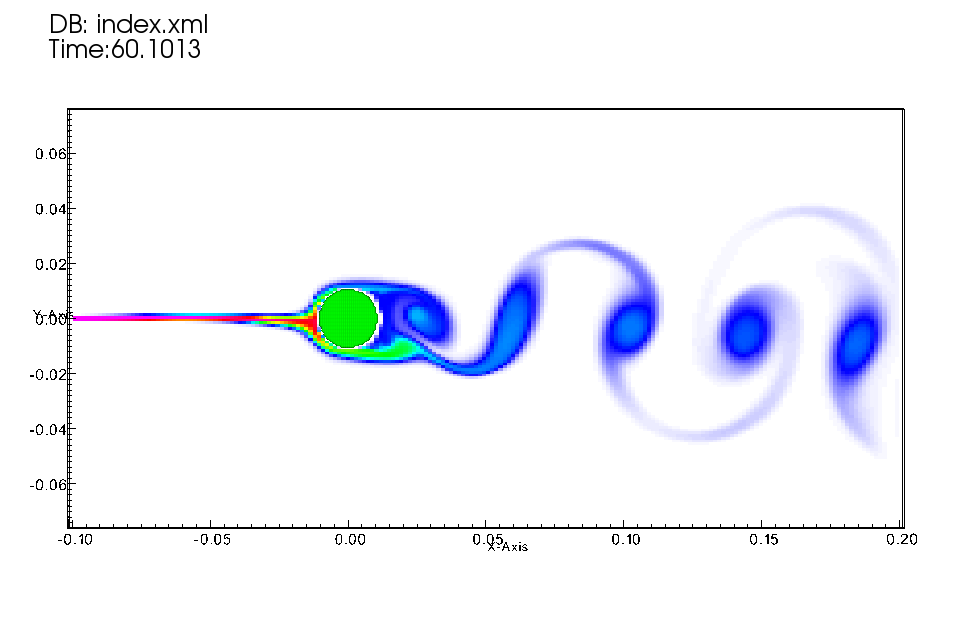
\includegraphics[scale=.5]{cylCrossFlow.png}
  \caption{Flow over a stationary cylinder, $Re=700$, a passive scalar is used as a flow marker}
  \label{fig:cylCrossFlow}
\end{figure}
%
A movie of the results is located at
\begin{Verbatim}[fontsize=\footnotesize]
  movies/cyl_crossFlow.mpg
\end{Verbatim}
\newpage

%__________________________________
\subsection*{\center Copper Clad Rate Stick (aka ``Cylinder Test")}
\addcontentsline{toc}{subsection}{"Cylinder Test"}
\subsubsection*{\underline{Problem Description}}

This is a two-dimensional version of the ``cylinder test" which is used to
characterize equations of state for explosive products.  In those tests, a
copper tube is filled with a high explosive and a detonation is initiated
at one end.  Various means are used to measure the velocity of the tube as
the high pressure product gases expand inside of it.

Here, a cylinder ($r=2.54 cm$) of QM100 is jacketed with a copper cylinder
that has a wall thickness of $0.52 cm.$   Detonation is initiated by giving
a thin layer of the explosive a high initial velocity in the axial direction
which generates a pressure that is sufficiently high to reach trigger the
detonation model.  As the detonation proceeds, the copper is pushed out of
the domain by the expanding product gases.

Note that in this example, to make run times brief, the domain is very short
in the axial direction, and is probably not sufficient for the detonation to
reach steady state.  Additionally, the domain has been reduced to two
dimensions, as symmetry is assumed in the Z-plane.  Finally, the spatial
resolution of $1.0 mm$ is a bit coarse to achieve 
convergent results.  The full three dimensional result can quickly be
obtained by commenting out the symmetry condition on the z+ plane and
uncommenting the Neumann conditions, as well as changing the spatial extents
and resolution in the Z direction to match those in the Y direction.

%
\subsubsection*{\underline{Simulation Specifics}}
\begin{description}
\item [Component used:] \hfill mpmice (MPM-ICE)
\item [Input file name:] \hfill \TT{QM100CuRS.ups}
\item [Command used to run input file:]\hfill \\
\TT{sus inputs/UintahRelease/MPMICE/QM100CuRS.ups}

\item [Simulation Domain:]\hfill    0.055 x 0.032 x 0.0005 m

\item [Cell Spacing:]\hfill \\
1.0 mm x 1.0 mm x 1.0 mm (Level 0)

\item [Example Runtimes:] \hfill \\
 20 minutes   (1 processor, 3.16 GHz Xeon)\\

\item [Physical time simulated:] \hfill 30 $\mu$seconds

\item [Associated visit session:] \hfill QM100.session

\end{description}

\subsubsection*{\underline{Results}}

Figure~\ref{fig:QM100} shows a snapshot of the simulation at time $t=60sec$.
Particles are colored by velocity magnitude, contours reflect the density of
explosive, note the highly compressed region near the shock front.
\begin{figure}
  \center
  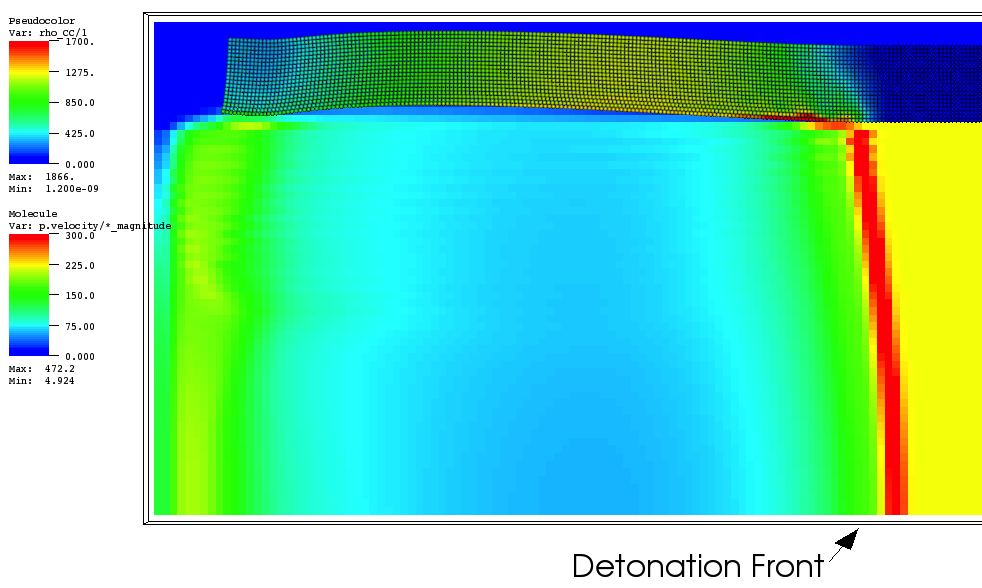
\includegraphics[scale=.5]{QM100.png}
  \caption{Detonation in a copper cylinder (2-D).  Particles are colored by
           velocity magnitude, contours indicate density of unreacted
           explosive.}
  \label{fig:QM100}
\end{figure}
%
\newpage

%________________
\section*{\center  Cylinder Pressurization Using Simple Burn}
\addcontentsline{toc}{subsection}{Cylinder Pressurization Using Simple Burn}
\subsection*{\underline{Problem Description}}
This example demonstrates use of the Simple Burn algorithm in an explosive scenario.  
The exact situation consists of a cylinder of PBX encased in steel.  For simplicity it is set up 
as a 2D simulation.  It demonstrates Symmetric boundaries as a useful construct for simplifying
the computational requirements of a problem.  The end result is the pressurization of a quarter
of a cylinder by combustion of PBX 9501.  Damage and failure models simulate cylinder failure
in a detonation scenario.  The simulation as it stands falls far short of the required physical time 
simulated for actual detonation, but demonstrates how Simple Burn can be used to pressurize 
a cylinder.  For description of Simple Burn see \ref{Sec:SimpleBurn}.

\subsection*{\underline{Simulation Specifics}}
\begin{description}
\item [Component used:] \hfill mpmice (MPM-ICE)
\item [Input file name:] \hfill guni2dRT.ups
\item [Preprocessing on input file:]\hfill \\ 1) Comment out or remove $<$max\_Timesteps$>$ on line 21 \\
2) Comment out $<$outputTimestepInterval$>$ on line 96 \\ 
3) add $<$outputInterval$>$5e-5$<$outputInterval$>$ on line 97 \\
\item [Command used to run input file:]\hfill mpirun -np 4 sus guni2dRT.ups

\item [Simulation Domain:]\hfill    8.636 x 8.636 x 0.16933 cm

\item [Example Runtimes:] \hfill \\
2 minutes   (1 processor, 2.8 GHz Xeon)\\

\item [Physical time simulated:] \hfill 8 microseconds \\ 


\item [Associated visit session:] \hfill SimpleBurn.session

\end{description}

\newpage

\section*{\underline{Results}}
With the recession of mass comes a pressure increase that causes the case to expand outward. 
A snapshot of pressure after the 0.4 milliseconds can be seen in Figure~\ref{figsimburn1}.  At this time
pressure has increased to three-fold its initial value.  A later snapshot Figure~\ref{figsimburn2} shows
the response of the steel cylinder to increased pressure.  Note that mass flux will scale according
to \ref{simburneqn}.  Another interesting view of the simulation can be seen in Figure~\ref{figsimburn3}.
On the left is the normal particle and pseudocolor map representing solid mass and pressure respectively.
On the top right, change in pressure during the timestep can be seen (delP\_Dilatate).  The bottom shows
change in pressure due to mass exchange (del\_MassX).  See table \ref{table:iceLabels} for description of
these variables.


\begin{figure}
  \center
  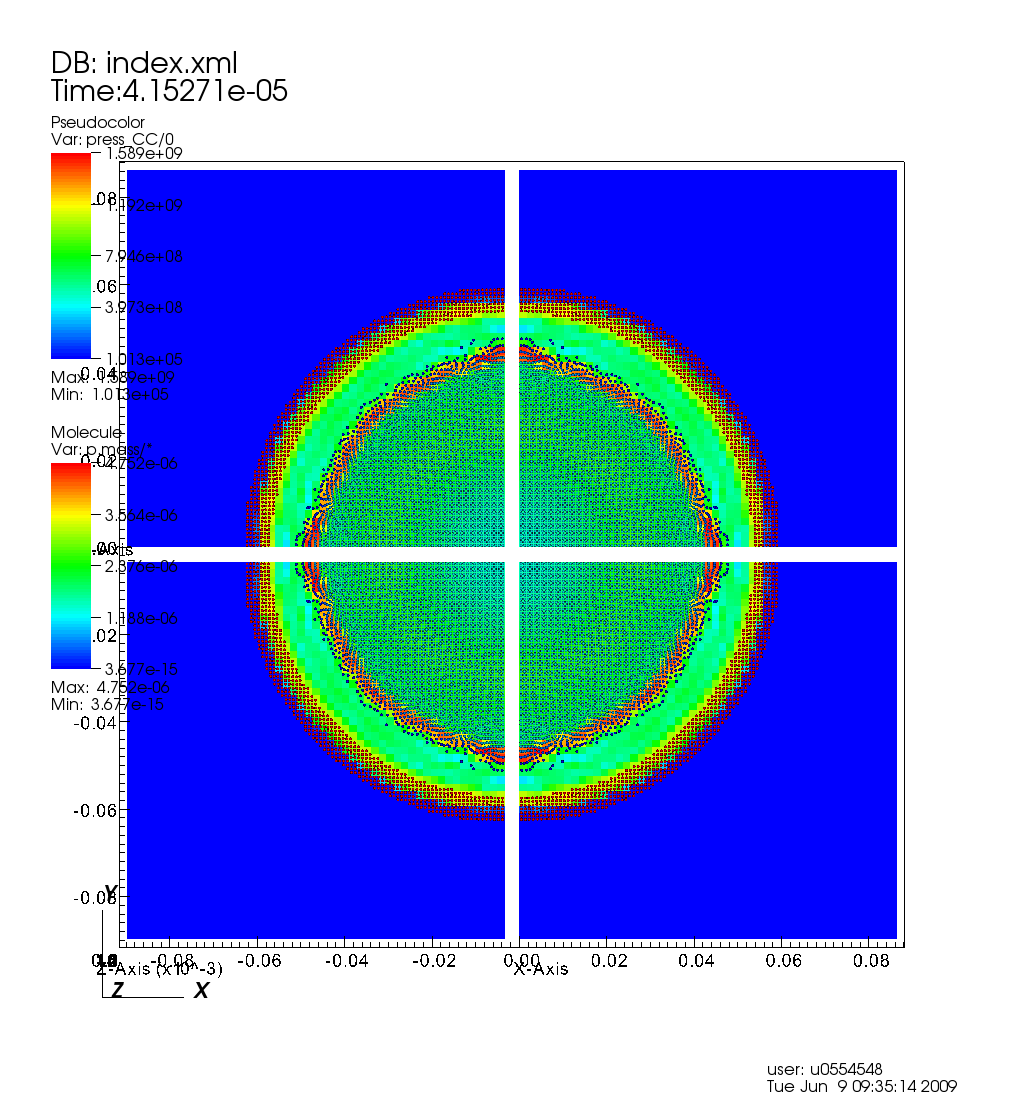
\includegraphics[scale=.3]{SimpleBurn0000.png}

  \caption{Receding PBX9501 leads to pressure increase in cylinder.}
  \label{figsimburn1}
\end{figure}

\begin{figure}
  \center
  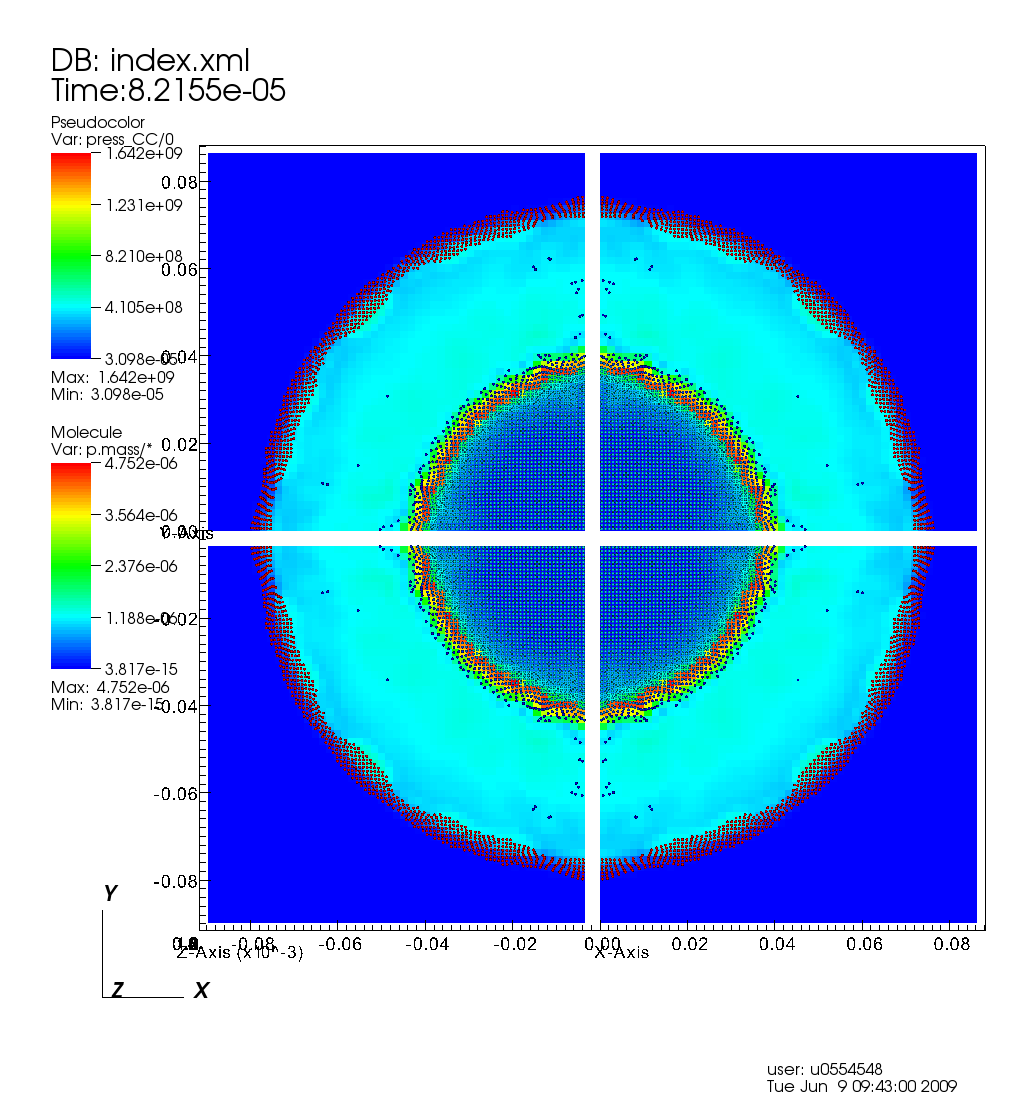
\includegraphics[scale=.3]{SimpleBurn0001.png}

  \caption{Pressure increase causes cylinder to respond.}
  \label{figsimburn2}
\end{figure}

\begin{figure}
  \center
  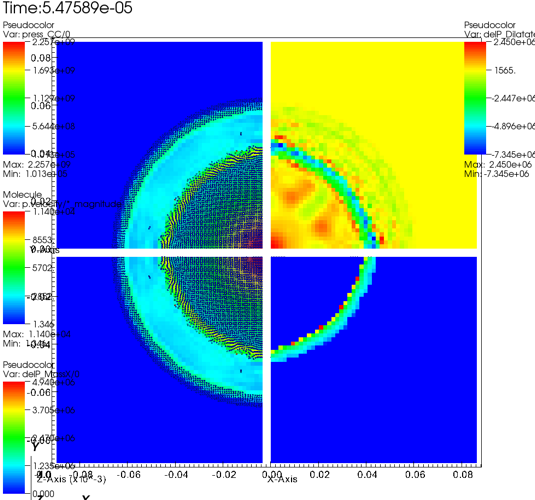
\includegraphics[scale=.3]{SimpleBurn0002.png}

  \caption{The left half of the image represents particles as spheres colored according to mass and pressure as background color.  Top-right shows delP\_Dilatate and bottom-right shows delP\_MassX.}
  \label{figsimburn3}
\end{figure}

\newpage


%
\section*{\center Exploding Cylinder Using Steady Burn}
\addcontentsline{toc}{subsection}{Exploding Cylinder Using Steady Burn}
\subsection*{\underline{Problem Description}}
This problem consistes of a cylinder initially at 600 K causing burning.  Steady Burn acts as the model for burning of HE material.  More information on Steady Burn can be found in \ref{Sec:SteadyBurn}.  The cylinder is build from an outer shell of steel covering a hollow bored cylinder of PBX9501.  The simulation demonstrates the violence of explosions when large voids allow rapid expansion of surface area due to collapse of explosive material into the bore.  Information on the violence of explosions with solid and hollow cores can be attained in \cite{ref:wighteddings}.  

\subsection*{\underline{Simulation Specifics}}
\begin{description}
\item [Component used:] \hfill mpmice (MPM-ICE)
\item [Input file name:] \hfill SteadyBurn\_2dRT.ups
\item [Preprocessing on input file:]\hfill \\ 1) Comment out or remove $<$max\_Timesteps$>$ \\ 2) Comment out $<$outputTimestepInterval$>$ and uncomment $<$outputInterval$>$ around line 101 \\
\item [Command used to run input file:]\hfill mpirun -np 4 sus SteadyBurn\_2dRT.ups

\item [Simulation Domain:]\hfill    9 x 9 x 0.1 cm

\item [Example Runtimes:] \hfill \\
 5 hours   (1 processor, 2.8 GHz Xeon)

\item [Physical time simulated:] \hfill 3 milliseconds \\ 


\item [Associated visit session:] \hfill SteadyBurn.session

\end{description}

\newpage

\section*{\underline{Results}}

Figure~\ref{figsteadyburn1} shows a nice view of the cylinder as the PBX particles within is collapsing into the void, creating  more burnable surface area resulting in more violent explosion.  Figure ~\ref{figsteadyburn2} shows a view of the cylinder as the steel container begins to expand outward.  Arrows represent the speed at which the particles in the steel case are expanding outward.  Figure~\ref{figsteadyburn3} shows cell flaggeed as burning by Steady Burn.

\begin{figure}
  \center
  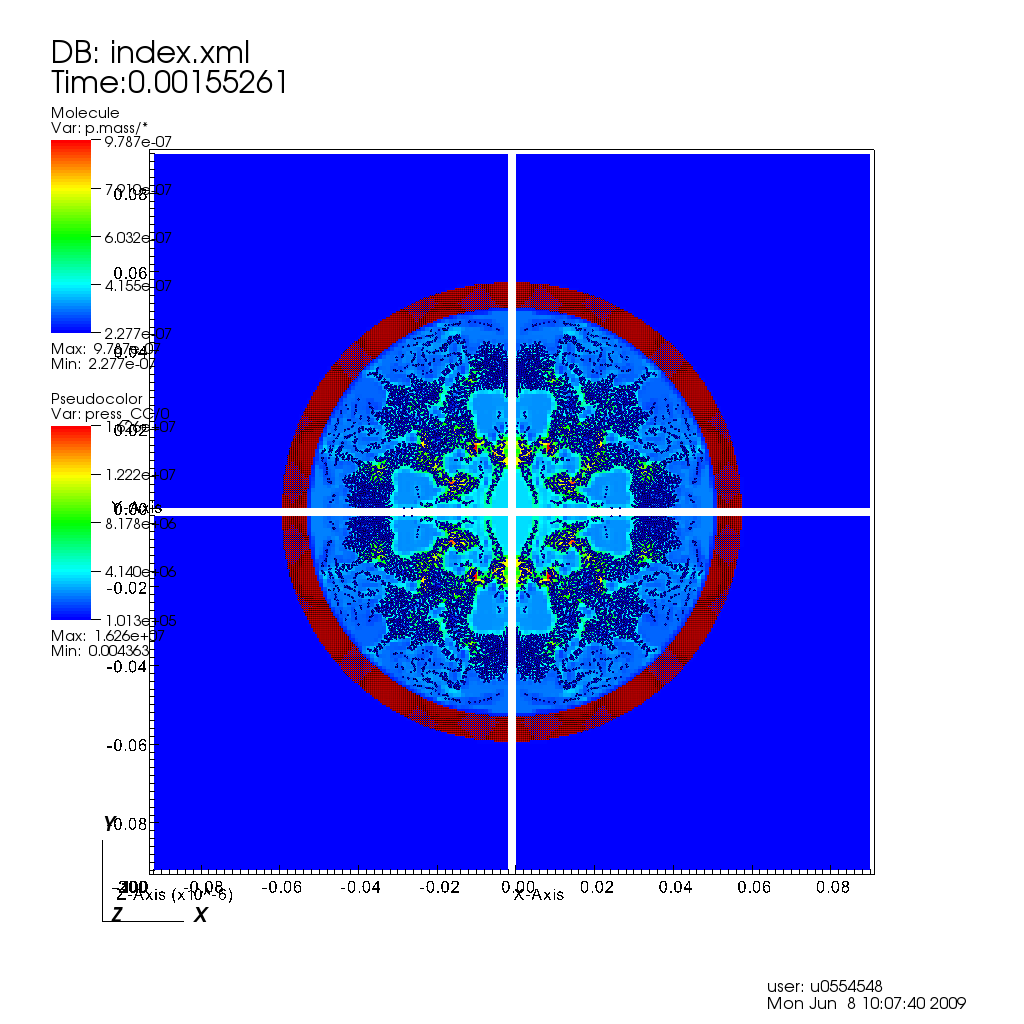
\includegraphics[scale=.3]{SteadyBurn0000.png}

  \caption{Collapse of PBX into hollow bore of explosive device.}
  \label{figsteadyburn1}
\end{figure}

\begin{figure}
  \center
  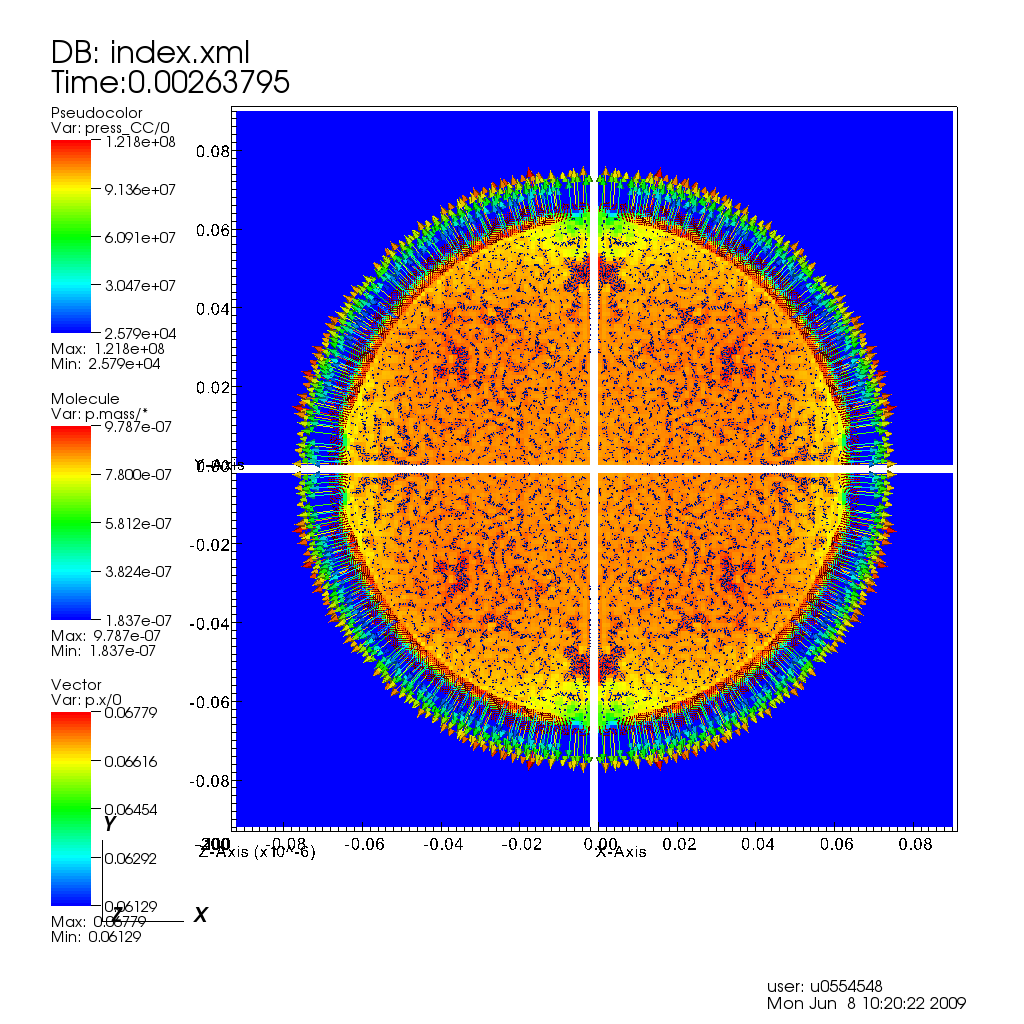
\includegraphics[scale=.4]{SteadyBurn0001.png}

  \caption{Expansion of steel casing as explosion occurs.}
  \label{figsteadyburn2}
\end{figure}

\begin{figure}
  \center
  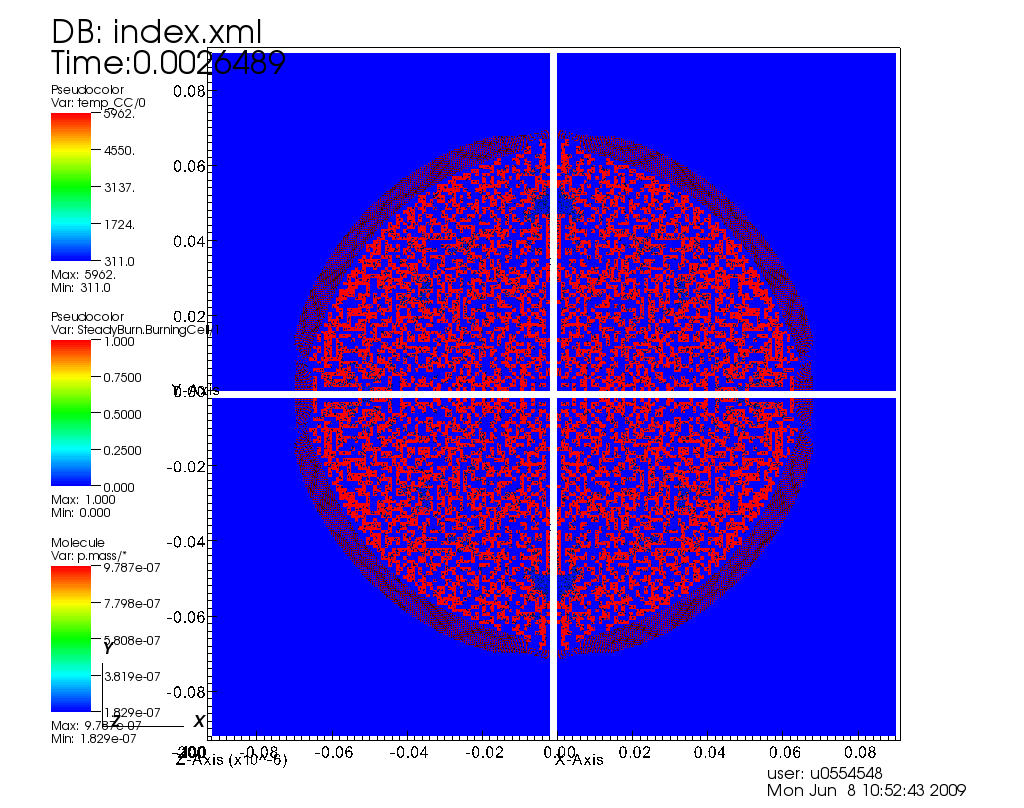
\includegraphics[scale=.4]{SteadyBurn0002.png}

  \caption{Burning Cells.}
  \label{figsteadyburn3}
\end{figure}

\newpage
%
\newpage
\section*{\center  T-Burner Example Using Unsteady Burn}
\addcontentsline{toc}{subsection}{T-Burner Example Using Unsteady Burn}
\subsection*{\underline{Problem Description}}
The T-Burner problem was inspired by  an article by Jerry Finlinson, Richard Stalnaker and Fred Blomshield in which a T-Burner apparatus was pressurized to a given pressure and ignited \cite{ref:finlinson1}.  The T-Burner composed of a cylinder with HMX on each circular ends, and a pressure inlet halfway between the HMX caps pumps pressure into the vessel parallel to those walls.  Finlinson, et. al. measured pressure oscillations in the chamber and this simulation mimics the behavior found of Finlinson's 500 psi experiment.  For simplicity and resource minimization, the simulation is set up as a 2D T-Burner.  The graphs below shows the pressure oscillations over time compared with that from \cite{ref:finlinson1}.  This simulation demonstrates the utility of Unsteady Burn in simulations where pressure oscillations occur in small places.  For more information on Unsteady Burn see \ref{Sec:UnsteadyBurn}.

\subsection*{\underline{Simulation Specifics}}
\begin{description}
\item [Component used:] \hfill mpmice (MPM-ICE)
\item [Input file name:] \hfill \TT{TBurner\_2dRT.ups}
\item [Command used to run input file:]\hfill mpirun -np 4 sus TBurner\_2dRT.ups

\item [Simulation Domain:]\hfill    0.822 x 0.138 x 0.003 m

\item [Example Runtimes:] \hfill \\
 25 minutes   (1 processor, 2.8 GHz Xeon)\\

\item [Physical time simulated:] \hfill 0.46 milliseconds \\ 
0.46 milliseconds of simulation equates flag $<$max\_Timesteps$>$410$</$max\_Timesteps$>$ \\ \\
Notes: \\
1)Remove line from input file to allow simulation to run full 0.25 seconds \\
2)Comment out $<$outputTimestepInterval$>$ and uncomment $<$outputInterval$>$ to make output $\Delta t$ constant \\ 

\item [Associated visit session:] \hfill TBurner.session

\end{description}

\newpage

\section*{\underline{Results}}

Figure~\ref{figtburn1}, ~\ref{figtburn2} and ~\ref{figtburn3} show successive snapshots of the simulation.  Contour plot depicts pressure and represents the wave front as it oscillates between two sheets of burning PBX 9501.  Figure ~\ref{figtburnVel} shows velocities of gas cells.
\begin{figure}
  \center
  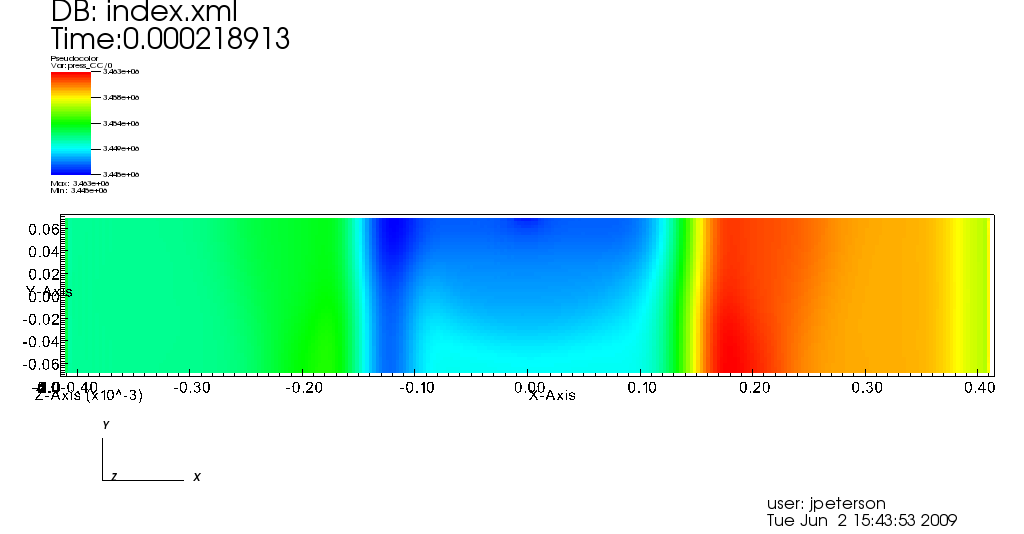
\includegraphics[scale=.4]{TBurner0000.png}

  \caption{Time 1: Oscillatory behavior in the form of a pressure wave in a T-Burner.  Contour plot depicts pressure.}
  \label{figtburn1}
\end{figure}

\begin{figure}
  \center
  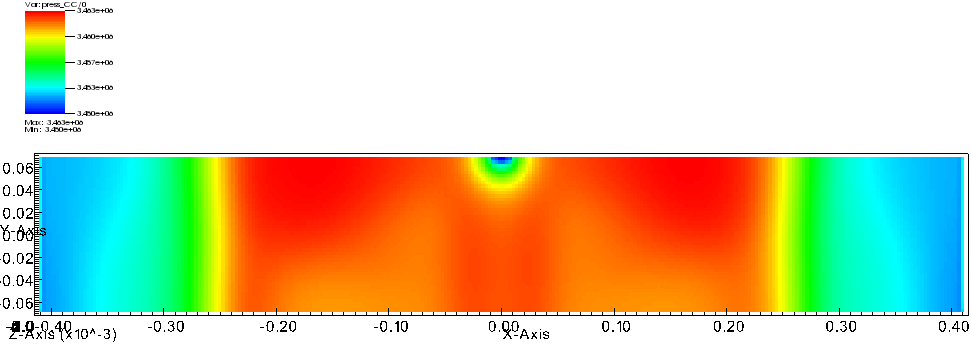
\includegraphics[scale=.4]{TBurner0001.png}

  \caption{Time 2: Oscillatory behavior in the form of a pressure wave in a T-Burner.  Contour plot depicts pressure.}
  \label{figtburn2}
\end{figure}
\begin{figure}
  \center
  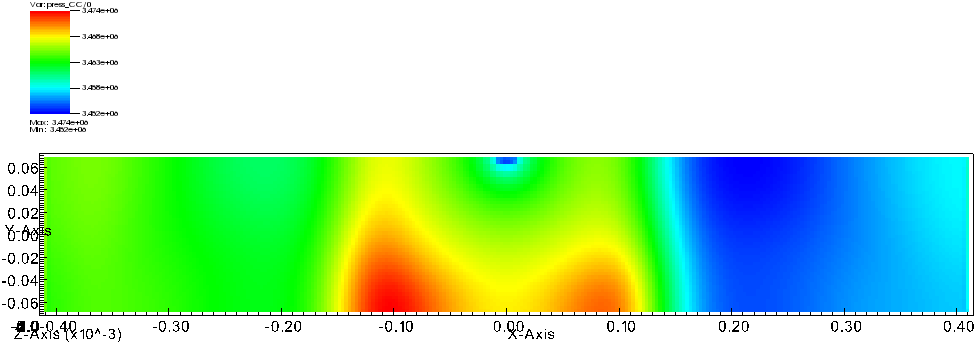
\includegraphics[scale=.4]{TBurner0002.png}

  \caption{Time 3: Oscillatory behavior in the form of a pressure wave in a T-Burner.  Contour plot depicts pressure.}
  \label{figtburn3}
\end{figure}

Figure~\ref{figtburnVel} shows a snapshot of the simulation at the same instant as the 
previous figure.  The contour plot depicts pressure.  The arrows are vectors depicting
the importance   
\begin{figure}
  \center
  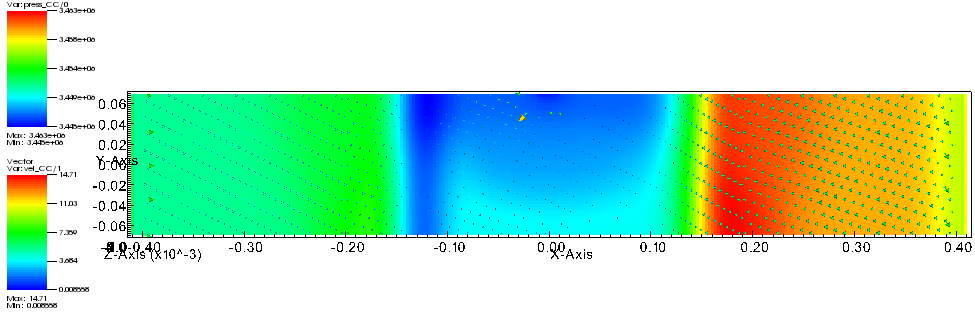
\includegraphics[scale=.4]{TBurnerVel0000.png}

  \caption{Velocity vectors of cell material.  Shows how the pressure causes gas to move.}
  \label{figtburnVel}
\end{figure}

%
%__________________________________
\subsection{References}
\bibliographystyle{plain}
\bibliography{ice}


\chapter{Wasatch}
The Wasatch documentation is available in a separate document located at "doc/Components/Wasatch".


\section{Glossary} \label{Sec:Glossary}

\begin{itemize}

\item Data Warehouse (NewDW, OldDW, DW) - The \tt Data Warehouse
         \normalfont is an abstraction (and implementation vehicle) used in
         Uintah to provide data to simulation components (across
         distributed memory spaces as necessary).  OldDW refers to a
         DW from the previous time step.  NewDW refers to the DW for
         the current time step.  In practice, variables are usually
         pulled from the OldDW, updated, and placed in the NewDW.

\item Time step - Uintah is a time dependent code.  A time step refers
         to a unique point in simulation time.  The state of the
         simulation is updated one time step at a time.
         
\item Adaptive Mesh Refinement (AMR) - In brief, AMR allows spending
  less CPU time on ``inactive'' (less interesting) areas of the
  simulation, and spend more time computing where there are many
  particles reacting.  Resolution is low in the center where things
  are stable, but high at the edges.  This feature is in ICE, but not
  ARCHES.

\item CCA - Common Component Architecture.

\item CFD - Computational Fluid Dynamics modeling.

\item DistCC - Parallel, distributed compiler.

\item Doxygen - Doxygen (code documentation) web interface.

\item GhostCells (and Extra Cells)

\item Grid - The problem's physical domain.  The number of cells in the
  grid determine the resolution of the simulation.

\item Handle - Smart pointers.  Handles track the number of references
  to a given object, and when the number reaches zero, de-allocates
  the memory.

\item Level - Not a 'level' in 3d-space, but a level of recursion into an
  AMR grid.  ARCHES doesn't support AMR or nonuniform cells, and
  therefore doesn't need recursion, so it works on a single level '1'.

\item Material Point Method (MPM) - The main component for simulating
  structures (physcial objects) in the UCF.

\item Message Passing Interface (MPI) - Communication library used by many
  distributed software packages to communicate data between multiple
  processors.  Besides send'ing and recv'ing data, data
  reduction (UCF Reduction Variables) is supported. 
  \begin{itemize}
    \item OpenMPI
  \end{itemize}

\item Patch - A physical region of the grid assigned one to each
  processor.  The processor working on a patch will compute properties
  for each of the cells contained in the patch.  Think of this as a big
  cube that contains hundreds of little cubes.

\item Regression Tester (RT) - Runs nightly accuracy, memory, and
  completion tests on Uintah simulations.

%\item <table border=''1'' cellpadding=''5'' width=''80%''><tr><td
%                                %bgcolor=''#eeeeff''><b>Programmers
%                                %Note:</b> Programming examples and
%                                %notes will appear like
%                                %this.</td></tr></table>

\item Uintah Software Organization
  \begin{itemize}
    \item Visualization
    \item scinew - a wrapper for the C++ new() function that allows for memory tracking.
  \end{itemize}

\item ssh - password-less hints.

\item SUS - Standalone Uintah Simulator.  This is the main executable
  program in the Uintah project.

\item SVN - Subversion code versioning system.

\item Uintah Computational Framework (UCF) - The core software
  infrastructure for Uintah.
  \begin{itemize}
    \item Variables
  \end{itemize}

\item Uintah - The general name of the C-SAFE simulation code.
  Sometimes also refered to as the UCF.  The name comes from the
  Uintah mountain range in Utah.

\item Uintah Problem Specification (UPS (Section~\ref{Sec:UPS})) - An XML based file used to
  specify Uintah simulation properties.


\end{itemize}


\end{document}
